\documentclass{llncs}


%% Some recommended packages.
\usepackage{booktabs}   %% For formal tables:
                        %% http://ctan.org/pkg/booktabs
%\usepackage{subcaption} %% For complex figures with subfigures/subcaptions
                        %% http://ctan.org/pkg/subcaption
\usepackage{latexsym}
%\usepackage{setspace}
\usepackage{cancel}
\usepackage{listings}
\usepackage{graphicx}
\usepackage{appendix}
\usepackage{amssymb}
\usepackage{stmaryrd}
\usepackage{amsmath}
\usepackage{leftidx}
\usepackage{mathtools}
\usepackage{paralist}
\usepackage{color}
\usepackage{mathrsfs}
\usepackage{tikz}
%\usepackage[draft]{minted}
\usepackage{amsthm}
\usetikzlibrary{shapes}
\usepackage[linesnumbered,ruled]{algorithm2e}

\pagestyle{plain}

%==========================================================
%!TEX root = popl2018.tex

\newcommand{\set}[1]{\{ #1 \}}
\newcommand{\sequence}[2]{(#1, \ldots, #2)}
\newcommand{\couple}[2]{(#1,#2)}
\newcommand{\pair}[2]{(#1,#2)}
\newcommand{\triple}[3]{(#1,#2,#3)}
\newcommand{\quadruple}[4]{(#1,#2,#3,#4)}
\newcommand{\tuple}[2]{(#1,\ldots,#2)}
\newcommand{\Nat}{\ensuremath{\mathbb{N}}}
\newcommand{\Rat}{\ensuremath{\mathbb{Q}}}
\newcommand{\Rea}{\ensuremath{\mathbb{R}}}
\newcommand{\Zed}{\ensuremath{\mathbb{Z}}}
%\newcommand{\true}{\top}
%\newcommand{\false}{\perp}
\newcommand{\bottom}{\perp}
%% \newcommand{\powerset}[1]{{\cal P}(#1)}
\newcommand{\npowerset}[2]{{\cal P}^{#1}(#2)}
\newcommand{\finitepowerset}[1]{{\cal P}_f(#1)}
\newcommand{\level}[2]{L_{#1}(#2)}
\newcommand{\card}[1]{\mbox{card}(#1)}
\newcommand{\range}[1]{\mathtt{ran}(#1)}
\newcommand{\astring}{s}

\newcommand{\Cc}{\mathcal{C}}


\newcommand {\notof}{\ensuremath{\neg}}
\newcommand {\myand}{\ensuremath{\wedge}}
\newcommand {\myor}{\ensuremath{\vee}}
\newcommand {\mynext}{\mbox{{\sf X}}}
\newcommand {\until}{\mbox{{\sf U}}}
\newcommand {\sometimes}{\mbox{{\sf F}}}
\newcommand {\previous}{\mynext^{-1}}
\newcommand {\since}{\mbox{{\sf S}}}
\newcommand {\fminusone}{\mbox{{\sf F}}^{-1}}
\newcommand {\everywhere}[1]{\mbox{{\sf Everywhere}}(#1)}



\newcommand{\aatomic}{{\rm A}}
\newcommand{\aset}{X}
\newcommand{\asetbis}{Y}
\newcommand{\asetter}{Z}

\newcommand{\avarprop}{p}
\newcommand{\avarpropbis}{q}
\newcommand{\avarpropter}{r}
\newcommand{\varprop}{{\rm PROP}} % Set of atomic propositions (for a given logic)

% formulae

\newcommand{\aformula}{\astateformula} % a formula
\newcommand{\aformulabis}{\astateformulabis} % another formula (when at least 2 are present)
\newcommand{\aformulater}{\astateformulater} % another formula (when at least 3 are present)
\newcommand{\asetformulae}{X}
\newcommand{\subf}[1]{sub(#1)}

\newcommand{\aautomaton}{{\mathbb A}}
\newcommand{\aautomatonbis}{{\mathbb B}}

\newcommand {\length}[1] {\ensuremath{|#1|}}



% Equivalences
\newcommand{\egdef}{\stackrel{\mbox{\begin{tiny}def\end{tiny}}}{=}} % =def=
\newcommand{\eqdef}{\stackrel{\mbox{\begin{tiny}def\end{tiny}}}{=}} % =def=
\newcommand{\equivdef}{\stackrel{\mbox{\begin{tiny}def\end{tiny}}}{\equivaut}} % <=def=>
\newcommand{\equivaut}{\;\Leftrightarrow\;}

\newcommand{\ainfword}{\sigma}

\newcommand{\amap}{\mathfrak{f}}
\newcommand{\amapbis}{\mathfrak{g}}

\newcommand{\step}[1]{\xrightarrow{\!\!#1\!\!}}
\newcommand{\backstep}[1]{\xleftarrow{\!\!#1\!\!}}

\newcommand {\aedge}[1] {\ensuremath{\stackrel{#1}{\longrightarrow}}}
\newcommand {\aedgeprime}[1] {\ensuremath{\stackrel{#1}{\longrightarrow'}}}
\newcommand {\afrac}[1] {\ensuremath{\mathit{frac}(#1)}}
\newcommand {\cl}[1] {\ensuremath{\mathit{cl}(#1)}}
\newcommand {\sfc}[1] {\ensuremath{\mathit{sfc}(#1)}}
\newcommand {\dunion} {\ensuremath{\uplus}}
\newcommand {\edge} {\ensuremath{\longrightarrow}}
\newcommand {\emptyword}{\ensuremath{\epsilon}}
\newcommand {\floor}[1] {\ensuremath{\lfloor #1 \rfloor}}
\newcommand {\intersection} {\ensuremath{\cap}}
\newcommand {\union} {\ensuremath{\cup}}
\newcommand {\vals}[2] {\ensuremath{\mathit{val}_{#2}(#1)}}



\newcommand {\pspace} {\textsc{pspace}}
\newcommand {\nlogspace} {\textsc{nlogspace}}
\newcommand {\logspace} {\textsc{logspace}}
\newcommand {\expspace} {\textsc{expspace}}
\newcommand {\np} {\textsc{np}}
\newcommand {\threeexptime} {\textsc{3exptime}}
\newcommand {\polytime} {\textsc{p}}
\newcommand{\twoexpspace}{\textsc{2expspace}}
\newcommand{\threeexpspace}{\textsc{3expspace}}
\newcommand {\nexptime} {\textsc{nexptime}}



\newcommand{\aalphabet}{\Sigma}     % an alphabet, A is already used for atoms
\newcommand{\aword}{\mathfrak{u}}
\newcommand{\awordbis}{\mathfrak{v}}



\newcommand{\aassertion}{P}
\newcommand{\aassertionbis}{Q}
\newcommand{\aexpression}{e}
\newcommand{\aexpressionbis}{f}
\newcommand{\avariable}{\mathtt{x}}
\newcommand{\uniquevar}{\mathtt{u}}
\newcommand{\uniquevarbis}{\mathtt{v}}
\newcommand{\avariablebis}{\mathtt{y}}
\newcommand{\avariableter}{\mathtt{z}}
\newcommand{\nullconstant}{\mathtt{null}}
\newcommand{\nilvalue}{nil}
\newcommand{\emptyconstant}{\mathtt{emp}}
\newcommand{\infheap}{\mathtt{inf}}
\newcommand{\saturated}{\mathtt{Saturated}}

\newcommand{\astateformula}{\phi}
\newcommand{\astateformulabis}{\psi}
\newcommand{\astateformulater}{\varphi}
%%
\newcommand{\separate}{\ast}
\newcommand{\sep}{\separate}
\newcommand{\size}{\mathtt{size}}
\newcommand{\sizeeq}[1]{\mathtt{size} \ = \ #1}
\newcommand{\alloc}[1]{\mathtt{alloc}(#1)}
\newcommand{\allocb}[2]{\mathtt{alloc}^{-1}[#2](#1)}
\newcommand{\isol}[1]{\mathtt{isoloc}(#1)}
\newcommand{\icell}{\mathtt{isocell}}
\newcommand{\malloc}{\mathtt{malloc}}
\newcommand{\cons}{\mathtt{cons}}
\newcommand{\new}{\mathtt{new}}
\newcommand{\free}[1]{\mathtt{free} \ #1}
\newcommand{\maxform}[1]{\mathtt{maxForms}(#1)}
\newcommand{\locations}[1]{\mathtt{loc}(#1)}
\newcommand{\values}{\mathtt{Val}}
\newcommand{\aheap}{\mathfrak{h}}
\newcommand{\avaluation}{\mathfrak{V}}
\newcommand{\heaps}{\mathcal{H}}
\newcommand{\astore}{\mathfrak{s}}
\newcommand{\stores}{\mathcal{S}}
\newcommand{\amodel}{\mathfrak{M}}
\newcommand{\alabel}{\ell}

\newcommand{\aprogram}{\mathtt{PROG}}
\newcommand{\programs}{\mathtt{P}}
\newcommand{\ctprograms}{\programs^{ct}}
\newcommand{\aninstruction}{\mathtt{instr}}
\newcommand{\ainstruction}{\mathtt{instr}}
\newcommand{\instructions}{\mathtt{I}}
\newcommand{\aguard}{\ensuremath{g}}
\newcommand{\guards}{\ensuremath{G}}
\newcommand{\domain}[1]{\mathtt{dom}(#1)}
\newcommand{\memory}{\stores\times\heaps}
\newcommand{\skipinstruction}{\mathtt{skip}}

\newcommand{\execution}{\mathtt{comp}}
\newcommand{\aux}{\mathtt{embd}}
\newcommand{\runof}{run}
\newcommand{\anexecution}{e}


\newcommand{\aletter}{\ensuremath{a}}
\newcommand{\aletterbis}{\ensuremath{b}}
\newcommand{\alocation}{\mathfrak{l}}

\newcommand{\pointsl}[1]{\stackrel{#1}{\hookrightarrow}}
\newcommand{\ppointsl}[1]{\stackrel{#1}{\mapsto}}
\newcommand{\ourhook}[1]{\stackrel{#1}{\hookrightarrow}}
\newcommand{\ltrue}{{\sf true}}
\newcommand{\lfalse}{{\sf false}}


\newcommand{\variables}{\mathtt{FVAR}}
\newcommand{\pvariables}{\mathtt{PVAR}}
\newcommand{\secvariables}{\mathtt{SVAR}}
\newcommand{\logique}[1]{\mathtt{FO}(#1)}



\newcommand{\atranslation}{\mathfrak{t}}
\newcommand{\nbpred}[1]{\widetilde{\sharp #1}}
\newcommand{\nbpredstar}[1]{\widetilde{\sharp #1}^{\star}}
\newcommand{\isolated}{\mathtt{isol}}
\newcommand{\stdmarks}{\mathtt{envir}}
\newcommand{\relation}[1]{\mathtt{relation}_{#1}}
\newcommand{\freevar}{\mathtt{FV}}
\newcommand{\notonmark}{\mathtt{notonenv}}
\newcommand{\InVal}[1]{\mathtt{InVal}\!\left(#1\right)}
\newcommand{\NotOnEnv}[1]{\mathtt{NotOnEnv}\!\left(#1\right)}
\newcommand{\PartOfVal}[1]{\mathtt{PartOfVal}\!\left(#1\right)}
%\newcommand{\nbpreds}[3]{\sharp #1 \geq #2}
\newcommand{\defstyle}[1]{{\emph{#1}}}

\newcommand{\cut}[1]{}
\newcommand{\interval}[2]{[#1,#2]}
\newcommand{\buniquevar}{\overline{\uniquevar}}
\newcommand{\bbuniquevar}{\overline{\overline{\uniquevar}}}
\newcommand{\magicwand}{\mathop{\mbox{$\mbox{$-~$}\!\!\!\!\ast$}}}
\newcommand{\wand}{\magicwand}
\newcommand{\septraction}{\stackrel{\hsize0pt \vbox to0pt{\vss\hbox to0pt{\hss\raisebox{-6pt}{\footnotesize$\lnot$}\hss}\vss}}{\magicwand}}
%% \newcommand{\reach}{\mathtt{reach}}
\mathchardef\mhyphen="2D % hyphen while in math mode

\newcommand{\adataword}{\mathfrak{dw}}
\newcommand{\adatum}{\mathfrak{d}}

\newcommand{\collectionknives}{\mathtt{ks}}
\newcommand{\collectionknivesfork}[1]{\mathtt{ksfs}_{=#1}}
\newcommand{\collectionknivesforks}{\mathtt{ksfs}}
\newcommand{\collectionkniveslargeforks}{\mathtt{kslfs}}


\newcommand{\acounter}{\mathtt{C}}

\newcommand{\fotwo}[3]{{\mbox{FO2}_{#1,#2}(#3)}}
\newcommand{\mtrans}[1]{t\!\left(#1\right)^{\Box}}
\newcommand{\mbtrans}[2]{\mtrans{#2}_{#1}}


\newcommand{\alogic}{\mathfrak{L}}


\newcommand{\semantics}[1]{\ensuremath{[ #1 ]}}


\newcommand{\adomino}{\mathfrak{d}}
\newcommand{\atile}{\mathfrak{d}}
\newcommand{\atiling}{\mathfrak{t}}

\newcommand{\hori}{\mathtt{h}}
\newcommand{\verti}{\mathtt{v}}
\newcommand{\domi}{\mathtt{d}}

\newcommand{\cpyrel}{\mathfrak{cp}}

\newcommand{\cntcmp}{\mathfrak{C}}

\newcommand{\heapdag}{\mathfrak{G}}

\newcommand{\onmainpath}{\mathtt{mp}}

\newcommand{\tree}{\mathtt{tree}}

%\newcommand{\tile}{\mathtt{tile}}

\newcommand{\type}{\mathtt{type}}

\newcommand{\ptype}{\mathtt{ptype}}

\newcommand{\exttype}{\mathtt{exttype}}

\newcommand{\anctypes}{\mathtt{AncTypes}}

\newcommand{\destypes}{\mathtt{DesTypes}}

\newcommand{\inctypes}{\mathtt{IncTypes}}

\newcommand{\treeic}{\mathtt{treeIC}}

\newcommand{\trs}{\mathfrak{trs}}


\newcommand{\nin}{\not \in}
\newcommand{\cupplus}{\uplus}
\newcommand{\aunarypred}{\mathtt{P}}


\newcommand{\hide}[1]{}

\newcommand{\eval}[2]{\llbracket#1\rrbracket_{#2}}
\newcommand\cur{\mathsf{cur}}
\newcommand\dom{\mathsf{dom}}
\newcommand\rng{\mathsf{rng}}

\newcommand\dd{\mathbb{D}}
\newcommand\nat{\mathbb{N}}


\newcommand\cA{\mathcal{A}}
\newcommand\cB{\mathcal{B}}
\newcommand\cC{\mathcal{C}}
\newcommand\cE{\mathcal{E}}
\newcommand\cG{\mathcal{G}}
\newcommand\Ll{\mathcal{L}}
\newcommand\cM{\mathcal{M}}
\newcommand\cP{\mathcal{P}}
\newcommand\cR{\mathcal{R}}
\newcommand\cS{\mathcal{S}}
\newcommand\cT{\mathcal{T}}

\newcommand\vard{\mathfrak{d}}

\newcommand\replaceall{\mathsf{replaceAll}}
\newcommand\indexof{\mathsf{IndexOf}}


\newcommand\strline{\mathsf{SL}}

\newcommand\pstrline{\mathsf{SL_{pure}}}

\newcommand\search{\mathsf{search}}

\newcommand\verify{\mathsf{verify}}

\newcommand\searchleft{\mathsf{searchLeft}}

\newcommand\searchlong{\mathsf{searchLong}}


\newcommand\pref{\mathsf{Pref}}

\newcommand\wprof{\mathsf{WP}}

\newcommand\vars{\mathsf{Vars}}

\newcommand\dep{\mathsf{Dep}}
\newcommand\ptn{\mathsf{Ptn}}

\newcommand\src{\mathsf{src}}
\newcommand\strtorep{\mathsf{strToRep}}

\newcommand\rpleft{\mathsf{l}}
\newcommand\rpright{\mathsf{r}}


\newcommand\srcnd{\mathsf{srcND}}

\newcommand\ctxt{\mathsf{ctxt}}


\newcommand\ctxts{\mathsf{Ctxts}}

\newcommand\sprt{\mathsf{sprt}}

\newcommand\val{\mathsf{val}}

\newcommand\srclen{\mathsf{srcLen}}

\newcommand\rpleftlen{\mathsf{lLen}}


\newcommand\dfs{\mathsf{DFS}}

\newcommand\repr{\mathsf{rep}}

\newcommand\red{\mathsf{red}}

\newcommand\gfun{\mathcal{F}}


\newcommand{\leftmost}{{\sf leftmost}}
\newcommand{\longest}{{\sf longest}}

\newcommand{\arbidx}{{\sf Idx_{arb}}}
\newcommand{\dmdidx}{{\sf Idx_{dmd}}}
\newcommand{\lftlen}{{\sf Len_{lft}}}

%\newtheorem{remark}[theorem]{Remark}

\newcommand{\OMIT}[1]{}
\newcommand{\defn}[1]{\emph{#1}}

\newcommand{\Left}{\ensuremath{-1}}
\newcommand{\Right}{\ensuremath{1}}
\newcommand{\Stay}{\ensuremath{0}}

\newcommand{\Aut}{\ensuremath{\mathcal{A}}}
\newcommand{\AutB}{\ensuremath{\mathcal{B}}}
\newcommand{\Transducer}{\ensuremath{T}}
\newcommand{\controls}{\ensuremath{Q}}
\newcommand{\finals}{\ensuremath{F}}
\newcommand{\transrel}{\ensuremath{\delta}}

\newcommand{\Lang}{\mathcal{L}}
\newcommand{\Tran}{\mathcal{T}}

\newcommand{\ialphabet}{\Sigma}
\newcommand{\oalphabet}{\Gamma}

\newcommand{\EndLeft}{\ensuremath{\vartriangleright}}
\newcommand{\EndRight}{\ensuremath{\vartriangleleft}}



%
% General
\newcommand\brac[1]{\left(#1\right)}
\newcommand\tup\brac


% Tiling

\newcommand\width{\ell}
\newcommand\height{h}
\newcommand\hcons{H}
\newcommand\vcons{V}
\newcommand\tiles{T}
\newcommand\tile{t}
\newcommand\inittile{t_0}
\newcommand\fintile{t_f}
\newcommand\rowdelim{\#}

% Reduction
\newcommand\resetchar{!}
\newcommand\bit{b}

% \nbit[i][0] = 0_i, similarly for 1
\newcommand\nbit[2]{#2_{#1}}

% \repl{n}{0}{1} = $^1_{n,0} means if nth bit is 0, turn into a 1
\newcommand\repl[3]{\$^{#3}_{#1, #2}}

%==========================================================

%\newcommand\shortlong[2]{#2}
\newcommand\shortlong[2]{#1}

\newif\ifdraft\drafttrue
%\newif\ifdraft\draftfalse
\ifdraft
\newcommand{\anthony}[1]{\color{red} {AL: #1 :LA} \color{black}}
\newcommand{\zhilin}[1]{\color{brown} {ZL: #1 :LZ} \color{black}}
\newcommand{\tl}[1]{\color{blue} {TL: #1 :LT} \color{black}}
\newcommand{\mat}[1]{\color{cyan} {MH: #1 :HM} \color{black}}
\else
\newcommand{\anthony}[1]{}
\newcommand{\zhilin}[1]{}
\newcommand{\tl}[1]{}
\newcommand{\mat}[1]{}
\fi

\newcommand{\concat} {\circ}
\newcommand{\replace} {{\sf replace}}
\newcommand{\str} {{\sf Str}}
\newcommand{\intnum} {{\sf Int}}
\newcommand{\regexp} {{\sf RegExp}}
\newcommand{\strarr} {{\sf StringArray}}
\newcommand{\dtypes} {{\sf DataTypes}}
\newcommand{\anarr} {{\mathbb{A}}}

%============================================================


\begin{document}

\title{Parametric Transducers}
\subtitle{(An Expressive Framework for Symbolic 
Execution Analysis of Programs with Strings)}

\author{}
\institute{}

\maketitle

%\zhilin{Parametric versus parameterised ?}

%!TEX root = popl2018.tex

\begin{abstract}

The theory of strings with concatenation has been widely argued as the basis of
constraint solving for verifying string-manipulating programs. However, this
theory is far from adequate for expressing many string constraints that are
also needed in practice; for example, the use of regular constraints (pattern matching
against a regular expression), and the string-replace function (replacing
either the first occurrence or all occurrences of a ``pattern'' string
constant/variable/regular expression by a ``replacement'' string
constant/variable), among many others. Both regular constraints and the
string-replace function are crucial for such applications as analysis of
JavaScript (or more generally HTML5 applications) against cross-site scripting
(XSS) vulnerabilities, which motivates us to consider a richer class of string
constraints. The importance of the string-replace function (especially the
replace-all facility) is increasingly recognised, which can be witnessed by the
incorporation of the function in the input languages of several string
constraint solvers. 

Recently, it was shown that any theory of strings containing the string-replace
function (even the most restricted version where pattern/replacement strings
are both constant strings) becomes undecidable if we do not impose some kind of
straight-line (aka acyclicity) restriction on the formulas. Despite this,
the straight-line restriction is still practically sensible since this condition is  
typically met by string constraints that are generated by symbolic   execution.
In this paper, we provide the first systematic study of straight-line string 
constraints with the string-replace function and the regular constraints as the 
basic operations. We show that a large class of such constraints (i.e. when
only a constant string or a regular expression is permitted in the
pattern) is decidable. We note that the string-replace function, even under
this restriction, is sufficiently powerful for expressing the concatenation
    operator and much more (e.g. extensions of regular expressions with string variables).
This gives us the most expressive decidable logic containing concatenation,
replace, and regular constraints under the same umbrella.
Our decision procedure for the straight-line fragment follows an 
    automata-theoretic approach, and is modular in the sense that the string-replace terms are removed one by one to generate more and more regular constraints, which can then be discharged by the state-of-the-art string constraint solvers. 
We also show that this fragment is, in a way, a maximal decidable subclass of
the straight-line fragment with the string-replace and regular constraints.
To this end, we show that undecidability results in the following two
extensions: (1) variables are permitted in the pattern parameter of
    the replace function, (2) length constraints are permitted.
    %, or character constraints, or constraints involving the IndexOf function are permitted in the logic.
    
    
    
    \OMIT{
    We also delineate the boundary of decidability by
    showing undecidability in the case of 
}
%In this paper, we revisit 
    %offer a different
%viewpoint of string constraints for 
\OMIT{
    the theoretical foundation of string constraints for verifying 
    string-manipulating programs and 
    offer a different viewpoint:  
    the string-replace function and regular constraints (i.e. 
    not concatenation) should be the basic operations. 

We first note that 
the most general version of the string-replace function (where the replacements are string
variables) 
is sufficiently powerful to express the concatenation operator, 
solving such constraints is undecidable in general. 
}
\OMIT{
We then impose a straight-line restriction on the formulas (a shape of
formulas typically generated by symbolic execution), and show that decidability
can be recovered for a large subclass of the resulting constraints, namely as
    long as the pattern string is not a variable (which is again undecidable). 


As a special subcase, we obtain the decidability of 

In addition, we show that adding either integer constraints, character constraints, or constraints involving the IndexOf function to the straight-line fragment leads to undecidability again.
}

%delineate
%the decidability boundary of the resulting fragments. Our main result is 
%an algorithm for deciding satisfiability for the straight-line fragment
%of formulas, wherein each pattern parameter is either a constant or a 
 %   a ``source'' variable (i.e. not defined in terms of other variables using
 %   the replace function). On one hand, our decidability result strictly 
 %   subsumes a recently proposed
%A large 
%decidable subclass of the theory of strings with concatenation, replace 
%(where both pattern/replacement strings must be constant strings), and 
%regular constraints, which could express the program logic of scripts with 
%subtle DOM-based XSS vulnerabilities. On the other hand, our decidability
%allows a natural usage of the replace function to be modelled (e.g., 
%replacing each occurrence of the string \texttt{'username'} by a username
%variable).
%particular,
    %by imposing the straight-line
%restriction on the formulas. This class of formulas 
%with equality of variables permitted solving such constraints is undecidable 
%in general. 
    %Concatenation can easily be
    %simulated by the most general version of string 
    %We observe that concatenation can
%be easily simulated by 
%The string-replace function in its most generality.  

    \OMIT{
Our goal in this paper is to investigate extensively the decidability and complexity of the satisfiability problem of string constraints with the function $\replaceall$. We show that while it is undecidable in general, the satisfiability problem for the straight-line fragment is in EXPSPACE, by following an automata-theoretical approach.
}
\end{abstract}


%!TEX root = popl2018.tex

\section{Introduction}

The problem of %satisfiability of logical theories over strings
automatically solving string constraints (aka satisfiability of logical theories over
strings) has recently witnessed
renewed interest %in the programming language and verification community
\cite{Berkeley-JavaScript,TCJ16,LB16,YABI14,S3,Abdulla14,Abdulla17,DV13,symbolic-transducer,BEK} 
because of important applications in the analysis of 
string-manipulating programs. For example,
program analysis techniques like symbolic execution \cite{king76,DART,EXE} 
would
%. For example, program analysis techniques like
%symbolic execution \cite{king76} (or variants like dynamic symbolic execution
%\cite{DART,EXE}) will 
systematically explore executions in a program and collect symbolic path 
constraints, which could then be solved using a constraint solver and
used to determine which location in the program to continue exploring.
To successfully apply a constraint solver in this instance, it is
crucial that the constraint language precisely model the data types in the
program, along with the data-type operations used. In the context of
string-manipulating programs, this could include 
concatenation, regular constraints (i.e. pattern matching against a regular
expression), string-length functions, and the string-replace functions, among 
many others.

%For scripting
%languages (e.g. Python, PHP, and JavaScript), which have grown in popularity
%in recent years, numerous string 
%There are several well-established research threads on this satisfiability 
%problem depending on 
%which string operations are permitted in the theory. 
Perhaps the most well-known theory of strings for applications to analysing
string-manipulating programs is the theory of strings with concatenation 
(aka \emph{word equations}),
whose decidability status was settled positively by Makanin \cite{Makanin}
in 1977 after it was open for many years. More importantly, 
this theory remains 
decidable even when regular constraints are incorporated into the 
language \cite{Schulz}. However, whether adding the string-length function
results preserves the decidability remains a long-standing open problem
\cite{Vijay-length,buchi}.

%\OMIT{
%which is crucial for 
Another important string operation (especially, in popular scripting
languages like Python, JavaScript, and PHP) is the string-replace function, 
which may be used to replace either the first occurrence or
all occurrences of a string (a string constant/variable, or a regular expression) by 
another string (a string constant/variable). The replace function (especially 
the replace-all functionality) is omnipresent in HTML5 applications
\cite{LB16,TCJ16,YABI14}. 
%\mat{What does it mean for the replace function to be convincingly argued?}
For example, a standard industry defense against cross-site scripting 
(XSS) vulnerabilities includes sanitising untrusted strings before adding them
into the DOM (Document Object Model) or the HTML document. 
This is typically done by %replacing every occurrence of
various metacharacter-escaping mechanisms (e.g. see 
\cite{Kern14,BEK,OWASP-XSS}), e.g., backslash-escape, which replaces \emph{every
occurrence} of quotes and double-quotes (i.e. \verb+'+ and \verb+"+) in the
string by \verb+\'+ and \verb+\"+. 
In addition
to sanitisers, common JavaScript functionalities like \texttt{document.write()} 
and \texttt{innerHTML} apply an \emph{implicit browser transduction} --- which
decodes HTML codes (e.g. \verb+&#39;+ is replaced by \verb+'+) in the input 
string --- before inserting the input string into the DOM.
Both of these examples can be expressed by (perhaps multiple) 
applications of the string-replace function.
Moreover, although these examples replace constants by constants, the popularity of template systems such as Mustache~\cite{Mustache} demonstrate the need for replacements involving variables.
Using Mustache, a web-developer, for example, may define an HTML fragment with placeholders that is instantiated with user data during the construction of the delivered page.
\mat{Need to say more what template systems are?}
\anthony{Better mention closure templates I think, Matt. They do both
mustache-kind of replace plus sanitisers. They call these strict autoescaping
templates. See \cite{SSS11}.}

%Concatenation: 8\%
%Replace-all: 8\%

In general, the string-replace function has three parameters, and in the current mainstream language such as Python and JavaScript, all of the three parameters can be inserted as string variables. As result, when we perform program analysis for, for instance, detecting security vulnerabilities as described as above, one often obtains string constraints of the form $z= \replaceall(x, p, y)$, where $x,y$ are string constants/variables, and $p$ is either a string constant/variable, or a regular expression.
Such a constraint means that $z$ is obtained by replacing all occurrences of $p$ in $x$ by $y$. For convenience, we call $x, p, y$ as the subject, the pattern, and the replacement parameters respectively. 

%for instance $z=\replaceall(x,"aa", y)$, meaning that $z$ is obtained by replacing all occurrences of $aa$ in $x$ by $y$. Solving string constraints involving this type of constraints is crucial, but unfortunately, is not supported by the current technique. There are two reasons:

%The string-replace function is formalised as $\replaceall(x, p, y)$, where $x,y$ are string constants/variables, and $p$ is either a string constant/variable, or a regular expression. The semantics of $\replaceall(x, p, y)$ is to replace all occurrences of $p$ in $x$ with $y$. For convenience, we call $x, p, y$ as the subject, the pattern, and the replacement parameters respectively. 

%The string-replace function is a quite powerful string operation. To see this, let us consider the constraint $C \equiv z = \replaceall(x, 0, y) \wedge x \in (01)^* \wedge y \in 0^*$. Then the set of values of $z$ that make $C$ satisfied is $\{(0^n 1)^* \mid n \in \Nat \}$.


The $\replaceall$ function is a powerful string operation that goes beyond the 
expressiveness of concatenation. 
Recently, it was shown in \cite{LB16} that any theory of strings containing the 
string-replace function (even the most restricted version where 
pattern/replacement strings are both constant strings) becomes undecidable if 
we do not impose some kind of
straight-line (aka acyclicity) restriction on the formulas. 
\OMIT{
As a matter of fact, it was shown in~\cite{LB16} that any 
incorporating a simple form of the $\replaceall$ function, where the pattern and the replacement are both string constants, into the theory of concatenations already results in an undecidable theory of strings.  
%that lies beyond 
%the expressiveness of the theory of concatenation, 
Therefore, it is challenging to reason about the string-replace function in its general form. 
}
%In~\cite{LB16}, a theory of strings involving concatenation and finite state transducers was considered. The $\replaceall$ function where the pattern is a string constant or regular expression, the third parameter is a constant can be seen as a special case of finite state transducers. It was shown therein that incorporating the simple form of the $\replaceall$ function into the theory of concatenations already results in an undecidable theory of strings. 
A partial result 
%can be deduced from the results 
from the following recent POPL paper in~\cite{LB16} provides decidability
for the straight-line fragment of the theory of strings involving 
concatenation, regular constraints, and the $\replaceall$ function where the 
pattern and the replacement are both string constants. 
The decision procedure therein was obtained for finite-state transducers, which
subsume the aforementioned simple form of the $\replaceall$ function, but
\emph{not} in its most form.
The straight-line restriction is natural in the sense that it reflects the shape of formulas typically generated by symbolic execution.  Nevertheless, the decidability boundary of the straight-line fragment of string constraints involving the $\replaceall$ function in this general form, e.g. when the replacement parameter is a variable, remains an open question which we address in this article.
\mat{Am i right to say we tackle it here?}

%% If you're looking for all the omitted and hidden semi-paragraphs that were here, checkout version 407adea8bf0c0564f064f43ae3b355fc8ac901d7. -- Matt

\paragraph{Example}

We give a simple example demonstrating a (naive) XSS vulnerability to illustrate the use of string-replace functions.
Consider the HTML fragment below.
\begin{minted}{html}
    <h1>User 
        <span onMouseOver="popupText('{{bio}}')">
            {{userName}} </span> </h1>
\end{minted}
This HTML fragment is a template as might be used with systems such as Mustache to display a user on a webpage.
For each user that is to be displayed -- with their username and biography stored in variables \emph{name} and \emph{biography} respectively -- the string \verb+{{userName}}+ will be replaced by \emph{name} and the string \verb+{{bio}}+ will be replaced by \emph{bio}.
For example, a user \verb+Amelia+ with biography \verb+Amelia was born in 1979...+ would result in the HTML below.
\begin{minted}{html}
    <h1>User 
        <span onMouseOver="popupText('Amelia was born in 1979...')">
            Amelia </span> </h1>
\end{minted}
This HTML would display \verb+User Amelia+, and, when the mouse is placed over \verb+Amelia+, her biography would appear, thanks to the \verb+onMouseOver+ attribute in the \verb+span+ element.

Unfortunately, this template could be insecure if the user biography is not adequately sanitised: 
A user could enter a malicious biography, such as \verb+'); alert('Boo!'); alert('+ which would cause the following instantiation of the \verb+span+ element\footnote{
    Readers familiar with Mustache may expect single quotes to be automatically escaped.
    However, this was not part of the specification until 2014, before which, support was inconsistent, which may have caught some developers off-guard~\cite{MustacheSingleQuote}.    
}.
\begin{minted}{html}
    <span onMouseOver="popupText(''); alert('Boo!'); alert('')">
\end{minted}
Now, when the mouse is placed over the user name, the malicious JavaScript \verb+alert('Boo!')+ is executed.

The presence of such malicious injections of code can be detected using string constraint solving and XSS \emph{attack patterns} $P$, which are given as regular expressions~\cite{BCFJKKV08,SAHMMS10,YABI14}.
For our example, given an attack pattern $P$ and template $t$, we would generate the constraint
\[
    x_1 = \replaceall(t, \verb+{{userName}}+, \mathit{user})
    \land
    x_2 = \replaceall(x_1, \verb+{{bio}}+, \mathit{bio})
    \land
    x_2 \in P
\]
which would detect if the HTML generated by instantiating the template is susceptible to the attack identified by $P$.
\mat{ANTHONY: can you verify/expand on my use of attack patterns?  I just copied it wholesale and blindly from your POPL 2016.}

\paragraph{Contribution.} We investigate the decidability boundary of the theory of strings involving concatenation, regular constraints, and the $\replaceall$ function, with the straight-line constraint introduced in \cite{LB16}. 

We first show that with the $\replaceall$ function in its general form, the concatenation operation is in fact \emph{redundant}, in the sense that it can be simulated by the $\replaceall$ function. This motivates us to consider a theory of strings where the $\replaceall$ function, instead of the concatenation operation, and the regular constraints, are the basic modalities. We focus on the straight-line fragment of this theory, denoted by $\strline[\replaceall]$.

We obtain the following results for the satisfiability problem of $\strline[\replaceall]$.
\begin{itemize}
\item If the pattern parameters of the $\replaceall$ function are allowed to be variables, then the satisfiability of $\strline[\replaceall]$ is undecidable (cf. Proposition~\ref{prop-und-pat-var}).
%
\item If the pattern parameters of the $\replaceall$ function are regular expressions, then the satisfiability of $\strline[\replaceall]$ is decidable and in EXPSPACE (cf. Theorem~\ref{thm-main}). In addition, we show that the satisfiability problem is PSPACE-complete for several cases that are meaningful in practice (cf. Corollary~\ref{cor-pspace}).
%
\item If $\strline[\replaceall]$, where the pattern parameters of the $\replaceall$ function are regular expressions, is extended with any of integer constraints, character constraints, or constraints involving the $\indexof$ function, then the satisfiability becomes undecidable again (cf. Theorem~\ref{thm-ext-int} and  Proposition~\ref{prop-ext-char}-\ref{prop-indexof}).
\end{itemize}

Our decision procedure for $\strline[\replaceall]$ where the pattern parameters of the $\replaceall$ function are regular expressions follows the automata-theoretical approach. The key idea is explained as follows: Let us consider the simple formula $C \equiv x = \replaceall(y, a, z) \wedge x \in e_1 \wedge y \in e_2 \wedge z \in e_3$. 
Suppose that $\cA_1,\cA_2,\cA_3$ are the nondeterministic finite state automata corresponding to $e_1,e_2,e_3$ respectively. 
We effectively eliminate the use of $\replaceall$ by nondeterministically generating from $\cA_1$ a new regular constraint $\cA'_2$ for $y$ -- and $\cA'_3$ for $z$ respectively -- that incorporates the effect of the $\replaceall$. Then the satisfiability of $C$ is turned into testing the nonemptiness of the intersection of $\cA_2$ and $\cA'_2$, as well as the nonemptiness of the intersection of $\cA_3$ and $\cA'_3$. When there are multiple occurrences of the $\replaceall$ function, this process can be iterated. 
Our decision procedure enjoys the following advantages:
\begin{itemize}
	\item it is automata-theoretic and built on a neat automata construction, moreover, when the formula is satisfiable, a solution can be synthesised, 
	
	\item the decision procedure is modular and amenable to implementation,  in the sense that the $\replaceall$ terms are removed one by one to generate more and more regular constraints,
	
	\item the decision procedure requires exponential space, but for the cases that are meaningful in practice, the decision procedure uses only polynomial space. 
\end{itemize}

%EXPSPACE algorithm
%
%a table to summarise the results.


\paragraph{Organisation.} 
This paper is organised as follows: Preliminaries are given in Section~\ref{sec-prel}. The core string language is defined in Section~\ref{sec-core}. The main results of this paper are summarised in Section~\ref{sec-sat}. The decision procedure is presented in Section~\ref{sec:replaceallsl}-\ref{sec:replaceallre}, case by case. The extensions of the core string language are investigated in Section~\ref{sec-ext}. The related work can be found in Section~\ref{sec-rel}.


%!TEX root = main.tex

\section{Preliminaries}
\label{sec:prelim}

\paragraph{General Notations.}
Let $\mathbb{Z}$ and $\Nat$ denote the set of integers and natural numbers
respectively. For $i \le j \in \Nat$, $[i, j]:=\{i,i+1,\ldots,j\}$ and
$[i] := [1, i]$. 
%\zhilin{The only place I notice that $[i] = [0,i]$ is used is the definition of semantics of \FFA{}(T). In most places, $[i]$ is used for $\{1,\ldots,i\}$. I would suggest to define $[i]=\{1,\ldots,i\}$, and if $[0,i]$ should be used, then just use $[0,i]$ there. I will assume this notation through the paper.} 
For a vector
$\vec{x}=(x_1,\cdots, x_n)$, let $|\vec{x}|$ denote the length of $\vec{x}$
(i.e., $n$) and  $\vec{x}[i]$ denote $x_i$ for each $i \in [n]$. For a set
$S$, we use $S^*$ (resp.~$S^+$) to denote the set of all finite (resp.~finite
and nonempty) sequences over $S$. We use $\epsilon$ for the empty sequence.
Given a function $f: A \to B$ and $X \subseteq B$, we use $f^{-1}(B)$ to
define the pre-image of $B$ under $f$, i.e., $\{ a \in A: f(a) \in B \}$.

%===================================================================================================
%=======================================================================
\OMIT{
\paragraph{Graph-Theoretical Notation.} \tl{not sure whether it is really needed; will see}
A DAG (\emph{directed acyclic graph}) $G$ is a finite directed graph $(V, E)$ with
no directed cycles, where $V$ (resp.~$E \subseteq V \times V$) is a set of vertices (resp.~edges).
%. That is, each DAG consists of finitely many vertices and edges, with each edge directed from one vertex to another, such that there is no way to start at any vertex $\mathit{v}$ and follow a consistently-directed sequence of edges that eventually loops back to $\mathit{v}$ again.
Equivalently, a DAG is a directed graph that has a topological ordering, which
is a sequence of the vertices such that every edge is directed from an earlier
vertex to a later vertex in the sequence. An edge $(\mathit{v},\mathit{v'})$ in
$G$ is called an \emph{incoming} edge of $\mathit{v'}$ and an \emph{outgoing}
edge of $\mathit{v}$. If $(\mathit{v},\mathit{v'}) \in E$, then $\mathit{v'}$ is
called a \emph{successor} of $\mathit{v}$ and $\mathit{v}$ is called a
\emph{predecessor} of $\mathit{v'}$. A \emph{path} $\pi$ in $G$ is a sequence
$\mathit{v}_0 \mathit{e}_1 \mathit{v}_1 \cdots \mathit{v}_{n-1} \mathit{e}_n
\mathit{v}_n$ such that for each $i \in [n]$, we have $\mathit{e}_i =
(\mathit{v}_{i-1},\mathit{v}_i) \in E$. The \emph{length} of the path $\pi$
%$\mathit{v}_0 e_1 \mathit{v}_1 \cdots \mathit{v}_{n-1} e_n \mathit{v}_n$ in $G$
is the number $n$ of edges in $\pi$. If there is a path from
$\mathit{v}$ to $\mathit{v'}$ (resp. from $\mathit{v'}$ to $\mathit{v}$) in $G$,
then $\mathit{v'}$ is said to be \emph{reachable} (resp. \emph{co-reachable})
from $\mathit{v}$ in $G$. If $\mathit{v}$ is reachable from $\mathit{v'}$ in
$G$, then $\mathit{v'}$ is also called an \emph{ancestor} of $\mathit{v}$ in
$G$. In addition, an edge $(\mathit{v'},\mathit{v''})$ is said to be reachable
(resp. co-reachable) from $\mathit{v}$ if $\mathit{v'}$ is reachable from $\mathit{v}$ (resp. $\mathit{v''}$ is co-reachable from $\mathit{v}$). The \emph{in-degree} (resp. \emph{out-degree}) of a vertex $\mathit{v}$ is the number of incoming (resp. outgoing) edges of $\mathit{v}$.
%A vertex $\mathit{v}$ in $G$ is said to be a \emph{join} vertex if the in-degree of $\mathit{v}$ is at least two.
%A DAG $G$ is called an \emph{arborescence} if there is a vertex $v_0$ such that all the vertices are reachable from $v_0$ in $G$, in addition, there are no join vertices in $G$.
A \emph{subgraph} $G'$ of $G=(V,E)$ is a directed graph $(V', E')$ with
$V' \subseteq V$ and $E' \subseteq E$. Let $G'$ be a subgraph of $G$. Then $G \setminus G'$ is the graph obtained from $G$ by removing all the edges in $G'$.
}
%=============================================================================
%=============================================================================================================


\paragraph{Automata.} We review some background from automata theory;
for more, see \cite{Kozen-automata,HU79}. Let $\ialphabet$ be a finite set (called
\defn{alphabet}). We usually define  $\overline{\ialphabet} := \ialphabet \cup \{\EndLeft,\EndRight\}$, where $\EndLeft,\EndRight\notin \Sigma$ are tape end markers for 2-way automata/transducer models. 
%\tl{I made  $\overline{\ialphabet}$ here as it used in multiple places}
 A sequence over $\ialphabet$ is called a \defn{string}. A \defn{language} is set of strings over $\ialphabet$.
We will review regular languages and necessary models of finite-state automata below.

\begin{definition}[Two-way finite-state automata] \label{def:2nfa}
    A \emph{(nondeterministic) two-way finite-state automaton}
(\FFA{}) over a finite alphabet $\ialphabet$ is a tuple $\Aut =
(\ialphabet, \EndLeft, \EndRight, \controls, q_0, \finals, \transrel)$ where 
    $\controls$ is a finite set of 
    states, $\EndLeft$ (resp.~$\EndRight$) a left (resp.~right) input tape end 
    marker, $q_0\in \controls$ is
the initial state, $\finals\subseteq \controls$ is a set of final states, and 
    $\transrel$ is the
transition relation  $\transrel\subseteq \controls \times 
    \overline{\ialphabet}\times \{\Left, \Stay, \Right\}\times \controls$. 
    %with $\overline{\ialphabet} := \ialphabet \cup \{\EndLeft,\EndRight\}$.
    Here, we assume %$\EndLeft, \EndRight \notin \ialphabet$, and 
    that
    there are no transitions that take the head of the tape past the left/right
    end marker (i.e.~$(p,\EndLeft,\Left,q), (p,\EndRight,\Right,q) \notin
    \transrel$ for every $p, q \in \controls$).
%\tl{not sure you want to use $\leftarrow, \rightarrow$?}
%    \anthony{Just defined macros. Please use generic macros in the definitions
%    guys.}

A (nondeterministic one-way) finite-state automaton (\FA{})
is a \FFA{} such that $\transrel \subseteq \controls \times \overline{\ialphabet} \times
    \{\Right,\Stay\} \times \controls $.
\end{definition}
Whenever understood we will only tacitly mention $\ialphabet$, 
$\EndLeft$, and $\EndRight$ in $\Aut$. 

%A \emph{nondeterministic finite automaton} (NFA) $\cA$ on $\Sigma$ is a tuple $(Q, \delta, q_0, F)$, where $Q$ is a finite set of \emph{states}, $q_0 \in Q$ is the \emph{initial} state, $F \subseteq Q$ is the set of \emph{final} states, and $\delta \subseteq Q \times \Sigma \times Q$ is the \emph{transition relation}.

The notion of runs of \FFA{} on an input string is exactly the same as that of
Turing machines on a read-only input tape. More precisely, for a string 
$w = a_1 \dots a_n$, a \emph{run} of $\Aut$ on $w$
%(with $a_0 = \EndLeft$ and $a_{n+1} = \EndRight$)
is a sequence of pairs $(q_0,i_0),\ldots, (q_m,i_m) \in \controls \times [0, n+1]$ 
defined as follows. Let $a_0 = \EndLeft$ and $a_{n+1} = \EndRight$. The
following conditions then have to be satisfied: $i_0 = 0$, and for every $j \in [m-1]$, we have $(q_j,a_{i_j}, dir, q_{j+1}) \in
	\transrel$ and $i_{j+1} = i_j + dir$ for some $dir \in  \{\Left, \Stay, \Right\}$.

%\begin{itemize}
%    \item $i_0 = 0$, and
%    \item for every $j \in [m-1]$, we have $(q_j,a_{i_j}, dir, q_{j+1}) \in
%        \transrel$ and $i_{j+1} = i_j + dir$ for some $dir \in  \{\Left, \Stay, \Right\}$.
%\end{itemize}
The run is said to be \defn{accepting} if $i_m = n+1$ and $q_m \in \finals$.
A string $w$ is \defn{accepted} by $\Aut$ if there is an accepting run of
$\Aut$ on $w$. The set of strings accepted by $\Aut$ is denoted by $\Lang(\Aut)$,
a.k.a., the language \defn{recognised} by $\Aut$.
%Since we deal with computational complexity in the sequel, we define
The \defn{size} $|\Aut|$ of $\Aut$ is defined to be $|\controls|$; this will
be needed when we talk about computational complexity.
%
For convenience, we will also refer to an \FA{} without initial and final states, that is, a pair $(Q, \delta)$, as a \emph{transition graph}.

%=======================================================================================

\OMIT{
state sequence $q_0 \dots q_n$ such that for each $i \in [n]$, $(q_{i-1}, a_i, q_i) \in \delta$. A run $q_0 \dots q_n$ is \emph{accepting} if $q_n \in F$. A string $w$ is \emph{accepted} by $\cA$ if there is an accepting run of $\cA$ on $w$. We use $\Ll(\cA)$ to denote the language defined by $\cA$, that is, the set of strings accepted by $\cA$. We will use $\cA, \cB, \cdots$ to denote NFAs.
%An NFA $\cA$ is \emph{deterministic} if for each $(q, \sigma) \in Q \times \Sigma$, there is at most one $q' \in Q$ such that $(q, a, q') \in \delta$. An NFA $\cA$ is \emph{complete} if for each $(q, \sigma) \in Q \times \Sigma$, there is at least one $q' \in Q$ such that $(q, a, q') \in \delta$. We assume that all NFA considered in this paper are complete.  An NFA $\cA$ is \emph{unambiguous} if for each string $w$, there is \emph{at most one accepting} run of $\cA$ on $w$.
For a string $w= a_1 \dots a_n$, we also use the notation $q_1 \xrightarrow[\cA]{w} q_{n+1}$ to denote the fact that there are $q_2,\dots, q_n \in Q$ such that for each $i \in [n]$, $(q_i, a_i, q_{i+1}) \in \delta$.  For an NFA $\cA=(Q, \delta, q_0, F)$ and $q, q' \in Q$, we use $\cA(q,q')$ to denote the NFA obtained from $\cA$ by changing the initial state to $q$ and the set of final states to $\{q'\}$. The \emph{size} of an NFA $\cA=(Q, \delta, q_0, F)$, denoted by $|\cA|$, is defined as $|Q|$, the number of states.

For convenience, we will also call an NFA without initial and final states, that is, a pair $(Q, \delta)$, as a \emph{transition graph}.
}
%============================================================================================

\FFA{} and \FA{} recognise precisely the same class of languages, i.e., 
\emph{regular languages}. The following result is standard and can be found in textbooks on automata theory
(e.g. \cite{Kozen-automata}). 

\begin{proposition}[\cite{HU79}]\label{prop-2nfa-nfa}
	Every \FFA{} $\Aut$ is equivalent to an \FA{} of size $2^{\bigO(|\Aut| \log |\Aut|)}$. 
%	Moreover, the equivalent
%    NFA can be computed in exponential time. 
    Moreover, every \FA{} can be transformed in polynomial time into an $\varepsilon$-free \FA{}, that is, an \FA{} where $\transrel\subseteq \controls \times \overline{\ialphabet} \times   \{\Right\} \times \controls $.
\end{proposition}
For latter reference, here we briefly mention the construction of \FA{}s from \FFA{}s in \cite{HU79}: For each  \FFA{} $\Aut=(\controls, q_0, \finals, \transrel)$, each state of the equivalent \FA{} is a vector of states from $\controls$ of \emph{odd} length, say $(q_1, \ldots, q_{2n+1})$, such that all the states of even (resp. odd) indices are mutually distinct.

In the rest of this paper, \FA{}s refer to $\varepsilon$-free \FA{}s where directions in transitions are omitted. Moreover, for simplicity of notations, in \FA{}s, we omit the two end markers $\EndLeft, \EndRight$ and assume that $\transrel \subseteq \controls \times \ialphabet \times    \{\Right,\Stay\} \times \controls$. 
%\zhilin{I assume that the two end markers are removed in FAs.}

\paragraph{Operations of \FA{}s.} For an FA $\Aut=(Q, q_0, F, \delta)$, $q \in Q$ and $P \subseteq Q$, we use $\Aut(q, P)$ to denote the FA $(Q, q, P, \delta)$, that is, the FA obtained from $\Aut$ by changing the initial state and the set of final states to $q$ and $P$ respectively. We use $q \xrightarrow[\Aut]{w} q'$ to denote the fact that a string $w$ is accepted by $\Aut(q, \{q'\})$. 


Given two \FA{}s $\Aut_1 = (Q_1, q_{0,1}, F_{1}, \delta_1)$ and $\Aut_2 = (Q_2, q_{0,2}, F_2, \delta_2)$, the \emph{product} of $\Aut_1$ and $\Aut_2$, denoted by $\Aut_1 \times \Aut_2$, is defined as $(Q_1 \times Q_2, (q_{0,1}, q_{0,2}), F_1 \times F_2, \delta_1 \times \delta_2)$, where $\delta_1 \times \delta_2$ is the set of tuples $((q_1,q_2), a, (q'_1, q'_2))$ such that $(q_1, a, q'_1) \in \delta_1$ and $(q_2, a, q'_2) \in \delta_2$. Evidently, we have $\Lang(\Aut_1 \times \Aut_2) = \Lang(\Aut_1) \cap \Lang(\Aut_2)$.


%%
%
%
%\anthony{I've removed the ``regular languages'' paragraph because it seems
%unnecessary. I recommend that operation on sets can be defined in General
%Notation above on general sets.}
%%\tl{Other relevant models such as SST, when appropriate, will be put here.}
%
%\zhilin{Let us fix the abbreviations here: \\
%--\FFA{}(2FT): two-way finite-state automata(transducer),\\
%--FA(FT): finite-state automata(transducer),\\
%--2PT: two-way parametric transducer,\\
%--PT: parametric transducer,\\
%--2SA(2ST): two-way symbolic automata(transducer),\\
%--SA(ST): symbolic automata(transducer) \\
%--2SPT: two-way symbolic parametric transducer,\\
%--SPT: symbolic parametric transducer 
%}
%\anthony{Can you please introduce macros?}


%%========= computational complexity==========================

\paragraph{Computational complexity:} In this paper, we study decision procedures and complexity of path feasibility problem of programs with strings. 
Pinpointing the precise complexity of verification problems is not only of fundamental
importance, but also it often suggests algorithmic techniques
that are most suitable for attacking the problem in practice.
We will deal with the following computational complexity
classes (see \cite{1994-papadimitriou} for more details): $\expspace$ (problems solvable
in exponential space), $n$-$\expspace$ (problems solvable in $n$-fold exponential space), nonelementary (problems that cannot be solved in $n$-fold exponential
time or space for every fixed $n > 0$).


 
%===================================================================
 
\OMIT{
\paragraph{Regular Languages.}
Fix a finite \emph{alphabet} $\Sigma$. Elements in $\Sigma^*$ are called \emph{strings}. Let $\varepsilon$ denote the empty string and  $\Sigma^+ = \Sigma^* \setminus \{\varepsilon\}$. We will use $a,b,\cdots$ to denote letters from $\Sigma$ and $u, v, w, \cdots$ to denote strings from $\Sigma^*$. For a string $u \in \Sigma^*$, let $|u|$ denote the \emph{length} of $u$ (in particular, $|\varepsilon|=0$). A \emph{position} of a nonempty string $u$ of length $n$ is a number $i \in [n]$ (Note that the first position is $1$, instead of  0). In addition, for $i \in [|u|]$, let $u[i]$ denote the $i$-th letter of $u$.
For two strings $u_1, u_2$, we use $u_1 \cdot u_2$ to denote the \emph{concatenation} of $u_1$ and $u_2$, that is, the string $v$ such that $|v|= |u_1| + |u_2|$ and for each $i \in [|u_1|]$, $v[i]= u_1[i]$ and for each $i \in |u_2|$, $v[|u_1|+i]=u_2[i]$. Let $u, v$ be two strings. If $v = u \cdot v'$ for some string $v'$, then $u$ is said to be a \emph{prefix} of $v$. In addition, if $u \neq v$, then $u$ is said to be a \emph{strict} prefix of $v$. If $u$ is a prefix of $v$, that is, $v = u \cdot v'$ for some string $v'$, then
we use $u^{-1} v$ to denote $v'$. In particular, $\varepsilon^{-1} v = v$.

A \emph{language} over $\Sigma$ is a subset of $\Sigma^*$. We will use $L_1, L_2, \dots$ to denote languages. For two languages $L_1, L_2$, we use $L_1 \cup L_2$ to denote the union of $L_1$ and $L_2$, and $L_1 \cdot L_2$ to denote the concatenation of $L_1$ and $L_2$, that is, the language $\{u_1 \cdot u_2 \mid u_1 \in L_1, u_2 \in L_2\}$. For a language $L$ and $n \in \Nat$, we define $L^n$, the \emph{iteration} of $L$ for $n$ times, inductively as follows: $L^0=\{\varepsilon\}$ and $L^{n} =L \cdot L^{n-1}$ for $n > 0$. We also use $L^*$ to denote the iteration of $L$ for arbitrarily many times, that is, $L^* = \bigcup \limits_{n \in \Nat} L^n$. Moreover, let $L^+ = \bigcup \limits_{n \in \Nat \setminus \{0\}} L^n$.

\begin{definition}[Regular expressions $\regexp$]
	\[e \eqdef \emptyset \mid \varepsilon \mid a \mid e + e \mid e \concat e \mid e^*, \mbox{ where } a \in \Sigma. \]
	Since $+$ is associative and commutative, we also write $(e_1 + e_2) + e_3$ as $e_1 + e_2 + e_3$ for brevity. We use the abbreviation $e^+ \equiv e \concat e^*$. Moreover, for $\Gamma = \{a_1, \cdots, a_n\}\subseteq \Sigma$, we use the abbreviations $\Gamma \equiv a_1 + \cdots + a_n$ and $\Gamma^\ast \equiv (a_1 + \cdots + a_n)^\ast$.
\end{definition}
We define $\Ll(e)$ to be the language defined by $e$, that is, the set of strings that match $e$, inductively as follows: $\Ll(\emptyset) =\emptyset$,
%\begin{itemize}
%\item
$\Ll(\varepsilon) =\{\varepsilon\}$,
%
%\item
$\Ll(a)= \{a\}$,
%
%\item
$\Ll(e_1 + e_2) = \Ll(e_1) \cup \Ll(e_2)$,
%
%\item
$\Ll(e_1 \concat e_2) = \Ll(e_1) \cdot \Ll(e_2)$,
%
%\item
$\Ll(e_1^*)=(\Ll(e_1))^*$.
%\end{itemize}
In addition, we use $|e|$ to denote the number of symbols occurring in $e$.

%A \emph{nondeterministic finite automaton} (NFA) $\cA$ on $\Sigma$ is a tuple $(Q, \delta, q_0, F)$, where $Q$ is a finite set of \emph{states}, $q_0 \in Q$ is the \emph{initial} state, $F \subseteq Q$ is the set of \emph{final} states, and $\delta \subseteq Q \times \Sigma \times Q$ is the \emph{transition relation}. For a string $w = a_1 \dots a_n$, a \emph{run} of $\cA$ on $w$ is a state sequence $q_0 \dots q_n$ such that for each $i \in [n]$, $(q_{i-1}, a_i, q_i) \in \delta$. A run $q_0 \dots q_n$ is \emph{accepting} if $q_n \in F$. A string $w$ is \emph{accepted} by $\cA$ if there is an accepting run of $\cA$ on $w$. We use $\Ll(\cA)$ to denote the language defined by $\cA$, that is, the set of strings accepted by $\cA$. We will use $\cA, \cB, \cdots$ to denote NFAs.
%%An NFA $\cA$ is \emph{deterministic} if for each $(q, \sigma) \in Q \times \Sigma$, there is at most one $q' \in Q$ such that $(q, a, q') \in \delta$. An NFA $\cA$ is \emph{complete} if for each $(q, \sigma) \in Q \times \Sigma$, there is at least one $q' \in Q$ such that $(q, a, q') \in \delta$. We assume that all NFA considered in this paper are complete.  An NFA $\cA$ is \emph{unambiguous} if for each string $w$, there is \emph{at most one accepting} run of $\cA$ on $w$.
%For a string $w= a_1 \dots a_n$, we also use the notation $q_1 \xrightarrow[\cA]{w} q_{n+1}$ to denote the fact that there are $q_2,\dots, q_n \in Q$ such that for each $i \in [n]$, $(q_i, a_i, q_{i+1}) \in \delta$.  For an NFA $\cA=(Q, \delta, q_0, F)$ and $q, q' \in Q$, we use $\cA(q,q')$ to denote the NFA obtained from $\cA$ by changing the initial state to $q$ and the set of final states to $\{q'\}$. The \emph{size} of an NFA $\cA=(Q, \delta, q_0, F)$, denoted by $|\cA|$, is defined as $|Q|$, the number of states. For convenience, we will also call an NFA without initial and final states, that is, a pair $(Q, \delta)$, as a \emph{transition graph}.

It is well-known (e.g. see \cite{HU79}) that regular expressions and \FA{}s are
expressively equivalent, and generate precisely all \emph{regular languages}.
In particular, from a regular expression, an equivalent \FA{} can be constructed
in linear time. Moreover, regular languages are closed under Boolean
operations, i.e., union, intersection, and complementation.
In particular, given two \FA{} $\cA_1=(Q_1, \delta_1, q_{0,1}, F_1)$ and
$\cA_2=(Q_2, \delta_2, q_{0,2}, F_2)$ on $\Sigma$, the intersection $\Ll(\cA_1)
\cap \Ll(\cA_2)$ is recognised by the \emph{product automaton} $\cA_1 \times
\cA_2$ of $\cA_1$ and $\cA_2$ defined as $(Q_1 \times Q_2, \delta, (q_{0,1}, q_{0,2}), F_1 \times F_2)$, where $\delta$ comprises the transitions $((q_1, q_2), a, (q'_1, q'_2))$ such that $(q_1, a, q'_1) \in \delta_1$ and $(q_2, a, q'_2) \in \delta_2$.
}
%==========================================================================================


%!TEX root = main.tex

\section{The Framework: Transducers, Straight-Line Programs}
\label{sec:framework}

In this section we first review the framework of straight-line programs from
\cite{LB16} for analysing symbolic execution of programs with strings, which
involves capturing ``built-in'' functions using finite-state transductions.
We will then introduce the notion of parametric transducers, and show that
they can capture many other interesting string functions that cannot be captured
within the framework of \cite{LB16}. In particular, this allows us to capture
string functions $f: (\Sigma^*)^k \to \Sigma^*$ with multiple input strings
(e.g. the replaceall function), and the string reverse function. 
The framework of straight-line programs from \cite{LB16} can be adapted
to this new notion of transducers, whose path feasibility problem, defined below, will be shown
to be decidable in Section \ref{sec:algo}.


%\anthony{Some abbreviations: 
%\begin{itemize}
%    \item 2PT, two-way parametric transducers
%    \item 1PT, one-way parametric transducers
%    \item 2RPT, two-way reversal-bounded parametric transducers
%    \item 2T, two-way non-parametric transducers
%    \item 1T, one-way non-parametric transducers
%\end{itemize}
%}

\subsection{A symbolic execution analysis framework} \label{subsec:symexe} 
As elegantly described in Bj\"{o}rner \emph{et al.} \cite{BTV09}, constraints 
from symbolic 
execution on string-manipulating programs can be viewed as the problem of \emph{path 
feasibility} over \emph{loopless} string-manipulating programs $S$ with variable
assignments and assertions, i.e., generated by the grammar
\begin{equation*}
    S ::= \qquad y := f(x_1,\ldots,x_n) \ |\ \text{\ASSERT{$g(x_1,\ldots,x_n)$}}\ |\ 
            S_1; S_2\ 
    %a ::= f(x_1,\ldots,x_n), \qquad b ::= g(x_1,\ldots,x_n) 
\end{equation*}
where $f: (\Sigma^*)^n \to \Sigma^*$ and $g: (\Sigma^*)^n \to \{0,1\}$ are
some string functions. That is, each symbolic execution $S$ is simply a program 
without loop or branching. 
The syntaxes for the functions $f$ and $g$ are now
left undefined, but will be instantiated as one explores algorithmic issues.
%with additional assertions on the way. 
%\mat{Should the ``straight-line'' restriction be explicitly defined?}
The problem of \defn{path feasibility}
asks whether, for a given program $S$, there exist \emph{input} strings (i.e. 
instantiations of variables that do not appear on left-hand side of an 
assignment) that take
$S$ to the end of the program while satisfying all the assertions. 
In general, it is useful to allow $f$ to be %\emph{partial} functions or, more
%generally, 
binary relations viewed as functions (as in programming, not mathematics) that 
nondeterministically choose an output string corresponding to an input string. 
For example, the 
notation $x := ?$ is common in the program verification to 
denote a nondeterministic assignment to $x$. More generally, nondeterministic
behaviour could be needed due to unknown inputs from a human user or other 
sources (e.g. databases). In this case, path feasibility of a
symbolic execution $S$
is defined in an \emph{angelic} way: each function in $S$
should be to produce \emph{some} output strings that take $S$ to the end of the
program.
%while satisfying all the assertions.
%Straight-line programs with assertions 

Symbolic executions can be viewed as constraints over the 
string domain by turning them
into a \emph{Static Single Assignment} (SSA) form (i.e. introduce a new 
variable 
on the left hand side of each assignment). See Figure \ref{fig:SSA} for an
example.
\begin{figure}
    \qquad
    \begin{minipage}{.49\linewidth}
        $x := x + \text{\texttt{aba}} + y$;\\
        $y := \text{replaceAll}(x,\texttt{a},\texttt{c})$;\\
        \ASSERT{$y \in \texttt{b}^*$}
    \end{minipage}
    \quad
    \begin{minipage}{.49\linewidth}
        $x_1 = x + \texttt{aba} + y\ \wedge$ \\
        $y_1 = \text{replaceAll}(x_1,\texttt{a},\texttt{c})\ \wedge$ \\
        $y_1 \in \texttt{b}^*$
    \end{minipage}
    \caption{String constraint (right) corresponding to a symbolic execution
    (left)
    \label{fig:SSA}}
\end{figure}

\emph{To avoid notational clutter, in the sequel we will follow \cite{BTV09}
and treat string 
constraints simply as symbolic executions in SSA form}, i.e., instead of 
conjunctions of atomic formulas from some logical theories. 
This simplifies 
the presentation of our decidable string logics and others in the literature 
(e.g. \cite{LB16,CCHLW18}) without obfuscating the connection to logic.


\subsection{The ``straight-line'' framework}
Bj\"{o}rner \emph{et al.} \cite{BTV09} initiated the exploration
of what kind of string functions $f$ and $g$ for which the above path 
feasibility problem can be algorithmically solved. 
One clean and powerful way to achieve decidability is to 
%functions $f$ and $g$
%in the assignments/conditionals is to 
allow some form of finite-state transducers in the definitions of $f$
and $g$.
%question of incorporating some form of transducers into the definitions of 
%
%the string functions $f$ and $g$ were briefly explored in \cite{BTV09}. 
This proposal was already explored in \cite{BTV09}, wherein the authors mention
that
%
%In
%summary, whenever all 
if the string functions $f$ and $g$ in the program can be captured by 
synchronised $k$-track finite automata (a.k.a.~\defn{automatic structures} 
\cite{BG04}), then
the path feasibility problem becomes decidable. They noted, however, that
this is too narrow for applications since string concatenation cannot be
captured in this framework. 

In a recent paper \cite{LB16}, Lin and Barcelo 
proposed allowing concatenation, regular constraints (i.e. regular expression 
matching), and \emph{one-way} finite-state transducers (not synchronised as in \cite{BTV09}, but only permits one input string and one output string) in 
straight-line programs. Finite transducers are a classic concept from
the theory of formal languages (e.g. see \cite{Berstel}).
%We will define finite-state
%transducers in the following subsection, but 
Roughly speaking, a finite transducer is an NFA with an extra output (write-only) 
track, i.e., upon reading an input symbol, it may decide to output (or not output) a symbol 
on the output track. We will define this in more detail below.
In general, the input/output tracks of finite-state transducers may be 
\emph{asynchronous}, which means that they cannot be captured by automatic structures of \cite{BG04}. 
Finite-state transducers are powerful for modelling many
different string functions including sanitisation functions (e.g. htmlescape and
backslash-escape) and implicit browser transductions in HTML5 applications (e.g.
innerHTML). Although they noted that this is
undecidable by the result of \cite{BFL13}, decidability can be obtained 
by disallowing \emph{string equality checks in the assertions $g$}, i.e., after
a simplification, we may assume that $g$ contains only regular constraints.
%In
%particular, an application of finite-state transducer and string equality checks
%are prohibited in $g$. 
The 
resulting class of string constraints is dubbed \emph{the straight-line 
fragment}.
They showed that the straight-line fragment is sufficiently powerful in
interesting applications including analysis of cross-site scripting (XSS)
vulnerabilities. 
%as we do not have these extensions, comment the following sentences out. 
%Decidable extensions of the straight-line fragment (including
%length constraints and disequality checks) were given by the authors, which 
%we will discuss in Section \ref{sec:extensions}.

The following is the precise definition
of two-way and one-way finite-state transducers.
\begin{definition}[Finite-State Transducers]
    Let $\ialphabet$ an alphabet.
    A \emph{nondeterministic two-way (finite) \emph{transducer}} (2NFT) over 
    $\ialphabet$ is a tuple $\Transducer = (\ialphabet, \EndLeft, \EndRight, \controls, q_0, \finals, \transrel)$ where  $\controls$, $\EndLeft$, $\EndRight$, $q_0$ are precisely the same as those of Definition~\ref{def:2nfa}
%    $\controls$ is a finite set of 
%    states, $\EndLeft$ (resp.~$\EndRight$) a left (resp.~right) input tape end 
%    marker, $q_0\in \controls$ is
%the initial state, $\finals\subseteq \controls$ is a set of final states, 
%
and 
    $\transrel$ is the
transition relation  $\transrel\subseteq \controls \times 
    \overline{\ialphabet}\times \{\Left, \Stay, \Right\}\times 
    \controls \times \ialphabet$ with
    $\overline{\ialphabet} := \ialphabet \cup \{\EndLeft,\EndRight\}$.
    Here, we assume $\EndLeft, \EndRight \notin \ialphabet$, and that
    there are no transitions that take the head of the tape past the left/right
    end marker. 

    A (nondeterministic one-way finite) transducer (NFT) over
    $\ialphabet$
    is a 2NFT whose transition relation contains only tuples of the form
    $(p,a,dir,q,b)$, where $dir \in \{\Stay,\Right\}$.
\end{definition}

%\anthony{Define the semantics of 2NFT as function $f: \ialphabet^* \to
%\ialphabet^*$}.\zhilin{Semantics defined below. Please check.}


The notion of runs of 2NFTs on an input string can be seen as a generalisation 
of 2NFA by adding outputs. More precisely, given a string $w = a_1 \dots a_n$, a \emph{run} of $\Transducer$ on $w$
%(with $a_0 = \EndLeft$ and $a_{n+1} = \EndRight$)
is a
sequence of tuples $(q_0, i_0, b_0),\ldots, (q_m, i_m, b_m) \in \controls \times (\{0\} \cup [n+1]) \times \Sigma$ 
such that, let $a_0 =\ \EndLeft$ and $a_{n+1} =\ \EndRight$, %. The following conditions, then, have to be satisfied:
\begin{itemize}
    \item $i_0 = 0$, and
    \item for every $j \in [m-1]$, $(q_j, a_{i_j}, dir, q_{j+1}, b_j) \in
        \transrel$, and $i_{j+1} = i_j + dir$ for some $dir \in \{\Left, \Stay, \Right\}$.
\end{itemize}
The run is said to be \defn{accepting} if $i_m = n+1$ and $q_m \in \finals$. When a run is accepting, $b_0 \cdots b_m$ is said to be the \emph{output} of the run.
A word $w'$ is said to be an output of $\Transducer$ on $w$ if there is an accepting run of
$\Transducer$ on $w$ with output $w'$. We use $\Tran(\Transducer)$ to denote the \emph{transduction} defined by $\Transducer$, that is, the relation comprising the pairs $(w,w')$ such that $w'$ is an output of $\Transducer$ on $w$.

%\tl{I propose we unify the term: e.g., using string instead of word}
%\anthony{I think it doesn't matter too much if we use both word/string. My
%suggestion is to try to use one \emph{more often}}

%============ removed, as agreed that rb will not be included. =========================
%\paragraph{Reversal-bounded transducers.}    
%Let $(q_0, i_0, b_0),\ldots, (q_m, i_m, b_m) $ be a run of $\Transducer$ on some string $w$. A \emph{reversal} of the run is a maximal subsequence $(q_j, i_j , b_j), \cdots, (q_{j'}, i_{j'}, b_{j'})$ where the direction of the reading head is reversed. More precisely, it is a maximal subsequence $(q_j, i_j , b_j), \cdots, (q_{j'}, i_{j'}, b_{j'})$ satisfying one of the following constraints:
%\begin{itemize}
%\item for each $j'': j  < j'' < j'$, $i_{j''} = i_{j''-1}$ or $i_{j''} = i_{j''-1}+1$, moreover, the latter situation occurs at least once, finally $i_{j'} = i_{j'-1}-1$,
%\item for each $j'': j  < j'' < j'$, $i_{j''} = i_{j''-1}$ or $i_{j''} = i_{j''-1}-1$, moreover, the latter situation occurs at least once, finally $i_{j'} = i_{j'-1}+1$. 
%\end{itemize}
%Let $k \in \Nat$. A run of $\Transducer$ is said to be \emph{$k$-reversal-bounded} if the run contains at most $k$ distinct reversals.
%A 2NFT $\Transducer$ is \emph{$k$-reversal-bounded} if all runs of  $\Transducer$ are $k$-reversal-bounded.
%====================================================================================================

%Given a 2NFT $T$, We use $\Transducer(x, y)$ to denote the relation such that there is an accepting run of $\Transducer$ on $x$ with the output $y$.
%\tl{I feel this is slightly confusing, let's whether we can avoid that}
%\mat{
%    I don't understand it (the sentence above).
%    Do you mean we write
%    $\Transducer(x, y)$
%    whenever 
%    $(x, y) \in \Tran(\Transducer)$?
%}
%Moreover, we also write $\Transducer(x, y)$ as $y = \Transducer(x)$.
%%, in order to facilitate the definition of straight-line fragments. 
%Nevertheless, the reader should remember that $y= \Transducer(x)$ does \emph{not} mean that $\Transducer$ defines a function.

% The set of words accepted by $\Aut$ is denoted by $\Lang(\Aut)$,
%a.k.a., the language \defn{recognised} by $\Aut$.
%Since we deal with computational complexity in the sequel, we define
%The \defn{size} $|\Aut|$ of $\Aut$ is defined to be $|\controls|$; this will
%be needed when we talk about computational complexity.



Recently, Chen \emph{et al.} \cite{CCHLW18}  noted that some XSS vulnerability
analysis involving web templating systems (e.g. \texttt{Mustache.js}
\cite{Mustache}) requires the use of the replace-all 
\mat{replaceall or replace-all? -- i think both are used}
function that cannot be
captured by finite-state transducers in \cite{LB16}. Essentially, since the ``holes'' to be 
filled in by data from a separate JSON file might be an arbitrary string, the
replacement string in the replace-all function could in fact be a string
variable. \anthony{Define the replace-all function later}. The authors
showed that the path feasibility problem where the assignments $f$ use the
replace-all function and the conditionals $g$ use the regular constraints 
is still decidable (in fact, with the same complexity as in \cite{LB16} 
EXPSPACE), so long as the pattern variable in the replace-all function is a
regular expression (i.e. \emph{not} a variable). Interestingly, such a usage of
the replace-all function can even capture the concatenation operator, thereby
providing another decidable subclass of the path feasibility problem involving
the replace-all function, the concatenation operator, and regular constraints.

%involves: (i) instantiating 
 
\OMIT{
The basic ``straight-line'' framework from Lin \& Barcelo \cite{LB16} involves: (i) instantiating 
the string functions in program assignments by either concatenation of string
variables/constants or an application of a one-way finite-state transducer
to a string variable/constant, and (ii) instantiating conditionals by regular
constraints.

One-way and two-way transducers. Mention what kind of closure/algorithmic
results.
}

\OMIT{
\begin{definition}[Recognisable relation]
	Given a finite alphabet $\Sigma$, a $k$-ary relation $R\subseteq \Sigma^*\times \cdots\times \Sigma^*$ is \emph{recognisable}  if $R=\bigcup_{i=1}^n L^{(i)}_1\times \cdots\times L^{(i)}_k$ where $L^{(i)}_j$ a regular for each $j\in [k]$ .
%
%	[One can certainly generalise this to $n$-ary relations. ]
\end{definition}
}


\subsection{Parametric transducers}

We now introduce \emph{parametric transducers}, a new transducer model that can 
capture all the
aforementioned string operations (i.e. finite-state transducer from
\cite{LB16} and the replace-all function \cite{CCHLW18}), as well as other 
string functions including the string reverse function.

\begin{definition}[Parametric Transducers]
    Let $\ialphabet$ an alphabet, and $X$ be a set of \emph{parameters}. 
    Assume that $\ialphabet \cap X = \emptyset$ and let $\oalphabet = 
    \ialphabet \cup X$.
    A nondeterministic two-way \emph{parametric transducer} (2NFPT) over 
    $(\ialphabet,X)$ is a tuple $\Transducer =
(\ialphabet, X, \EndLeft, \EndRight, \controls, q_0, \finals, \transrel)$ where 
    $\controls$ is a finite set of 
    states, $\EndLeft$ (resp.~$\EndRight$) a left (resp.~right) input tape end 
    marker, $q_0\in \controls$ is
the initial state, $\finals\subseteq \controls$ is a set of final states, and 
    $\transrel$ is the
transition relation  $\transrel\subseteq \controls \times 
    \overline{\ialphabet}\times \{\Left, \Stay, \Right\}\times 
    \controls \times \oalphabet$ with
    $\overline{\ialphabet} := \ialphabet \cup \{\EndLeft,\EndRight\}$.
    Here, we assume $\EndLeft, \EndRight \notin \ialphabet$, and that
    there are no transitions that take the head of the tape past the left/right
    end marker. 
    \mat{could we say ``precisely the same as those of Definition~\ref{def:2nfa}'' as we did before?}
    A (nondeterministic one-way) parametric transducer (NFPT) over
    $\ialphabet$
    is a 2NPT whose transition relation contains only tuples of the form
    $(p,a,dir,q,b)$, where $dir \in \{\Stay,\Right\}$.
is a 2NFA such that $\transrel\subseteq \controls \times \ialphabet\times
    \{\Right,\Stay\} \times \controls $, therefore we
will often write $\transrel\subseteq \controls \times \ialphabet \times 
    \controls$. 
\end{definition}

Notice that parameters are only allowed in the output track.
Intuitively, each instantiation of the parameters $x_1,\ldots,x_m$ with strings 
$w_1,\ldots, w_m$ gives rise to a standard finite-state transducer which outputs
the string $w_j$, whenever a transition of the form $(p, a, dir, x_j, q)$ is
taken by the transducer. This instantiation of the parameters is only done 
\emph{once} before the parametric transducer is run. [It is \emph{precisely}
for this reason that parameteric transducers cannot in general be captured by 
the standard finite-state transducer model that nondeterministically ``guesses''
the parameters separately for each transition.]  We use $\Tran(\Transducer)$ to denote the set of string tuples $(w, w_1, \ldots, w_m, w')$ such that when $x_1,\cdots, x_m$ are instantiated with strings $w_1,\ldots, w_m$, $\Transducer$ produces the output $w'$ from the input $w$. 
%\tl{maybe emphasise that this is a  ``off-line" rather than on-line  instantiation?}

%We use $z = \Transducer(x, \vec{y})$ to denote the fact that there is an accepting run of $\Transducer$ on $x$, equipped with the parameters $\vec{y}$, producing an output $z$.
%\tl{again, this is a relation, not a function.}


Give examples: htmlescape, replace-all, and reverse.

Give example of computing reverse of DNA string.

\OMIT{
\subsection{The constraint language}

\mat{
    Can i propose we replace the constraint language with straight-line programs?
    Then we can get rid of the dependency graph and edges.
    Instead we just say that variables are assigned at most once (input variables are not assigned), and any variable appearing in the $i$th statement is an input or was assigned in the $j$th statement for some $j < i$.
    The generic algorithm then always picks the last assignment to eliminate, instead of some variable with no predecessors in the dependency graph.
    The former is easy to picture and recall, the latter requires absorbing the definition of dependency graph, remembering which direction the edges go, and realising that a variable with no predecessors is a statement with no functions/transductions that use it.
    We can note the connection to the constraint language defined below if we want to.
}

For a class $\transet$ of parametric transducers, we consider the constraint language $\straightline[\transet]$ which comprises a formulae of the form $\varphi \wedge \psi$ such that $\varphi,\psi$ are defined by the rules,
\[
\begin{array}{l l l r}
\varphi &::=& z = \Transducer(x, \vec{y}) \mid \varphi \wedge \varphi, &  \hfill  \mbox{(relational constraint) } \\ 
\psi &::= & x \in \Aut \mid \psi \wedge \psi, & \hfill \mbox{(regular constraint)} 
\end{array}
\]
where $\Transducer$ is a transducer from $\transet$ over the alphabet $\Sigma$ and $\Aut$ is an NFA over $\Sigma$. Moreover, we require that the dependency graph of $\varphi$ defined below is acyclic. We use $\vars(\varphi \wedge \psi)$ to denote the set of string variables occurring in $\varphi \wedge \psi$.

%Let $\varphi$ be a relational constraint. Then 
The \emph{dependency graph} of a relational constraint $\varphi$, denoted by $\cG(\varphi)$, is the (directed acyclic) graph comprising the edges $(z, (\Transducer, 0), x)$ and $(z, (\Transducer, i), y_i)$ for $i\in [k]$ and  each atomic formula $z = \Transducer(x, \vec{y})$ in $\varphi$ with $\vec{y}=(y_1, \cdots, y_k)$. Note that $(\Transducer, 0)$ and $(\Transducer, i)$ are the labels of the edges $(z, (\Transducer, 0), x)$ and $(z, (\Transducer, i), y_i)$ respectively.

Let $\varphi$ be a relational constraint. We use $\rcdim(\varphi)$ to denote the \emph{dimension} of $\varphi$, which is defined as the maximum number of parameters of the transducers occurring in $\varphi$. Moreover, we use $\rcdep(\varphi)$ to denote the \emph{depth} of $\varphi$, which is defined as the maximum length (i.e., number of edges) of the paths in $\cG(\varphi)$.
 
We mainly consider that $\transet$ is 2PT or 1PT in this paper. 
%\tl{I am not sure about the plan, but here maybe it is worth mentioning that concatenation can be treated as 1PT. Moreover, do we consider 2T as well? in this case, concatenation cannot be encoded.} 
%Similarly, we can define $\straightline[\owpt]$.
}


%!TEX root = main.tex

%\section{Algorithmic results}



\section{A generic decision procedure with recognisable relations} \label{sec:algo}

In this section, we assume an $\straightline[\transet]$ formula $\varphi \wedge \psi$ where $\varphi$ and $\psi$ are relational and  regular constraints respectively.
We will present a generic decision procedure for $\straightline[\transet]$ based on the notion of recognisable relations.

\begin{definition}[Recognisable relation]
	Given a finite alphabet $\Sigma$, a $k$-ary relation $R\subseteq \Sigma^*\times \cdots\times \Sigma^*$ is \emph{recognisable}  if $R=\bigcup_{i=1}^n L^{(i)}_1\times \cdots\times L^{(i)}_k$ where $L^{(i)}_j$ is regular for each $j\in [k]$.
%
%	[One can certainly generalise this to $n$-ary relations. ]
\end{definition}


For a recognisable relation $R$,  a \emph{representation} of $R$ is a collection of tuples $(\Aut^{(i)}_1, \cdots, \Aut^{(i)}_k)_{i\in [n]}$. where each $\Aut^{(i)}_j$ is an NFA, such that 
$R = \bigcup_{i=1}^n \Lang(\Aut^{(i)}_1) \times \cdots\times \Lang(\Aut^{(i)}_k)$. The number $k, n$ are called the \emph{dimension} and \emph{width} respectively of the representation.
Moreover, each NFA $\Aut^{(i)}_j$ is called an \emph{atom} NFA of the representation, and the maximum size of the atom NFAs is called the \emph{atom size} of the representation. 
%We say that \emph{a representation of $R$ is bounded by size $\ell$} if the size of each atom NFA  in the representation is bounded by $\ell$. 

Let $\Transducer$ be a transducer from $\transet$ with $k$ parameters ($k\geq 0$), and $\Aut$ be an NFA. The \emph{preimage} of $\Aut$ w.r.t. $\Transducer$, denoted by $\Pre_\Transducer(\Aut)$, is the set of tuples $(w, w_1,\cdots, w_k)$ such that there is an accepting run of $\Transducer$ on $w$ with output $w'\in \Lang(\Aut)$ when equipped with the parameters $w_1,\cdots, w_k$. 


We define $f^{\langle n \rangle}(j, k)$ for $n\geq 1$ as $f^{\langle 1 \rangle}(j,k)= f(j, k)$ and $f^{\langle n+1 \rangle }(j, k) = f(j, f^{\langle n \rangle}(j,k))$. For instance, if $f(j, k) = jk$, then $f^{\langle 2 \rangle}(j, k)= f(j, f^{\langle 1 \rangle}(j, k)) = j \times f(j, k)= j^2k$.

\begin{theorem}\label{thm-generic-dec}
Suppose that %$\transet$ satisfies that 
for each $\Transducer \in \transet$ and NFA $\Aut$, $\Pre_\Transducer(\Aut)$ is a recognisable relation, moreover, a representation of $\Pre_\Transducer(\Aut)$, whose atom size is bounded by $f(|\Transducer|, |\Aut|)$ for some monotone function $f$, can be computed effectively. %each NFA in the representation is bounded by 
 Then the satisfiability of a given $\straightline[\transet]$ formula $\varphi \wedge \psi$ can be decided in \emph{nondeterministic} 
%\tl{why not remove  nondeterministic?} 
$O((\rcdim(\varphi)+2)^{\rcdep(\varphi)} f^{\langle \rcdep(\varphi) \rangle}(|\varphi|, |\psi|))$ space.
%, where $K$ is the maximum number of parameters of 
%transducers appearing in the constraints, 
%$D$ is the maximum length of the paths in $\cG(\varphi)$.
\end{theorem}

\begin{proof}
Let $\varphi \wedge \psi$ be an $\straightline[\transet]$ formula. 

We first show how to compute \emph{nondeterministically} a collection of regular constraints $\cE(x)$ over the alphabet $\Sigma$ for each variable $x \in \vars(\varphi \wedge \psi)$ utilising the dependency graph $\cG(\varphi)$. 
% , in a top-down manner.


Initially, let $\cG_0:= \cG(\varphi)$, and
$\cE_0(x):= \left\{\Aut \mid x\in \Aut \text{ is a conjunct of }\psi \right\}$ for each variable $x$. 

Starting from $\cG_0$ we repeat the following procedure until %we reach some $i$ where 
$\cG_i$ becomes empty, i.e., a graph without edges.
 
We select (nondeterministically) a vertex $x$ of $\cG_i$ such that $x$ has no predecessors and has $k+1$ outgoing edges ($k\geq 0$) via edges $(x, (\Transducer, 0), y_0)$ and $(x, (\Transducer, j), y_j)$ with $j \in [k]$ in $\cG_i$. 
Intuitively this corresponds to a relational constraint $x=T(y_0, \vec{y})$ for $\vec{y}=(y_1, \cdots, y_k)$. 
Note that two different outgoing edges of $x$ in $\cG_i$ may go to the same variable.
Suppose $\cE_i(x)=\{\Aut_1, \cdots, \Aut_n\}$, where $\Aut_j = (\Sigma, Q_j, q_{0,j}, F_j, \delta_j)$ for each $j \in [n]$. %Moreover, for each $j \in [n]$, 
By the premise of the theorem, $\Pre_{\Transducer}(\Aut_j)$ is a recognisable relation and a representation of which, say $(\Aut^{(j')}_{j, 0}, \Aut^{(j')}_{j, 1}, \cdots, \Aut^{(j')}_{j, k})_{ j'  \in [m_j]}$, can be computed effectively.
Then $\cE_{i+1}(z)$ for $z \in  \{y_0,\cdots, y_k\}$ and $\cG_{i+1}$ are computed as follows:
\begin{enumerate}
\item For each $j \in [n]$, nondeterministically select a tuple $\left(\Aut^{(r_j)}_{j, 0}, \cdots, \Aut^{(r_j)}_{j, k}\right)$ for some $r_j \in [m_j]$.
%
\item For each $z \in \{y_0,\cdots, y_k\}$, let
\[
    \cE_{i+1}(z):= \cE_{i}(z) \cup \left\{\Aut^{(r_j)}_{j, \ell} \mid  j \in [n], \ell \in \{0\} \cup [k], z = y_{\ell} \right\}.
\]
[For each vertex $z'  {\notin} \{y_0,\cdots, y_k\}$, let $\cE_{i+1}(z') := \cE_i(z')$.]
%We set $\cE_{i+1}(x) = \emptyset$.
%
\item Let $\cG_{i+1}:= \cG_i \backslash \{(x, (\Transducer, j), y_j) \mid j \in \{0\} \cup [k]\}$.
\end{enumerate}
For each iteration, we update $i$ simply by  $i: = i+1$.
%\end{enumerate}
%
When exiting the loop, for each variable $x$, let $\cE(x)$ denote the set $\cE_i(x)$.

%\begin{example}
Let us use an example to help the reader understand the computation of $\cE_{i+1}$ from $\cE_i$.  Suppose that in $\cG_i$, to compute $\cE_{i+1}$, we select a variable $x$, which has no predecessors and three outgoing edges, say $(x, (\Transducer, 0), y)$, $(x, (\Transducer, 1), z)$, and $(x, (\Transducer, 2), y)$, where $y$ and $z$ are two distinct variables, moreover, $\cE_i(x) = \{\Aut_1, \Aut_2\}$. Let us also assume that  $\Pre_{\Transducer}(\Aut_1)$ (resp. $\Pre_{\Transducer}(\Aut_2)$) is represented by $(\Aut^{(j')}_{1, 0}, \Aut^{(j')}_{1, 1}, \Aut^{(j')}_{1, 2})_{ j'  \in [2]}$ (resp. $(\Aut^{(j')}_{2, 0}, \Aut^{(j')}_{2, 1}, \Aut^{(j')}_{2, 2})_{ j'  \in [3]}$). If for $j = 1$ (resp. $j=2$), $(\Aut^{(1)}_{1, 0}, \Aut^{(1)}_{1, 1}, \Aut^{(1)}_{1, 2})$  (resp. $\left(\Aut^{(3)}_{2, 0}, \Aut^{(3)}_{2, 1}, \Aut^{(3)}_{2, 2}\right)$)  is selected, then $\cE_{i+1}(y) = \cE_i(y) \cup \{\Aut^{(1)}_{1, 0}, \Aut^{(1)}_{1, 2}, \Aut^{(3)}_{2, 0} \cup \Aut^{(3)}_{2, 2}\}$ and $\cE_{i+1}(z) = \cE_{i}(z) \cup \{\Aut^{(1)}_{1, 1}, \Aut^{(3)}_{2, 1}\}$. 
%\end{example}

To decide the satisfiability of $\varphi \wedge \psi$, we have the following nondeterministic algorithm: first (nondeterministically) construct the sets $\cE(x)$ for $x \in \vars(\varphi \wedge \psi)$ as detailed above, then 
%guessing an accepting run of the product of NFAs 
checking the emptiness of the product of NFAs in $\cE(x)$ for each $x \in \vars(\varphi \wedge \psi)$.


\paragraph{Complexity analysis.} For each $i$, 
\begin{itemize}
\item let $M_i$ denote the maximum number of elements in $\cE_i(x)$ for $x  \in \vars(\varphi \wedge \psi)$,
\item and $N_i$ denote the maximum size of NFAs in $\bigcup \limits_{x \in \vars(\varphi \wedge \psi)} \cE_i(x)$.
\end{itemize}
Then we have $M_{i+1} \le M_i + (\rcdim(\varphi)+1)M_i = (\rcdim(\varphi)+2) M_i$. Moreover,  because each $T \in \transet$ occurring in $\varphi$ satisfies that $|T| \le |\varphi|$, we have $N_{i+1} \le f(|\varphi|, N_i)$. Therefore, we conclude that for each $x \in \vars(\varphi \wedge \psi)$, $\cE(x)$ contains at most $(\rcdim(\varphi)+2)^{\rcdep(\varphi)}$ elements and each NFA in $\cE(x)$ is of size bounded by $f^{\langle \rcdep(\varphi) \rangle}(|\varphi|, |\psi|)$. Moreover, 
%\tl{this can be adapted accordingly?}
%from the fact that guessing an accepting run of an NFA 
since the emptiness checking can be done in nondeterministic logarithmic space in the size of the product automaton, we conclude that the aforementioned nondeterministic algorithm takes   $O((\rcdim(\varphi)+2)^{\rcdep(\varphi)} f^{\langle \rcdep(\varphi) \rangle}(|\varphi|, |\psi|))$ space. 
%Therefore, the satisfiability can be checked by a nondeterministic Turing machine with 
%$O((\rcdim(\varphi)+2)^{\rcdep(\varphi)} f^{\langle \rcdep(\varphi) \rangle}(|\varphi|, |\psi|))$ space.
\end{proof}

\section{Instantiations of the generic decision procedure}
 
\subsection{Two-way transducers}\label{sec-2way}

%Let $\Transducer$ be a 2PT with $k$ parameters $y_1,\cdots, y_k$ and $\Aut$ be an NFA. Then the \emph{preimage} of $\Aut$ w.r.t. $\Transducer$, denoted by $\Pre_\Transducer(\Aut)$, is the set of tuples $(w, w_1,\cdots, w_k)$ such that there is an accepting run of $\Transducer$ on $w$ producing an output $w' \in \Lang(\Aut)$, equipped with the parameters $w_1,\cdots, w_k$.


\begin{lemma}\label{lem-2pt}
Let $\Transducer$ be a 2PT and $\Aut$ be an NFA. Then $\Pre_\Transducer(\Aut)$ is a recognisable relation, moreover, a representation of $\Pre_\Transducer(\Aut)$, whose atom size is bounded by $2^{O(|\Transducer||\Aut|^2\log (|\Transducer||\Aut|))}$, can be computed effectively.
\end{lemma}

\begin{proof}
Assume a 2PT $\Transducer=(X, Q, q_0, F, \delta)$ with $X = \{x_1,\cdots, x_k\}$ and an NFA $\Aut=(Q', q'_0, F', \delta')$. %We first introduce some notations.

To compute $\Pre_\Transducer(\Aut)$, we use two notations $\cB_{\Transducer, \Aut, S_{x_1}, \cdots, S_{x_k}}$ and $\Aut[S]$ defined below.

Suppose $S_{x_1}, \cdots, S_{x_k} \subseteq Q' \times Q'$. %\tl{$Q$ should be $Q'$?}
%
Then $\cB_{\Transducer, \Aut, S_{x_1}, \cdots, S_{x_k}}$ is the NFA constructed from $\Transducer$  by simulating a run of $\Aut$ on the output of $\Transducer$. In particular, when the a transition of $\Transducer$ outputs $x_i$ (instead of a single letter), a pair of states $(q_1', q_2')$ will be nondeterministically selected from $S_{x_i}$, and the component of the state of $\cB_{\Transducer, \Aut, S_{x_1}, \cdots, S_{x_k}}$ corresponding to $\Aut_1$ will be updated from $q_1'$ to $q_2'$ to mimic a possible instantiation of $x_i$.  

%\tl{zhilin, I am not quite clear about the para, $y_1$ is a typo of $x_1$? I wrote a para above; please check}
%(instead of materialising the output), where $S_{x_1}$ is used to jump over $y_1$ when $x_1$ is the output of a transition of $\Transducer$, similarly for $S_{x_2}, \cdots, S_{x_k}$. 


More precisely, $\cB_{\Transducer, \Aut, S_{x_1}, \cdots, S_{x_k}}$ is computed in two steps:
\begin{enumerate} 
\item Construct a 2NFA $\Aut'' = (Q'', q''_{0}, F'', \delta'')$, where $Q'' = Q \times Q'$, $q''_0 = (q_0, q'_0)$, $F'' = F \times F'$, and $\delta''$ comprises the tuples $((q_1, q'_1), a, dir, (q_2, q'_2))$ such that either there is $b \in \Sigma$ satisfying $(q_1, a, dir, q_2, b) \in \delta$ and $(q'_1, b, q'_2) \in \delta'$, or there is $x_i \in X$ satisfying $(q_1, a, dir, q_2, x_i) \in \delta$  and $(q'_1, q'_2) \in S_{x_i}$.
\item Transform $\Aut''$ into an equivalent NFA.
\end{enumerate} 
From Proposition~\ref{prop-2nfa-nfa}, the size of $\cB_{\Transducer, \Aut, S_{x_1}, \cdots, S_{x_k}}$ is at most $2^{O(|T||\Aut| \log(|T||\Aut|))}$.   

For $S \subseteq Q' \times Q'$, let $\Aut[S]$ denote the product of $\Aut(q'_1, \{q'_2\})$ for $(q'_1,q'_2) \in S$ (cf. Section~\ref{sec:prelim}, {Operations of NFAs.}). Since $S$ contains at most $|Q'|^2=|\Aut|^2$ many elements, the size of $\Aut[S]$ is bounded by $|\Aut|^{|\Aut|^2} \approx 2^{O(|\Aut|^2 \log |\Aut|)}$.


\paragraph{Claim.} For each tuple of strings $(w, w_1,\cdots, w_k)$, $(w, w_1,\cdots, w_k) \in \Pre_\Transducer(\Aut)$ iff there are $S_{x_1}, \cdots, S_{x_k} \subseteq Q' \times Q'$ such that $w \in \Lang(\cB_{\Transducer, S_{x_1}, \cdots, S_{x_k}})$ and $w_i \in \Lang(\Aut[S_{x_i}])$ for each $i \in [k]$.

\medskip


Therefore, $\Pre_\Transducer(\Aut)$ is a union of
\[\Lang(\cB_{\Transducer, S_{x_1}, \cdots, S_{x_k}}) \times \Lang(\Aut[S_{x_1}]) \times \cdots  \times \Lang(\Aut[S_{x_k}]), \]
for $S_{x_1}, \cdots, S_{x_k} \subseteq Q' \times Q'$. 


We conclude that $\Pre_\Transducer(\Aut)$ is a recognisable relation and a representation of $\Pre_\Transducer(\Aut)$, whose atom size is bounded by $2^{O(\max(|\Transducer||\Aut|\log (|\Transducer||\Aut|), |\Aut|^2 \log |\Aut|)} \le 2^{O(|\Transducer||\Aut|^2\log (|\Transducer||\Aut|))}$, can be constructed effectively.
\end{proof}

From Lemma~\ref{lem-2pt} and Theorem~\ref{thm-generic-dec}, we deduce the following result.
%
\begin{corollary}
Given an $\straightline[\twpt]$ formula $\varphi \wedge \psi$, its satisfiability can be decided in n-$\expspace$, where $n$ is the maximum length of paths in $\cG(\varphi)$. 
\end{corollary}

%The complexity bound is tight ...

\subsubsection{Lower-bound}

We give a lower bound for the satisfiability problem for $\strline[2PT]$. 
In particular, we show the problem is non-elementary.
More specifically, we show that with $(\expheight+1)$ transducers, the problem is $\expheight$-EXPSPACE-hard.
For any $\expheight$, we proceed by reduction from a tiling problem that is hard for $\expheight$-EXPSPACE.
The reduction relies on the ability to manipulate large numbers that will be used to index the tiles in a solution to the tiling problem.
Similar encodings appear in the study of higher-order programs (e.g.~\cite{J01,CW07}).


%
\section{Lower Bound For String Constraints with Two-Way Transducers}
\label{sec:two-way-lower}

\subsection{Tiling Problems}

\begin{definition}[Tiling Problem]
    A \emph{tiling problem} is a tuple
    $\tup{\tiles, \hrel, \vrel, \inittile, \fintile}$
    where
        $\tiles$ is a finite set of tiles,
        $\hrel \subseteq \tiles \times \tiles$ is a horizontal matching relation,
        $\vrel \subseteq \tiles \times \tiles$ is a vertical matching relation, and
        $\inittile, \fintile \in \tiles$ are initial and final tiles respectively.
\end{definition}

A solution to a tiling problem over a $\linlen$-width corridor is a sequence
\[
    \begin{array}{c}
        \tile^1_1 \ldots \tile^1_\linlen \\
        \tile^2_1 \ldots \tile^2_\linlen \\
        \ldots \\
        \tile^\tileheight_1 \ldots \tile^\tileheight_\linlen
    \end{array}
\]
where
$\tile^1_1 = \inittile$,
$\tile^\tileheight_\linlen = \fintile$,
and for all
$1 \leq i < \linlen$
and
$1 \leq j \leq \tileheight$
we have
$\tup{\tile^j_i, \tile^j_{i+1}} \in \hrel$
and for all
$1 \leq i \leq \linlen$
and
$1 \leq j < \tileheight$
we have
$\tup{\tile^j_i, \tile^{j+1}_i} \in \vrel$.
Note, we will assume that $\inittile$ and $\fintile$ can only appear at the beginning and end of the tiling respectively.

Tiling problems characterise many complexity classes~\cite{??}.
In particular, we will use the following facts.
\begin{itemize}
\item
    For any $\linlen$-space Turing machine, there exists a tiling problem of size polynomial in the size of the Turing machine, over a corridor of width $\linlen$, that has a solution iff the $\linlen$-space Turing machine has a terminating computation.

\item
    There is a fixed
    $\tup{\tiles, \hrel, \vrel, \inittile, \fintile}$
    such that for any width $\linlen$ there is a unique solution
    \[
        \begin{array}{c}
            \tile^1_1 \ldots \tile^1_\linlen \\
            \tile^2_1 \ldots \tile^2_\linlen \\
            \ldots \\
            \tile^\tileheight_1 \ldots \tile^\tileheight_\linlen
        \end{array}
    \]
    and moreover $\tileheight$ is exponential in $\linlen$.
    One such example is a Turing machine where the tape contents represent a binary number.
    The Turing machine starts from a tape containing only $0$s and finishes with a tape containing only $1$s by repeatedly incrementing the binary encoding on the tape.
    This Turing machine can be encoded as the required tiling problem.
\end{itemize}

\subsection{Large Numbers}

The crux of the proof is encoding large numbers that can take values between $1$ and $\expheight$-fold exponential.

A linear-length binary number could be encoded simply as a sequence of bits
\[
    b_0 \ldots b_\linlen \in \set{0,1}^\linlen \ .
\]
To aid with later constructions we will take a more oblique approach.
Let
$\tup{\tilesnum{1}, \hrelnum{1}, \vrelnum{1}, \inittilenum{1}, \fintilenum{1}}$
be a copy of the fixed tiling problem from the previous section for which there is a unique solution, whose length must be exponential in the width.
In the future, we will need several copies of this problem, hence the indexing here.
Fix a width $\linlen$ and let $\nmax{1}$ be the corresponding corridor length.
A \emph{level-1} number can encode values from $1$ to $\nmax{1}$.
In particular, for $1 \leq i \leq \nmax{1}$ we define
\[
    \tenc{1}{i} = \tile^i_1 \ldots \tile^i_\linlen
\]
where
$\tile^i_1 \ldots \tile^i_\linlen$
is the tiling of the $i$th row of the unique solution to the tiling problem.

A \emph{level-2} number will be derived from tiling a corridor of width $\nmax{1}$, and thus the number of rows will be doubly-exponential.
For this, we require another copy
$\tup{\tilesnum{2}, \hrelnum{2}, \vrelnum{2}, \inittilenum{2}, \fintilenum{2}}$
of the above tiling problem.
Moreover, let $\nmax{2}$ be the length of the solution for a corridor of width $\nmax{1}$.
Then for any
$1 \leq i \leq \nmax{2}$
we define
\[
    \tenc{2}{i} =
        \tenc{1}{1} \tile^i_1
        \tenc{1}{2} \tile^i_2
        \ldots
        \tenc{1}{\nmax{1}} \tile^i_{\nmax{1}}
\]
where
$\tile^i_1 \ldots \tile^i_{\nmax{1}}$
is the tiling of the $i$th row of the unique solution to the tiling problem.
That is, the encoding indexes each tile with it's column number, where the column number is represented as a level-1 number.

In general, a \emph{level-$\expheight$} number is of length $(\expheight-1)$-fold exponential and can encode numbers $\expheight$-fold exponential in size.
We use a copy
$\tup{\tilesnum{\expheight},
      \hrelnum{\expheight},
      \vrelnum{\expheight},
      \inittilenum{\expheight},
      \fintilenum{\expheight}}$
of the above tiling problem and use a corridor of width
$\nmax{\expheight-1}$.
We define $\nmax{\expheight}$ as the length of the unique solution to this problem.
Then, for any $1 \leq i \leq \nmax{\expheight}$ we have
\[
    \tenc{\expheight}{i} =
        \tenc{(\expheight-1)}{1} \tile^i_1
        \tenc{(\expheight-1)}{2} \tile^i_2
        \ldots
        \tenc{(\expheight-1)}{\nmax{(\expheight-1)}} \tile^i_{\nmax{(\expheight-1)}}
\]
where
$\tile^i_1 \ldots \tile^i_{\nmax{\expheight-1}}$
is the tiling of the $i$th row of the unique solution to the tiling problem.

\subsection{Recognising Large Numbers}

We first define a useful program
$\goodnums{\expheight}{x}$
with a single input string $x$ which can only be satisfied if $x$ is of the following form, where
$\numeq$, $\numplus$, and $\numsep$
are auxiliary symbols.
\[
    \begin{array}{c}
        \goodnums{\expheight}{x} \text{ is satisfiable} \\
        \iff \\
        x \in \brac{
            \brac{\tenc{\expheight}{1} \brac{\numeq \tenc{\expheight}{1}}^\ast}
            \numplus
            \brac{\tenc{\expheight}{2} \brac{\numeq \tenc{\expheight}{2}}^\ast}
            \numplus
            \ldots
            \numplus
            \brac{
                \tenc{\expheight}{\nmax{\expheight}}
                    \brac{\numeq \tenc{\expheight}{\nmax{\expheight}}}^\ast
            }
            \numsep
        }^\ast
    \end{array}
\]
That is, the string must contain sequences of strings that count from $1$ to $\nmax{\expheight}$.
This counting may stutter and repeat a number several times before moving to the next.
A separator $\numeq$ indicates a stutter, while $\numplus$ indicates that the next number must add one to the current number.
Finally, a $\numsep$ ends a sequence and may start again from $\tenc{\expheight}{1}$.

\paragraph{Base case $\expheight = 1$.}

We define
\[
    \goodnums{1}{x} = \left\{
        \begin{array}{l}
            y := \ap{T}{x}; \\
            \ASSERT{y \in \top}
        \end{array}
    \right.
\]
where $\top$ is a character output by $T$ when $x$ is correctly encoded.
Otherwise $T$ outputs $\bot$.

We describe how $T$ operates.
Because $T$ is two-way, it may perform several passes of the input $x$.
Recall that $T$ requires $x$ to contain a word of the form
\[
    \brac{
        \brac{\tenc{1}{1} \brac{\numeq \tenc{1}{1}}^\ast}
        \numplus
        \brac{\tenc{1}{2} \brac{\numeq \tenc{1}{2}}^\ast}
        \numplus
        \ldots
        \numplus
        \brac{
            \tenc{1}{\nmax{1}}
                \brac{\numeq \tenc{1}{\nmax{1}}}^\ast
        }
        \numsep
    }^\ast
\]
and each $\tenc{1}{i}$ is the $i$th row of the unique solution to the tiling problem of width $\linlen$.
The passes proceed as follows.
If a passes fails, the transducer outputs $\bot$ and terminates.
If all passes succeed, the transducer outputs $\top$ and terminates.
\begin{itemize}
\item
    During the first pass $T$ verifies that the input is of the form
    \[
        \brac{
            \tilesnum{1}^\linlen
            \brac{\set{\numeq,\numplus} \tilesnum{1}^\linlen}^\ast
            \numsep
        }^\ast \ .
    \]

\item
    During the second pass the transducer verifies that the first block of
    $\tilesnum{1}^\linlen$,
    and all blocks of
    $\tilesnum{1}^\linlen$
    immediately following a $\numsep$ have $\inittilenum{1}$ as the first tile.
    Simultaneously, it can verify that all blocks of
    $\tilesnum{1}^\linlen$
    immediately preceding a $\numsep$ finish with the tile $\fintilenum{1}$.
    Moreover, it checks that $\inittilenum{1}$ and $\fintilenum{1}$ do not appear elsewhere.

\item
    During the third pass $T$ verifies the horizontal tiling relation.
    That is, every contiguous pair of tiles $\tile, \tile'$ in $x$ must be such that
    $(\tile, \tile') \in \hrelnum{1}$.
    This can easily be done by storing the last character read into the states of $T$.

\item
    The vertical tiling relation and equality checks are verified using $\linlen$ more passes.
    During the $j$th pass, the $j$th column is tested.
    The transducer $T$ stores in its state the tile in the $j$th column of the first block of $\tilesnum{1}^\linlen$ or any block immediately following $\numsep$.
    (The transducer can count to $\linlen$ in its state.)
    It then moves to the $j$th column of the next block of $\tilesnum{1}^\linlen$, remembering whether the blocks were separated with $\numeq$, $\numplus$, or $\numsep$.
    If the separator was $\numeq$ the transducer checks that the $j$th tile of the current block matches the tile stored in the state (i.e.~is equal to the preceding block).
    If the separator was $\numplus$ the transducer checks that the $j$th tile of the current block is related by $\vrelnum{1}$ to the stored tile.
    In this case the current $j$th tile is stored and the previously stored tile forgotten.
    Finally, if the separator was $\numsep$ there is nothing to check.
    If any check fails, the pass will also fail.
\end{itemize}

If all passes succeed, we know that $x$ contains a word where blocks separated by $\numeq$ are equal
(since all positions are equal, as verified individually by the final $\linlen$ passes),
blocks separated by $\numplus$ satisfy $\vrelnum{1}$ in all positions,
the $\inittilenum{1}$ tile appears at the start of all sequences separated by $\numsep$ and each such sequence ends with $\fintilenum{1}$, and
finally the horizontal tiling relation is satisfied at all times.
Thus, $x$ must be of the form
\[
    \brac{
        \brac{\tenc{1}{1} \brac{\numeq \tenc{1}{1}}^\ast}
        \numplus
        \brac{\tenc{1}{2} \brac{\numeq \tenc{1}{2}}^\ast}
        \numplus
        \ldots
        \numplus
        \brac{
            \tenc{1}{\nmax{1}}
                \brac{\numeq \tenc{1}{\nmax{1}}}^\ast
        }
        \numsep
    }^\ast
\]
as required.


\paragraph{Inductive case $\expheight$.}

We define a program
$\goodnums{\expheight}{x}$
such that
\[
    \begin{array}{c}
        \goodnums{\expheight}{x} \text{ is satisfiable} \\
        \iff \\
        x \in \brac{
            \brac{\tenc{\expheight}{1} \brac{\numeq \tenc{\expheight}{1}}^\ast}
            \numplus
            \brac{\tenc{\expheight}{2} \brac{\numeq \tenc{\expheight}{2}}^\ast}
            \numplus
            \ldots
            \numplus
            \brac{
                \tenc{\expheight}{\nmax{\expheight}}
                    \brac{\numeq \tenc{\expheight}{\nmax{\expheight}}}^\ast
            }
            \numsep
        }^\ast \ .
    \end{array}
\]
Assume, by induction, we have a program
$\goodnums{\expheight-1}{x}$
which already satisfies this property (for $\expheight-1$).
We define
\[
    \goodnums{\expheight}{x} =
    \left\{
        \begin{array}{l}
            y = \ap{T}{x}; \\
            \goodnums{\expheight-1}{y}
        \end{array}
    \right.
\]
where $T$ is a transducer that behaves as described below.
Note, the reference to
$\goodnums{\expheight-1}{y}$
is not a procedure call, since these are not supported by our language.
Instead, the procedure is inlined, with its input variable $x$ replaced by $y$ and other variables renamed to avoid clashes.

The transducer will perform several passes to make several checks.
If a check fails it will halt and output a symbol $\bot$, which means that $y$ can no longer satisfy
$\goodnums{\expheight-1}{y}$.
During normal execution $T$ will make checks that rely on level-$(\expheight-1)$ numbers appearing in the correct sequence or being equal.
To ensure these properties hold, $T$ will write these numbers to $y$ and rely on these properties then being verified by
$\goodnums{\expheight-1}{y}$.
The passes behave as follows.
\begin{itemize}
\item
    During the first pass $T$ verifies that $x$ belongs to the regular language
    \[
        \brac{
            \brac{
                \brac{
                    \brac{
                        \brac{\tilesnum{1}^\linlen \tilesnum{2}}^\ast \tilesnum{3}
                    }^\ast
                    \cdots
                }^\ast
                \tilesnum{\expheight}
            }^\ast
            \brac{
                \set{\numeq,\numplus}
                \brac{
                    \brac{
                        \brac{
                            \brac{\tilesnum{1}^\linlen \tilesnum{2}}^\ast \tilesnum{3}
                        }^\ast
                        \cdots
                    }^\ast
                    \tilesnum{\expheight}
                }^\ast
            }^\ast
            \numsep
         }^\ast
         \ .
    \]
    This can be done with a polynomial number of states.

\item
    During the second pass $T$ will verify that the first instance of
    $\tilesnum{\expheight}$
    appearing in the word or after a $\numsep$ is $\inittilenum{\expheight}$.
    Similarly, the final instance of any
    $\tilesnum{\expheight}$
    before any $\numsep$ is $\fintilenum{\expheight}$.
    Moreover, it checks that
    $\inittilenum{\expheight}$
    and
    $\fintilenum{\expheight}$
    do not appear elsewhere.

\item
    During the third pass $T$ will verify the horizontal tiling relation
    $\hrelnum{\expheight}$.
    Each block (separated by $\numeq$, $\numplus$, or $\numsep$) is checked in turn.
    There are two components to this.
    \begin{itemize}
    \item
        The indexing of the tiles must be correct.
        That is, the first tile of the block must be indexed
        $\tenc{\expheight-1}{1}$,
        the second
        $\tenc{\expheight-1}{2}$,
        through to
        $\tenc{\expheight-1}{\nmax{\expheight-1}}$.
        Thus, $T$ copies directly the instance of
        $\brac{
            \brac{
                \brac{\tilesnum{1}^\linlen \tilesnum{2}}^\ast \tilesnum{3}
            }^\ast
            \cdots
        }^\ast$
        preceding each
        $\tilesnum{\expheight}$
        to the output tape, followed immediately by
        $\numplus$
        as long as the character after
        $\tilesnum{\expheight}$
        is not a separator from
        $\set{\numeq,\numplus,\numsep}$.
        Otherwise, it is the end of the block and $\numsep$ is written.

        Hence,
        $\goodnums{\expheight-1}{y}$
        will verify that the output for each block is
        $\tenc{\expheight-1}{1}
         \numplus \cdots \numplus
         \tenc{\expheight-1}{\nmax{\expheight-1}}$
        which enforces that the indexing of the tiles is correct.

    \item
        Horizontally adjacent tiles must satisfy
        $\hrelnum{\expheight}$.
        This is done by simply storing the last read tile from
        $\tilesnum{\expheight}$
        in the state of $T$.
        Then whenever a new tile from
        $\tilesnum{\expheight}$
        is seen without a separator $\numeq$, $\numplus$, or $\numsep$, then it can be checked against the previous tile and
        $\hrelnum{\expheight}$.
    \end{itemize}

\item
    The transducer $T$ then performs a non-deterministic number of passes to check the vertical tiling relation.
    We will use
    $\goodnums{\expheight-1}{y}$
    to ensure that $T$ in fact performs
    $\nmax{\expheight-1}$
    passes, the first checking the first column of the tiling over
    $\tilesnum{\expheight}$,
    the second checking the second column, and so on up to the
    $\nmax{\expheight-1}$th column.

    Note, we know from the previous pass that each row of the tiling is indexed correctly.
    In the sequel, let us use the term ``session'' to refer to the sequences of characters separated by $\numsep$.

    Each pass of $T$ checks a single column (across all sessions).
    At the start of each session, $T$ moves non-deterministically to the start of some block
    $\brac{
        \brac{
            \brac{\tilesnum{1}^\linlen \tilesnum{2}}^\ast \tilesnum{3}
        }^\ast
        \cdots
    }^\ast
    \tilesnum{\expheight}$
    (without passing $\numeq$, $\numplus$, or $\numsep$).
    It then copies the tiles from
    $\brac{
        \brac{
            \brac{\tilesnum{1}^\linlen \tilesnum{2}}^\ast \tilesnum{3}
        }^\ast
        \cdots
    }^\ast$
    to $y$ and saves the tile from
    $\tilesnum{\expheight}$
    in its state before moving to the next separator from
    $\set{\numeq,\numplus,\numsep}$.
    In the case of $\numsep$ nothing needs to be checked and $T$ continues to the next session or finishes the pass if there are no more sessions.
    In the case of $\numeq$ or $\numplus$ the transducer remembers this separator and moves non-deterministically to the start of some block (without passing another $\numeq$, $\numplus$, or $\numsep$).
    It then writes $\numeq$ to $y$ as it is intended that $T$ choose the same column as before.
    This will be verified by
    $\goodnums{\expheight-1}{y}$.
    To aid with this $T$ copies the tiles from
    $\brac{
        \brac{
            \brac{\tilesnum{1}^\linlen \tilesnum{2}}^\ast \tilesnum{3}
        }^\ast
        \cdots
    }^\ast$
    to $y$.
    It can then check the tile from
    $\tilesnum{\expheight}$.
    If the remembered separator was $\numeq$ then this tile must match the saved one.
    If it was $\numplus$ then this tile must be related by
    $\vrelnum{\expheight}$
    to the saved one.
    If this succeeds , $T$ stores the new tile and forgets the old and continues to the next separator to continue checking
    $\vrelnum{\expheight}$.

    At the end of the pass (checking a single column from all sessions) then $T$ will either have failed and written $\bot$ or written a sequence of level-$(\expheight-1)$ numbers to $y$ separated by $\numeq$.
    That is
    \[
        \tenc{\expheight-1}{i_1}
        \numeq
        \cdots
        \numeq
        \tenc{\expheight-1}{i_{\alpha}}
    \]
    for some $\alpha$.
    Since, by induction,
    $\goodnums{\expheight-1}{y}$
    is correct, then the program can only be satisfied if $T$ chose the same position in each row.
    That is
    $i_1 = \cdots = i_\alpha$.
    Thus, the vertical relation for the $i_1$th column has been verified.

    At this point $T$ can either write $\numsep$ and terminate or perform another pass (non-deterministically).
    In the latter case, it outputs $\numplus$, moves back to the beginning of the tape, and starts again.
    Thus, after a number of passes, $T$ will have written
    \[
        \brac{
            \tenc{\expheight-1}{i^1_1}
            \numeq
            \cdots
            \numeq
            \tenc{\expheight-1}{i^1_{\alpha_1}}
        }
        \numplus
        \cdots
        \numplus
        \brac{
            \tenc{\expheight-1}{i^\beta_1}
            \numeq
            \cdots
            \numeq
            \tenc{\expheight-1}{i^\beta_{\alpha_\beta}}
        }
        \numsep
    \]
    for some $\beta$, $\alpha_1$, \ldots, $\alpha_\beta$.
    Since
    $\goodnums{\expheight-1}{y}$
    will only accept such sequences of the form
    \[
        \brac{
            \tenc{\expheight-1}{1}
            \brac{
                \numeq \tenc{\expheight-1}{1}
            }^\ast
        }
        \numplus
        \cdots
        \numplus
        \brac{
            \tenc{\expheight-1}{\nmax{\expheight-1}}
            \brac{
                \numeq \tenc{\expheight-1}{\nmax{\expheight-1}}
            }^\ast
        }
        \numsep
    \]
    we know that $T$ must check each vertical column in turn, from $1$ to
    $\nmax{\expheight-1}$.
\end{itemize}

Thus, at the end of all passes, if $T$ has not output $\bot$ it has verified that $x$ is a correct encoding of a solution to
$\tup{\tilesnum{\expheight},
      \hrelnum{\expheight},
      \vrelnum{\expheight},
      \inittilenum{\expheight},
      \fintilenum{\expheight}}$.
That is, together with
$\goodnums{\expheight-1}{y}$
we know that
    the word is of the correct format,
    each row has a tile for each index and these indices appear in order,
    the horizontal relation is respected, and
    the vertical tiling relation is respected.
If $x$ is not a correct encoding then $T$ will not be able to produce a $y$ that satisfies
$\goodnums{\expheight-1}{y}$.


\subsection{Reducing from a Tiling Problem}

Now that we are able to encode large numbers, we can encode an $\expheight$-$\expspace$-hard tiling problem as a satisfiability problem of $\strline[T]$ with two-way transducers.
In fact, most of the technical work has been done.

Thus, fix a tiling problem
$\tup{\tiles, \hrel, \vrel, \inittile, \fintile}$
that is $\expheight$-$\expspace$-hard.
In particular, we allow a corridor $\nmax{\expheight}$ tiles wide.
We use the program
\[
    S = \left\{
        \begin{array}{l}
            y = \ap{T}{x}; \\
            \goodnums{\expheight}{y}
        \end{array}
    \right.
\]
where $T$ is defined exactly as in the inductive case of
$\goodnums{\expheight}{y}$
except the tiling problem used is
$\tup{\tiles, \hrel, \vrel, \inittile, \fintile}$
rather than
$\tup{\tilesnum{\expheight},
      \hrelnum{\expheight},
      \vrelnum{\expheight},
      \inittilenum{\expheight},
      \fintilenum{\expheight}}$.

A satisfying tiling
\[
    \begin{array}{c}
        \tile^1_1 \ldots \tile^1_{\nmax{\expheight}} \\
        \cdots \\
        \tile^\tileheight_1 \ldots \tile^\tileheight_{\nmax{\expheight}}
    \end{array}
\]
can be encoded
\[
    \tenc{\expheight}{1} \tile^1_1
    \cdots
    \tenc{\expheight}{\nmax{\expheight}} \tile^1_{\nmax{\expheight}}
    \numplus
    \cdots
    \numplus
    \tenc{\expheight}{1} \tile^\expheight_1
    \cdots
    \tenc{\expheight}{\nmax{\expheight}} \tile^\expheight_{\nmax{\expheight}}
    \numsep
\]
which will satisfy $S$ in the same way as a correct input to
$\goodnums{\expheight}{y}$.
To see this, note that
$\tenc{\expheight}{1} \tile^i_1
 \cdots
 \tenc{\expheight}{\nmax{\expheight}} \tile^i_{\nmax{\expheight}}$
acts like some
$\tenc{\expheight+1}{i}$.

In the opposite direction, assume some input satisfying $S$.
Arguing as in the encoding of large numbers, this input must be of the form
\[
    \brac{
        \brac{\tilerow_1 \brac{\numeq \tilerow_1}^\ast}
        \numplus
        \brac{\tilerow_2 \brac{\numeq \tilerow_2}^\ast}
        \numplus
        \ldots
        \numplus
        \brac{
            \tilerow_\tileheight
            \brac{\numeq \tilerow_\tileheight}^\ast
        }
        \numsep
    }^\ast
\]
where each $\tilerow_i$ is a row of a correct solution to the tiling problem.

Thus, with $\expheight+1$ transducers, we can encode a $\expheight$-$\expspace$-hard problem.


%======================================================================================================

\subsection{One-way transducers}


\begin{lemma}\label{lem-1pt}
Let $\Transducer$ be a 1PT and $\Aut$ be an NFA. Then $\Pre_\Transducer(\Aut)$ is a recognisable relation and a representation of $\Pre_\Transducer(\Aut)$ can be constructed effectively from $\Transducer$ and $\Aut$ where each NFA is of size at most $|\Transducer||\Aut|$.
\end{lemma}

From Lemma~\ref{lem-1pt} and Theorem~\ref{thm-generic-dec}, we deduce the following result.
%
\begin{corollary}
Given an $\straightline[\owpt]$ formula $\varphi \wedge \psi$, its satisfiability can be decided in $\expspace$. 
\end{corollary}

\begin{remark}
	instantiate the corollary by replace-all. 
\end{remark}

The complexity bound is tight since we can show that $\strline[\replaceall]$ is EXPSPACE-hard. We reduce from EXPSPACE-hard tiling problems.  

%\documentclass{article}

% Packages in popl2018.tex
%\usepackage{latexsym}
%\usepackage{setspace}
%\usepackage{cancel}
%\usepackage{listings}
%\usepackage{graphicx}
%\usepackage{appendix}
%\usepackage{amssymb}
%\usepackage{stmaryrd}
%\usepackage{amsmath}
%\usepackage{leftidx}
\usepackage{mathtools}
%\usepackage{paralist}
\usepackage{color}
%\usepackage{mathrsfs}
\usepackage{tikz}
%\usetikzlibrary{shapes}
%\usepackage[linesnumbered,ruled]{algorithm2e}


% New packages
\usetikzlibrary{automata,positioning}

\newtheorem{theorem}{Theorem}
\newtheorem{definition}{Definition}

%==========================================================

% General
\newcommand\brac[1]{\left(#1\right)}
\newcommand\tup\brac


% Tiling

\newcommand\width{\ell}
\newcommand\height{h}
\newcommand\hcons{H}
\newcommand\vcons{V}
\newcommand\tiles{T}
\newcommand\tile{t}
\newcommand\inittile{t_0}
\newcommand\fintile{t_f}
\newcommand\rowdelim{\#}

% Reduction
\newcommand\resetchar{!}
\newcommand\bit{b}

% \nbit[i][0] = 0_i, similarly for 1
\newcommand\nbit[2]{#2_{#1}}

% \repl{n}{0}{1} = $^1_{n,0} means if nth bit is 0, turn into a 1
\newcommand\repl[3]{\$^{#3}_{#1, #2}}

%!TEX root = popl2018.tex

\newcommand{\set}[1]{\{ #1 \}}
\newcommand{\sequence}[2]{(#1, \ldots, #2)}
\newcommand{\couple}[2]{(#1,#2)}
\newcommand{\pair}[2]{(#1,#2)}
\newcommand{\triple}[3]{(#1,#2,#3)}
\newcommand{\quadruple}[4]{(#1,#2,#3,#4)}
\newcommand{\tuple}[2]{(#1,\ldots,#2)}
\newcommand{\Nat}{\ensuremath{\mathbb{N}}}
\newcommand{\Rat}{\ensuremath{\mathbb{Q}}}
\newcommand{\Rea}{\ensuremath{\mathbb{R}}}
\newcommand{\Zed}{\ensuremath{\mathbb{Z}}}
%\newcommand{\true}{\top}
%\newcommand{\false}{\perp}
\newcommand{\bottom}{\perp}
%% \newcommand{\powerset}[1]{{\cal P}(#1)}
\newcommand{\npowerset}[2]{{\cal P}^{#1}(#2)}
\newcommand{\finitepowerset}[1]{{\cal P}_f(#1)}
\newcommand{\level}[2]{L_{#1}(#2)}
\newcommand{\card}[1]{\mbox{card}(#1)}
\newcommand{\range}[1]{\mathtt{ran}(#1)}
\newcommand{\astring}{s}

\newcommand{\Cc}{\mathcal{C}}


\newcommand {\notof}{\ensuremath{\neg}}
\newcommand {\myand}{\ensuremath{\wedge}}
\newcommand {\myor}{\ensuremath{\vee}}
\newcommand {\mynext}{\mbox{{\sf X}}}
\newcommand {\until}{\mbox{{\sf U}}}
\newcommand {\sometimes}{\mbox{{\sf F}}}
\newcommand {\previous}{\mynext^{-1}}
\newcommand {\since}{\mbox{{\sf S}}}
\newcommand {\fminusone}{\mbox{{\sf F}}^{-1}}
\newcommand {\everywhere}[1]{\mbox{{\sf Everywhere}}(#1)}



\newcommand{\aatomic}{{\rm A}}
\newcommand{\aset}{X}
\newcommand{\asetbis}{Y}
\newcommand{\asetter}{Z}

\newcommand{\avarprop}{p}
\newcommand{\avarpropbis}{q}
\newcommand{\avarpropter}{r}
\newcommand{\varprop}{{\rm PROP}} % Set of atomic propositions (for a given logic)

% formulae

\newcommand{\aformula}{\astateformula} % a formula
\newcommand{\aformulabis}{\astateformulabis} % another formula (when at least 2 are present)
\newcommand{\aformulater}{\astateformulater} % another formula (when at least 3 are present)
\newcommand{\asetformulae}{X}
\newcommand{\subf}[1]{sub(#1)}

\newcommand{\aautomaton}{{\mathbb A}}
\newcommand{\aautomatonbis}{{\mathbb B}}

\newcommand {\length}[1] {\ensuremath{|#1|}}



% Equivalences
\newcommand{\egdef}{\stackrel{\mbox{\begin{tiny}def\end{tiny}}}{=}} % =def=
\newcommand{\eqdef}{\stackrel{\mbox{\begin{tiny}def\end{tiny}}}{=}} % =def=
\newcommand{\equivdef}{\stackrel{\mbox{\begin{tiny}def\end{tiny}}}{\equivaut}} % <=def=>
\newcommand{\equivaut}{\;\Leftrightarrow\;}

\newcommand{\ainfword}{\sigma}

\newcommand{\amap}{\mathfrak{f}}
\newcommand{\amapbis}{\mathfrak{g}}

\newcommand{\step}[1]{\xrightarrow{\!\!#1\!\!}}
\newcommand{\backstep}[1]{\xleftarrow{\!\!#1\!\!}}

\newcommand {\aedge}[1] {\ensuremath{\stackrel{#1}{\longrightarrow}}}
\newcommand {\aedgeprime}[1] {\ensuremath{\stackrel{#1}{\longrightarrow'}}}
\newcommand {\afrac}[1] {\ensuremath{\mathit{frac}(#1)}}
\newcommand {\cl}[1] {\ensuremath{\mathit{cl}(#1)}}
\newcommand {\sfc}[1] {\ensuremath{\mathit{sfc}(#1)}}
\newcommand {\dunion} {\ensuremath{\uplus}}
\newcommand {\edge} {\ensuremath{\longrightarrow}}
\newcommand {\emptyword}{\ensuremath{\epsilon}}
\newcommand {\floor}[1] {\ensuremath{\lfloor #1 \rfloor}}
\newcommand {\intersection} {\ensuremath{\cap}}
\newcommand {\union} {\ensuremath{\cup}}
\newcommand {\vals}[2] {\ensuremath{\mathit{val}_{#2}(#1)}}



\newcommand {\pspace} {\textsc{pspace}}
\newcommand {\nlogspace} {\textsc{nlogspace}}
\newcommand {\logspace} {\textsc{logspace}}
\newcommand {\expspace} {\textsc{expspace}}
\newcommand {\np} {\textsc{np}}
\newcommand {\threeexptime} {\textsc{3exptime}}
\newcommand {\polytime} {\textsc{p}}
\newcommand{\twoexpspace}{\textsc{2expspace}}
\newcommand{\threeexpspace}{\textsc{3expspace}}
\newcommand {\nexptime} {\textsc{nexptime}}



\newcommand{\aalphabet}{\Sigma}     % an alphabet, A is already used for atoms
\newcommand{\aword}{\mathfrak{u}}
\newcommand{\awordbis}{\mathfrak{v}}



\newcommand{\aassertion}{P}
\newcommand{\aassertionbis}{Q}
\newcommand{\aexpression}{e}
\newcommand{\aexpressionbis}{f}
\newcommand{\avariable}{\mathtt{x}}
\newcommand{\uniquevar}{\mathtt{u}}
\newcommand{\uniquevarbis}{\mathtt{v}}
\newcommand{\avariablebis}{\mathtt{y}}
\newcommand{\avariableter}{\mathtt{z}}
\newcommand{\nullconstant}{\mathtt{null}}
\newcommand{\nilvalue}{nil}
\newcommand{\emptyconstant}{\mathtt{emp}}
\newcommand{\infheap}{\mathtt{inf}}
\newcommand{\saturated}{\mathtt{Saturated}}

\newcommand{\astateformula}{\phi}
\newcommand{\astateformulabis}{\psi}
\newcommand{\astateformulater}{\varphi}
%%
\newcommand{\separate}{\ast}
\newcommand{\sep}{\separate}
\newcommand{\size}{\mathtt{size}}
\newcommand{\sizeeq}[1]{\mathtt{size} \ = \ #1}
\newcommand{\alloc}[1]{\mathtt{alloc}(#1)}
\newcommand{\allocb}[2]{\mathtt{alloc}^{-1}[#2](#1)}
\newcommand{\isol}[1]{\mathtt{isoloc}(#1)}
\newcommand{\icell}{\mathtt{isocell}}
\newcommand{\malloc}{\mathtt{malloc}}
\newcommand{\cons}{\mathtt{cons}}
\newcommand{\new}{\mathtt{new}}
\newcommand{\free}[1]{\mathtt{free} \ #1}
\newcommand{\maxform}[1]{\mathtt{maxForms}(#1)}
\newcommand{\locations}[1]{\mathtt{loc}(#1)}
\newcommand{\values}{\mathtt{Val}}
\newcommand{\aheap}{\mathfrak{h}}
\newcommand{\avaluation}{\mathfrak{V}}
\newcommand{\heaps}{\mathcal{H}}
\newcommand{\astore}{\mathfrak{s}}
\newcommand{\stores}{\mathcal{S}}
\newcommand{\amodel}{\mathfrak{M}}
\newcommand{\alabel}{\ell}

\newcommand{\aprogram}{\mathtt{PROG}}
\newcommand{\programs}{\mathtt{P}}
\newcommand{\ctprograms}{\programs^{ct}}
\newcommand{\aninstruction}{\mathtt{instr}}
\newcommand{\ainstruction}{\mathtt{instr}}
\newcommand{\instructions}{\mathtt{I}}
\newcommand{\aguard}{\ensuremath{g}}
\newcommand{\guards}{\ensuremath{G}}
\newcommand{\domain}[1]{\mathtt{dom}(#1)}
\newcommand{\memory}{\stores\times\heaps}
\newcommand{\skipinstruction}{\mathtt{skip}}

\newcommand{\execution}{\mathtt{comp}}
\newcommand{\aux}{\mathtt{embd}}
\newcommand{\runof}{run}
\newcommand{\anexecution}{e}


\newcommand{\aletter}{\ensuremath{a}}
\newcommand{\aletterbis}{\ensuremath{b}}
\newcommand{\alocation}{\mathfrak{l}}

\newcommand{\pointsl}[1]{\stackrel{#1}{\hookrightarrow}}
\newcommand{\ppointsl}[1]{\stackrel{#1}{\mapsto}}
\newcommand{\ourhook}[1]{\stackrel{#1}{\hookrightarrow}}
\newcommand{\ltrue}{{\sf true}}
\newcommand{\lfalse}{{\sf false}}


\newcommand{\variables}{\mathtt{FVAR}}
\newcommand{\pvariables}{\mathtt{PVAR}}
\newcommand{\secvariables}{\mathtt{SVAR}}
\newcommand{\logique}[1]{\mathtt{FO}(#1)}



\newcommand{\atranslation}{\mathfrak{t}}
\newcommand{\nbpred}[1]{\widetilde{\sharp #1}}
\newcommand{\nbpredstar}[1]{\widetilde{\sharp #1}^{\star}}
\newcommand{\isolated}{\mathtt{isol}}
\newcommand{\stdmarks}{\mathtt{envir}}
\newcommand{\relation}[1]{\mathtt{relation}_{#1}}
\newcommand{\freevar}{\mathtt{FV}}
\newcommand{\notonmark}{\mathtt{notonenv}}
\newcommand{\InVal}[1]{\mathtt{InVal}\!\left(#1\right)}
\newcommand{\NotOnEnv}[1]{\mathtt{NotOnEnv}\!\left(#1\right)}
\newcommand{\PartOfVal}[1]{\mathtt{PartOfVal}\!\left(#1\right)}
%\newcommand{\nbpreds}[3]{\sharp #1 \geq #2}
\newcommand{\defstyle}[1]{{\emph{#1}}}

\newcommand{\cut}[1]{}
\newcommand{\interval}[2]{[#1,#2]}
\newcommand{\buniquevar}{\overline{\uniquevar}}
\newcommand{\bbuniquevar}{\overline{\overline{\uniquevar}}}
\newcommand{\magicwand}{\mathop{\mbox{$\mbox{$-~$}\!\!\!\!\ast$}}}
\newcommand{\wand}{\magicwand}
\newcommand{\septraction}{\stackrel{\hsize0pt \vbox to0pt{\vss\hbox to0pt{\hss\raisebox{-6pt}{\footnotesize$\lnot$}\hss}\vss}}{\magicwand}}
%% \newcommand{\reach}{\mathtt{reach}}
\mathchardef\mhyphen="2D % hyphen while in math mode

\newcommand{\adataword}{\mathfrak{dw}}
\newcommand{\adatum}{\mathfrak{d}}

\newcommand{\collectionknives}{\mathtt{ks}}
\newcommand{\collectionknivesfork}[1]{\mathtt{ksfs}_{=#1}}
\newcommand{\collectionknivesforks}{\mathtt{ksfs}}
\newcommand{\collectionkniveslargeforks}{\mathtt{kslfs}}


\newcommand{\acounter}{\mathtt{C}}

\newcommand{\fotwo}[3]{{\mbox{FO2}_{#1,#2}(#3)}}
\newcommand{\mtrans}[1]{t\!\left(#1\right)^{\Box}}
\newcommand{\mbtrans}[2]{\mtrans{#2}_{#1}}


\newcommand{\alogic}{\mathfrak{L}}


\newcommand{\semantics}[1]{\ensuremath{[ #1 ]}}


\newcommand{\adomino}{\mathfrak{d}}
\newcommand{\atile}{\mathfrak{d}}
\newcommand{\atiling}{\mathfrak{t}}

\newcommand{\hori}{\mathtt{h}}
\newcommand{\verti}{\mathtt{v}}
\newcommand{\domi}{\mathtt{d}}

\newcommand{\cpyrel}{\mathfrak{cp}}

\newcommand{\cntcmp}{\mathfrak{C}}

\newcommand{\heapdag}{\mathfrak{G}}

\newcommand{\onmainpath}{\mathtt{mp}}

\newcommand{\tree}{\mathtt{tree}}

%\newcommand{\tile}{\mathtt{tile}}

\newcommand{\type}{\mathtt{type}}

\newcommand{\ptype}{\mathtt{ptype}}

\newcommand{\exttype}{\mathtt{exttype}}

\newcommand{\anctypes}{\mathtt{AncTypes}}

\newcommand{\destypes}{\mathtt{DesTypes}}

\newcommand{\inctypes}{\mathtt{IncTypes}}

\newcommand{\treeic}{\mathtt{treeIC}}

\newcommand{\trs}{\mathfrak{trs}}


\newcommand{\nin}{\not \in}
\newcommand{\cupplus}{\uplus}
\newcommand{\aunarypred}{\mathtt{P}}


\newcommand{\hide}[1]{}

\newcommand{\eval}[2]{\llbracket#1\rrbracket_{#2}}
\newcommand\cur{\mathsf{cur}}
\newcommand\dom{\mathsf{dom}}
\newcommand\rng{\mathsf{rng}}

\newcommand\dd{\mathbb{D}}
\newcommand\nat{\mathbb{N}}


\newcommand\cA{\mathcal{A}}
\newcommand\cB{\mathcal{B}}
\newcommand\cC{\mathcal{C}}
\newcommand\cE{\mathcal{E}}
\newcommand\cG{\mathcal{G}}
\newcommand\Ll{\mathcal{L}}
\newcommand\cM{\mathcal{M}}
\newcommand\cP{\mathcal{P}}
\newcommand\cR{\mathcal{R}}
\newcommand\cS{\mathcal{S}}
\newcommand\cT{\mathcal{T}}

\newcommand\vard{\mathfrak{d}}

\newcommand\replaceall{\mathsf{replaceAll}}
\newcommand\indexof{\mathsf{IndexOf}}


\newcommand\strline{\mathsf{SL}}

\newcommand\pstrline{\mathsf{SL_{pure}}}

\newcommand\search{\mathsf{search}}

\newcommand\verify{\mathsf{verify}}

\newcommand\searchleft{\mathsf{searchLeft}}

\newcommand\searchlong{\mathsf{searchLong}}


\newcommand\pref{\mathsf{Pref}}

\newcommand\wprof{\mathsf{WP}}

\newcommand\vars{\mathsf{Vars}}

\newcommand\dep{\mathsf{Dep}}
\newcommand\ptn{\mathsf{Ptn}}

\newcommand\src{\mathsf{src}}
\newcommand\strtorep{\mathsf{strToRep}}

\newcommand\rpleft{\mathsf{l}}
\newcommand\rpright{\mathsf{r}}


\newcommand\srcnd{\mathsf{srcND}}

\newcommand\ctxt{\mathsf{ctxt}}


\newcommand\ctxts{\mathsf{Ctxts}}

\newcommand\sprt{\mathsf{sprt}}

\newcommand\val{\mathsf{val}}

\newcommand\srclen{\mathsf{srcLen}}

\newcommand\rpleftlen{\mathsf{lLen}}


\newcommand\dfs{\mathsf{DFS}}

\newcommand\repr{\mathsf{rep}}

\newcommand\red{\mathsf{red}}

\newcommand\gfun{\mathcal{F}}


\newcommand{\leftmost}{{\sf leftmost}}
\newcommand{\longest}{{\sf longest}}

\newcommand{\arbidx}{{\sf Idx_{arb}}}
\newcommand{\dmdidx}{{\sf Idx_{dmd}}}
\newcommand{\lftlen}{{\sf Len_{lft}}}

%\newtheorem{remark}[theorem]{Remark}

\newcommand{\OMIT}[1]{}
\newcommand{\defn}[1]{\emph{#1}}

\newcommand{\Left}{\ensuremath{-1}}
\newcommand{\Right}{\ensuremath{1}}
\newcommand{\Stay}{\ensuremath{0}}

\newcommand{\Aut}{\ensuremath{\mathcal{A}}}
\newcommand{\AutB}{\ensuremath{\mathcal{B}}}
\newcommand{\Transducer}{\ensuremath{T}}
\newcommand{\controls}{\ensuremath{Q}}
\newcommand{\finals}{\ensuremath{F}}
\newcommand{\transrel}{\ensuremath{\delta}}

\newcommand{\Lang}{\mathcal{L}}
\newcommand{\Tran}{\mathcal{T}}

\newcommand{\ialphabet}{\Sigma}
\newcommand{\oalphabet}{\Gamma}

\newcommand{\EndLeft}{\ensuremath{\vartriangleright}}
\newcommand{\EndRight}{\ensuremath{\vartriangleleft}}



%==========================================================

\newcommand{\anthony}[1]{\color{red} {YA: #1 :AY} \color{black}}
\newcommand{\zhilin}[1]{\color{brown} {ZL: #1 :LZ} \color{black}}
\newcommand{\tl}[1]{\color{blue} {TL: #1 :LT} \color{black}}
\newcommand{\mat}[1]{\color{cyan} {MH: #1 :HM} \color{black}}

\newcommand{\concat} {\circ}
\newcommand{\replace} {{\sf replace}}
\newcommand{\str} {{\sf Str}}
\newcommand{\intnum} {{\sf Int}}
\newcommand{\regexp} {{\sf RegExp}}
\newcommand{\strarr} {{\sf StringArray}}
\newcommand{\dtypes} {{\sf DataTypes}}
\newcommand{\anarr} {{\mathbb{A}}}

%============================================================


\title{EXPSPACE-hardness of $\strline[\replaceall]$}
\author{Taolue Chen, Matthew Hague, Anthony Widjaja Lin, Zhilin Wu \\ and Zhilin's Student (apologies, i have lost the name)}
\date{}

\begin{document}

\maketitle

We will attempt to show the following result.

\begin{theorem}
    Satisfiability of $\strline[\replaceall]$, even in the single-letter case, is EXPSPACE-hard.
\end{theorem}

To show the above result, we will give a constraint that represents a straight-line program which ``transforms'' an automaton into exponentially many different automata.
These exponentially many automata will be used to check the vertical tiling relation for a tiling problem with an exponentially wide corridor.
Since such tiling problems are EXPSPACE-hard, the result follows.

After introducing the tiling problem, we will show the form of the constraint without specifying the regular languages used.
We will then describe the effect that eliminating the $\replaceall$ and string concatenations has on the regular languages.
Then, we will give a simple example of how this effect may be used to generate interesting languages.
Finally, we will give the precise languages needed to obtain our result.

\section{Tiling Problems}

\begin{definition}[Tiling Problems]
    A \emph{tiling problem} is a tuple
    $\tup{\tiles, \inittile, \fintile, \hcons, \vcons, \width}$
    where
        $\tiles$ is a finite set of tiles,
        $\inittile, \fintile \in \tiles$ are initial and final tiles respectively,
        $\hcons, \vcons \in \tiles \times \tiles$
            are horizontal and vertical matching relations respectively, and
        $\width$ is the width of the tiling corridor.
\end{definition}

A solution to a tiling problem
$\tup{\tiles, \inittile, \fintile, \hcons, \vcons, \width}$
is a string
\[
    \rowdelim \tile^1_1 \cdots \tile^1_\width
    \rowdelim \tile^2_1 \cdots \tile^2_\width
    \rowdelim \cdots
    \rowdelim \tile^\height_1 \cdots \tile^\height_\width
    \rowdelim
\]
where $\rowdelim \notin \tiles$ is a delimiter, $\height$ is some positive integer, and
\begin{enumerate}
\item
    $\tile^1_1 = \inittile$,
\item
    $\tile^\height_\width = \fintile$,
\item
    $\tup{\tile^i_j, \tile^i_{j+1}} \in \hcons$
    for all
    $i \in [\height]$
    and
    $j \in [\width - 1]$, and
\item
    $\tup{\tile^i_j, \tile^{i+1}_j} \in \vcons$
    for all
    $i \in [\height - 1]$
    and
    $j \in [\width]$.
\end{enumerate}

The problem of determining whether a tiling problem has a solution is $\width$-SPACE-hard~\cite{TODO}.
\mat{TODO: add citation}


\section{Reduction}

Fix a tiling problem
$\tup{\tiles, \inittile, \fintile, \hcons, \vcons, \width}$
such that
$\width = 2^n$
for some $n$.
We will create a single-letter satisfiability problem of $\strline[\replaceall]$ which has a solution iff the tiling problem has a solution.

In particular, we will require that a certain variable $x_1$ can take a value
\[
    \resetchar
    \rowdelim \nbit{1}{0} \cdots \nbit{n}{0} \tile^1_1
              \nbit{1}{0} \cdots \nbit{n}{1} \tile^1_2
              \cdots
              \nbit{1}{1} \cdots \nbit{n}{1} \tile^1_\width
    \rowdelim \cdots
    \rowdelim \nbit{1}{0} \cdots \nbit{n}{0} \tile^\height_1
              \cdots
              \nbit{1}{1} \cdots \nbit{n}{1} \tile^\height_\width
    \rowdelim
    \resetchar
\]
where
$\resetchar,
 \nbit{1}{0}, \nbit{1}{1},
 \ldots,
 \nbit{n}{0}, \nbit{n}{1} \notin \tiles$.
In particular, the solution is a solution to the tiling problem, except each tile is preceded by a binary number of length $n$ encoding the number of the column in which it appears.
Note, we have a different character for each bit position, e.g. $\nbit{2}{0}$ is a distinct character from $\nbit{3}{0}$.
The $\resetchar$ will be used to mark the beginning and end of the word and is required for technical reasons.

To reach such a solution, we will use the constraints to effectively generate an exponential number of languages.
We can number these languages in binary, i.e.\ $0\cdots00$ to $1\cdots11$.
In addition to $\resetchar$, $0$, and $1$, we will also introduce characters of the form
$\repl{i}{\bit}{\bit'}$.
In language
$\bit_1\cdots\bit_n$,
the character
$\repl{i}{\bit}{\bit'}$
will mean that if $\bit_i = \bit$, then match the character
$\bit' \in \set{\nbit{i}{0},\nbit{i}{1}}$.
This will become clearer when we show an example, but first we will give the constraint needed to generate the languages.

\subsection*{The Constraint}

The constraint we will need to encode solutions to the tiling problem is below.
It gives a straight-line program that can be read top to bottom.
The language constraints on $x_1$ will enforce that any solution also gives a solution to the tiling problem if we do not enforce the vertical tiling relation.
To enforce the vertical matching relation we use the constraint on $x_n$ at the end.
Notice that each sequence of uses of $\replaceall$ translates between
$\repl{i}{\bit}{\bit'}$
and the values $\nbit{i}{0}$ and $\nbit{i}{1}$, where the $y$ variables handle the case where $\bit$ is $0$, and the $z$ when $\bit$ is $1$.
This process will be illuminated in later with an example.
\[
    \begin{array}{rcl}
        \varphi &=& x_1 \in L \land
                    x_1 \in L_\hcons \land
                    x_1 \in L_1 \land
                    \cdots \land
                    x_1 \in L_n \land \\
                & & y^0_2 = \replaceall(x_1, \nbit{1}{0}, \repl{1}{0}{0}) \ \land \\
                & & y^1_2 = \replaceall(y^0_2, \nbit{1}{1}, \repl{1}{0}{1}) \ \land \\
                & & z^0_2 = \replaceall(x_1, \nbit{1}{0}, \repl{1}{1}{0}) \ \land \\
                & & z^1_2 = \replaceall(z^0_2, \nbit{1}{1}, \repl{1}{1}{1}) \ \land \\
                & & x_2 = y^1_2 \concat z^1_2 \ \land \\
                %
                & & y^0_3 = \replaceall(x_2, \nbit{2}{0}, \repl{2}{0}{0}) \ \land \\
                & & y^1_3 = \replaceall(y^0_3, \nbit{2}{1}, \repl{2}{0}{1}) \ \land \\
                & & z^0_3 = \replaceall(x_2, \nbit{2}{0}, \repl{2}{1}{0}) \ \land \\
                & & z^1_3 = \replaceall(z^0_2, \nbit{2}{1}, \repl{2}{1}{1}) \ \land \\
                & & x_3 = y^1_3 \concat z^1_3 \ \land \\
                %
                & & \cdots \ \land \\
                & & y^0_n = \replaceall(x_{n-1}, \nbit{n}{0}, \repl{n}{0}{0}) \ \land \\
                & & y^1_n = \replaceall(y^0_n, \nbit{n}{1}, \repl{n}{0}{1}) \ \land \\
                & & z^0_n = \replaceall(x_{n-1}, \nbit{n}{0}, \repl{n}{1}{0}) \ \land \\
                & & z^1_n = \replaceall(z^0_n, \nbit{n}{1}, \repl{n}{1}{1}) \ \land \\
                & & x_n = y^1_n \concat z^1_n \\

                & & x_n \in L_\vcons
    \end{array}
\]


\subsection{Unravelling the Constraint}

We show how $\varphi$ can lead to $x_1$ having to be included in an exponential number of languages.
To do this, we eliminate each use of $\replaceall$ and $\concat$ from the bottom-up.

The first step is to eliminate
$x_n = y^1_n \concat z^1_n$.
This is done by removing
$x_n = y^1_n \concat z^1_n$.
and replacing it with
$y^1_n \in L'_{0} \land z^1_n \in L'_{1}$
where $L_\vcons = L'_{0} \concat L'_{1}$.
This can be done by taking an automaton $\cA$ such that $L_\vcons = \lang{\cA}$ and guessing the state at the split between $y^1_n$ and $z^1_n$ in an accepting run over the value of $x_n$.
This means that $L_{0}$ and $L_{1}$ can be represented by automata with the same states and transitions, but different initial and final states.

Next, we eliminate the $\replaceall$ functions.
This leads to $x_{n-1} \in L_{0}$, where $L_{0}$ is $L'_{0}$ except all $\repl{n}{0}{\bit}$ characters have been replaced by $\nbit{n}{\bit}$.
Similarly, we also have $x_{n-1} \in L_{1}$, where $L_{1}$ is $L'_{1}$ except all $\repl{n}{1}{\bit}$ characters have been replaced by $\nbit{n}{\bit}$.
Note that different $\repl{n}{\bit'}{\bit}$ characters have been replaced in $L_{0}$ and $L_{1}$.
The languages have begun to diverge.

We then eliminate
$x_{n-1} = y^1_{n-1} \concat z^1_{n-1}$.
Thus $L_{0}$ needs to be split into $L'_{00}$ and $L'_{10}$.
Similarly, $L_{1}$ needs to be split into $L'_{01}$ and $L'_{11}$.
This results in the constraints
\[
    y^1_{n-1} \in L'_{00} \land
    y^1_{n-1} \in L'_{01} \land
    z^1_{n-1} \in L'_{10} \land
    z^1_{n-1} \in L'_{11}
\]
and after eliminating the next batch of $\replaceall$ functions we have
\[
    y^1_{n-1} \in L_{00} \land
    y^1_{n-1} \in L_{01} \land
    z^1_{n-1} \in L_{10} \land
    z^1_{n-1} \in L_{11} \ .
\]

By following this procedure, we eventually obtain the constraints
\[
    x_1 \in L_{0\ldots00} \land
    x_1 \in L_{0\ldots01} \land
    \cdots \land
    x_1 \in L_{1\ldots11} \ .
\]
Notice, furthermore, that
$L_{\bit_1 \ldots \bit_n}$
has all
$\repl{i}{\bit_i}{\bit'}$
replaced by $\nbit{i}{\bit'}$
but all characters
$\repl{i}{\bit'_i}{\bit'}$
where
$\bit'_i \neq \bit_i$
are unchanged.


\subsection{Controlling the Unravelling}

We give a simple example of how we can use the unravelling to obtain automata which will be useful to our encoding.
In this example, we will ignore the issue of initial and final states, and just show the effect on the automaton transition relation.
Let $n = 3$ and $L_\vcons$ be defined by the automaton below.
\begin{center}
\begin{tikzpicture}[node distance=2cm,on grid,auto]
   \node[state] (q_0)   {$q_0$};
   \node[state] (q_1) [right=of q_0] {$q_1$};
   \node[state] (q_2) [right=of q_1] {$q_2$};
   \node[state] (q_3) [right=of q_2] {$q_3$};
    \path[->]
    (q_0) edge [bend left]  node [above] {$\repl{1}{0}{0}$} (q_1)
          edge [bend right] node [below] {$\repl{1}{1}{1}$} (q_1)
    (q_1) edge [bend left]  node [above] {$\repl{2}{0}{0}$} (q_2)
          edge [bend right] node [below] {$\repl{2}{1}{1}$} (q_2)
    (q_2) edge [bend left]  node [above] {$\repl{3}{0}{0}$} (q_3)
          edge [bend right] node [below] {$\repl{3}{1}{1}$} (q_3);
\end{tikzpicture}
\end{center}

We initially have $x_3 \in L_\vcons$.
We first eliminate $x_3 = y^1_3 \concat z^1_3$ and then
\[
    \begin{array}{rcl}
        y^0_3 &=& \replaceall(x_{1}, \nbit{3}{0}, \repl{3}{0}{0}) \ \land \\
        y^1_3 &=& \replaceall(y^0_3, \nbit{3}{1}, \repl{3}{0}{1}) \ \land \\
        z^0_3 &=& \replaceall(x_{1}, \nbit{3}{0}, \repl{3}{1}{0}) \ \land \\
        z^1_3 &=& \replaceall(z^0_3, \nbit{3}{1}, \repl{3}{1}{1}) \ .
    \end{array}
\]
Note, from $L'_{0}$ we replace the $\repl{3}{0}{0}$- and $\repl{3}{0}{1}$-transitions (although the later does not appear in $\cA$), while from $L'_{1}$ we replace the $\repl{3}{1}{0}$- and $\repl{3}{1}{1}$-transitions.
This leaves us with
\[
    x_{2} \in L_{0} \land x_{2} \in L_{1}
\]
where $L_{0}$ is given by
\begin{center}
\begin{tikzpicture}[node distance=2cm,on grid,auto]
   \node[state] (q_0)   {$q_0$};
   \node[state] (q_1) [right=of q_0] {$q_1$};
   \node[state] (q_2) [right=of q_1] {$q_2$};
   \node[state] (q_3) [right=of q_2] {$q_3$};
    \path[->]
    (q_0) edge [bend left]  node [above] {$\repl{1}{0}{0}$} (q_1)
          edge [bend right] node [below] {$\repl{1}{1}{1}$} (q_1)
    (q_1) edge [bend left]  node [above] {$\repl{2}{0}{0}$} (q_2)
          edge [bend right] node [below] {$\repl{2}{1}{1}$} (q_2)
    (q_2) edge [bend left]  node [above] {$\nbit{3}{0}$} (q_3)
          edge [bend right] node [below] {$\repl{3}{1}{1}$} (q_3);
\end{tikzpicture}
\end{center}
and $L_{1}$ is given by
\begin{center}
\begin{tikzpicture}[node distance=2cm,on grid,auto]
   \node[state] (q_0)   {$q_0$};
   \node[state] (q_1) [right=of q_0] {$q_1$};
   \node[state] (q_2) [right=of q_1] {$q_2$};
   \node[state] (q_3) [right=of q_2] {$q_3$};
    \path[->]
    (q_0) edge [bend left]  node [above] {$\repl{1}{0}{0}$} (q_1)
          edge [bend right] node [below] {$\repl{1}{1}{1}$} (q_1)
    (q_1) edge [bend left]  node [above] {$\repl{2}{0}{0}$} (q_2)
          edge [bend right] node [below] {$\repl{2}{1}{1}$} (q_2)
    (q_2) edge [bend left]  node [above] {$\repl{3}{0}{0}$} (q_3)
          edge [bend right] node [below] {$\nbit{3}{1}$} (q_3);
\end{tikzpicture}
\end{center}


After completing the elimination process, we are left with
\[
    x_1 \in L_{000} \land \ldots \land x_1 \in L_{111}
\]
where, for example, $L_{010}$ is given by
\begin{center}
\begin{tikzpicture}[node distance=2cm,on grid,auto]
   \node[state] (q_0)   {$q_0$};
   \node[state] (q_1) [right=of q_0] {$q_1$};
   \node[state] (q_2) [right=of q_1] {$q_2$};
   \node[state] (q_3) [right=of q_2] {$q_3$};
    \path[->]
    (q_0) edge [bend left]  node [above] {$\nbit{1}{0}$} (q_1)
          edge [bend right] node [below] {$\repl{1}{1}{1}$} (q_1)
    (q_1) edge [bend left]  node [above] {$\repl{2}{0}{0}$} (q_2)
          edge [bend right] node [below] {$\nbit{2}{1}$} (q_2)
    (q_2) edge [bend left]  node [above] {$\nbit{3}{0}$} (q_3)
          edge [bend right] node [below] {$\repl{3}{1}{1}$} (q_3);
\end{tikzpicture}
\end{center}
If we further insist that $x_1$ contains only characters from
$\set{\nbit{1}{0},
      \nbit{1}{1},
      \nbit{2}{1},
      \nbit{2}{1},
      \nbit{3}{1},
      \nbit{3}{1}}$
then the only path from $q_0$ to $q_3$ is via the sequence
$\nbit{1}{0} \nbit{2}{1} \nbit{3}{0}$.
Likewise, in $L_{111}$ the only valid sequence will be
$\nbit{1}{1} \nbit{2}{1} \nbit{3}{1}$.


\subsection{Completing the Reduction}

To finish the reduction, we have to instantiate $\varphi$ by giving
$L$, $L_\hcons$, $L_1$, \ldots, $L_n$ and $L_\vcons$ where all languages but $L_\vcons$ are easily seen to be representable by automata whose size is polynomial in $n$.
\begin{enumerate}
\item
    $L$ will enforce that $x_1$ matches
    \[
        \resetchar
        \brac{
            \rowdelim
            \brac{
                \set{\nbit{1}{0},\nbit{1}{1}}
                \cdots
                \set{\nbit{n}{0},\nbit{n}{1}}
                \tiles
            }^\ast
        }^\ast
        \rowdelim
        \resetchar \ .
    \]
    That is, a sequence of delimited rows, each consisting of a sequence of alternating $n$-bit sequences and tiles;
    the beginning and end of the word is marked by $\resetchar$.

\item
    $L_\hcons$ will enforce that any subsequence
    \[
        \tile \bit_1 \ldots \bit_n \tile'
    \]
    where for all $i$ we have
    $\bit_i \in \set{\nbit{i}{0}, \nbit{i}{1}}$
    in the value of $x_1$ is such that $\tup{\tile, \tile'} \in \hcons$.

\item
    The languages $L_1, \ldots L_n$ will together enforce the correct sequencing of bit values $\bit_1 \ldots \bit_n$.
    That is, between each $\rowdelim$ each sequence $\bit_1 \ldots \bit_n$ appears exactly once and in the correct order
    (i.e.\ %
    $\nbit{1}{0}\ldots\nbit{n-1}{0}\nbit{n}{0}$
    appears before
    $\nbit{1}{0}\ldots\nbit{n-1}{0}\nbit{n}{1}$
    and so on up to
    $\nbit{1}{1}\ldots\nbit{n-1}{1}\nbit{n}{1}$).
    To do this, each $L_i$ will check the following.
    \begin{enumerate}
    \item
        After each $\rowdelim$ the first instance of
        $\set{\nbit{i}{0},\nbit{i}{1}}$
        is $\nbit{i}{0}$.
    \item
        Before each $\rowdelim$ the last instance of
        $\set{\nbit{i}{0},\nbit{i}{1}}$
        is $\nbit{i}{1}$.
    \item
        For every $\nbit{i}{0}$ such that
        $\rowdelim$ does not appear before the next occurrence of
        $\bit_i \in \set{\nbit{i}{0},\nbit{i}{1}}$,
        if the immediately succeeding characters are
        $\nbit{i+1}{1}\ldots\nbit{n}{1}$
        then $\bit_i$ is $\nbit{i}{1}$,
        otherwise $\bit_i$ is $\nbit{i}{0}$.
    \item
        For every $\nbit{i}{1}$ such that
        $\rowdelim$ does not appear before the next occurrence of
        $\bit_i \in \set{\nbit{i}{0},\nbit{i}{1}}$,
        if the immediately succeeding characters are
        $\nbit{i+1}{1}\ldots\nbit{n}{1}$
        then $\bit_i$ is $\nbit{i}{0}$,
        otherwise $\bit_i$ is $\nbit{i}{1}$.
    \end{enumerate}
    \mat{I think i've got this right: it's standard if not...}
\end{enumerate}

Finally, we need to define $L_\vcons$.
As seen above, $L_\vcons$ will lead to an exponential number of languages
$L_{\bit_1\ldots\bit_n}$
inside which $x_1$ will need to be contained.
The role of
$L_{\bit_1\ldots\bit_n}$
will be to check that the
$\bit_1\ldots\bit_n$th
column of the tiling obeys the vertical matching relation.
Each
$L_{\bit_1\ldots\bit_n}$
can be seen to be representable by a polynomially sized automata that stores in its states the last tile seen after the sequence
$\bit_1\ldots\bit_n$.
Then, when the sequence next occurs, the new tile can be compared with the previous one.
The automaton will proceed by storing the new tile and forgetting the old.

We will design an automaton for $L_\vcons$ which will lead to the generation of the correct automaton for each
$L_{\bit_1\ldots\bit_n}$.
We will use characters
$\repl{i}{\bit}{\bit'}$
as before to generate the required bit sequences in the transition labelling of the automaton representing
$L_{\bit_1\ldots\bit_n}$.

In addition, we also need to ensure that the elimination of the concatenations -- which leads to a non-deterministic change in the initial and final states of the automata -- does not disrupt the language accepted.
For this we will use the $\resetchar$ character, which marks the beginning and end of the value of $x_1$.
The automaton for $L_\vcons$ will treat $\resetchar$ as a kind of ``reset'' character, which takes the automaton back to a defined initial state, which will also be the accepting state.

Before giving the formal definition, we will give an extract of the automaton that will check for the sequence
$\bit_1\ldots\bit_n$
and check the tiling relation.
Each state is of the form $\tup{q, \tile}$ where $\tile$ is the previously saved tile.
In the diagram, $\replall{i}$ denotes the set of all characters
$\repl{i}{\bit}{\bit'}$
for all $\bit, \bit' \in \set{0,1}$.
I.e.\ the transition can read any of these characters.
The top row of the automaton shows the run whilst the correct sequence is being read (and the tile needs to be checked), whilst the bottom is for all bit sequences that diverge from
$\bit_1\ldots\bit_n$
(another column is being read).
From $\tup{q_n, \tile}$ the tiles
$t_1, \ldots, t_m$
are all tiles such that
$\tup{t, t_j} \in \vcons$
for all $j$.
The transitions from each
$\tup{q_1, \tile_j}$
will be analogous to those from
$\tup{q_1, \tile}$.

\begin{center}
\begin{tikzpicture}[node distance=2.5cm,on grid,auto,bend angle=65,shorten >= 1pt]
   \node[state] (q1)   {$\tup{q_1, \tile}$};
   \node[state] (q2) [right=of q1] {$\tup{q_2, \tile}$};
   \node[state] (q3) [right=of q2] {$\tup{q_3, \tile}$};
   \node        (qdots) [right=of q3] {$\cdots$};
   \node[state] (qn) [right=of qdots] {$\tup{q_n, \tile}$};
   \node[state] (qt1) [above right=of qn] {$\tup{q_1, \tile_1}$};
   \node        (qtdots) [right=of qn] {$\vdots$};
   \node[state] (qtm) [below right=of qn] {$\tup{q_1, \tile_m}$};
   \node[state] (p2) [below=of q2] {$\tup{p_2, \tile}$};
   \node[state] (p3) [below=of q3] {$\tup{p_3, \tile}$};
   \node        (pdots) [below=of qdots] {$\cdots$};
   \node[state] (pn) [below=of qn] {$\tup{p_n, \tile}$};
   \path[->]
     (q1) edge node [above] {$\repl{1}{0}{0}$} (q2)
     (q1) edge node [below] {$\repl{1}{1}{1}$} (q2)
     (q1) edge node [above] {$\repl{1}{0}{1}$} (p2)
     (q1) edge node [below] {$\repl{1}{1}{0}$} (p2)
     %
     (q2) edge node [above] {$\repl{2}{0}{0}$} (q3)
     (q2) edge node [below] {$\repl{2}{1}{1}$} (q3)
     (q2) edge node [above] {$\repl{2}{0}{1}$} (p3)
     (q2) edge node [below] {$\repl{2}{1}{0}$} (p3)
     %
     (q3) edge node [above] {$\repl{3}{0}{0}$} (qdots)
     (q3) edge node [below] {$\repl{3}{1}{1}$} (qdots)
     (q3) edge node [above] {$\repl{3}{0}{1}$} (pdots)
     (q3) edge node [below] {$\repl{3}{1}{0}$} (pdots)
     %
     (qdots) edge node [above] {$\repl{n}{0}{0}$} (qn)
     (qdots) edge node [below] {$\repl{n}{1}{1}$} (qn)
     (qdots) edge node [above] {$\repl{n}{0}{1}$} (pn)
     (qdots) edge node [below] {$\repl{n}{1}{0}$} (pn)
     %
     (p2) edge node [above] {$\replall{2}$} (p3)
     (p3) edge node [above] {$\replall{3}$} (pdots)
     (pdots) edge node [above] {$\replall{n}$} (pn)
     %
     (pn) edge [bend left] node [below] {$\tiles$} (q1)
     (qn) edge node [above] {$\tile_1$} (qt1)
     (qn) edge node [above] {$\tile_m$} (qtm);
\end{tikzpicture}
\end{center}
To see the pattern of the automaton extract, we show how it would be instantiated for $L_{0\ldots00}$ with all edges labelled by
$\repl{i}{\bit}{\bit'}$
removed.
\begin{center}
\begin{tikzpicture}[node distance=2.5cm,on grid,auto,bend angle=65,shorten >= 1pt]
   \node[state] (q1)   {$\tup{q_1, \tile}$};
   \node[state] (q2) [right=of q1] {$\tup{q_2, \tile}$};
   \node[state] (q3) [right=of q2] {$\tup{q_3, \tile}$};
   \node        (qdots) [right=of q3] {$\cdots$};
   \node[state] (qn) [right=of qdots] {$\tup{q_n, \tile}$};
   \node[state] (qt1) [above right=of qn] {$\tup{q_1, \tile_1}$};
   \node        (qtdots) [right=of qn] {$\vdots$};
   \node[state] (qtm) [below right=of qn] {$\tup{q_1, \tile_m}$};
   \node[state] (p2) [below=of q2] {$\tup{p_2, \tile}$};
   \node[state] (p3) [below=of q3] {$\tup{p_3, \tile}$};
   \node        (pdots) [below=of qdots] {$\cdots$};
   \node[state] (pn) [below=of qn] {$\tup{p_n, \tile}$};
   \path[->]
     (q1) edge node [above] {$\nbit{1}{0}$} (q2)
     (q1) edge node [below] {$\nbit{1}{1}$} (p2)
     %
     (q2) edge node [above] {$\nbit{2}{0}$} (q3)
     (q2) edge node [above] {$\nbit{2}{1}$} (p3)
     %
     (q3) edge node [above] {$\nbit{3}{0}$} (qdots)
     (q3) edge node [above] {$\nbit{3}{1}$} (pdots)
     %
     (qdots) edge node [above] {$\nbit{n}{0}$} (qn)
     (qdots) edge node [above] {$\nbit{n}{1}$} (pn)
     %
     (p2) edge node [above] {$\nbit{2}{0}$} (p3)
     (p2) edge node [below] {$\nbit{2}{1}$} (p3)
     (p3) edge node [above] {$\nbit{3}{0}$} (pdots)
     (p3) edge node [below] {$\nbit{3}{1}$} (pdots)
     (pdots) edge node [above] {$\nbit{n}{0}$} (pn)
     (pdots) edge node [below] {$\nbit{n}{1}$} (pn)
     %
     (pn) edge [bend left] node [below] {$\tiles$} (q1)
     (qn) edge node [above] {$\tile_1$} (qt1)
     (qn) edge node [above] {$\tile_m$} (qtm);
\end{tikzpicture}
\end{center}

Hence, we are ready to define an automaton $\cA_\vcons$ giving the language $L_\vcons$.
We give the definition first, and explanation below.
We define
\[
    \cA_\vcons = \tup{Q, \delta, q_0, F}
\]
where
\[
    \begin{array}{rcl}
        Q &=& \set{q_0, \ldots, q_n, p_2, \ldots, p_n} \ \cup \\
          & & \setcomp{\tup{q_i, \tile}}
                      {0 \leq i \leq n \land \tile \in \tiles} \ \cup \\
          & & \setcomp{\tup{p_i, \tile}}
                      {2 \leq i \leq n \land \tile \in \tiles} \\
        \\
        \delta &=& \setcomp{q \xrightarrow{\resetchar} q_0}{q \in Q} \ \cup \\
               & & \set{q_0 \xrightarrow{\rowdelim} q_1} \cup
                   \setcomp{\tup{q_0, \tile}
                            \xrightarrow{\rowdelim}
                            \tup{q_1, \tile}}
                           {\tile \in \tiles} \ \cup \\
               & & \setcomp{q_i
                            \xrightarrow{\repl{i}{\bit}{\bit}}
                            q_{i+1}}
                           {1 \leq i < n \land \bit \in \set{0,1}} \ \cup \\
               & & \setcomp{\tup{q_i, \tile}
                            \xrightarrow{\repl{i}{\bit}{\bit}}
                            \tup{q_{i+1}, \tile}}
                           {1 \leq i < n \land \bit \in \set{0,1}} \ \cup \\
               & & \setcomp{q_i
                            \xrightarrow{\repl{i}{\bit}{\bit'}}
                            p_{i+1}}
                           {1 \leq i < n \land \bit \in \set{0,1}} \ \cup \\
               & & \setcomp{\tup{q_i, \tile}
                            \xrightarrow{\repl{i}{\bit}{\bit'}}
                            \tup{p_{i+1}, \tile}}
                           {1 \leq i < n \land
                            \bit \neq \bit' \in \set{0,1}} \ \cup \\
               & & \setcomp{p_i
                            \xrightarrow{\repl{i}{\bit}{\bit'}}
                            p_{i+1}}
                           {2 \leq i < n \land \bit, \bit' \in \set{0,1}} \ \cup \\
               & & \setcomp{q_n \xrightarrow{\tile} \tup{q_0, \tile}}
                           {\tile \in \tiles} \ \cup \\
               & & \setcomp{\tup{q_n, \tile}
                            \xrightarrow{\tile'}
                            \tup{q_0, \tile'}}
                           {\tup{\tile, \tile'} \in \vcons} \ \cup \\
               & & \setcomp{\tup{p_n, \tile}
                            \xrightarrow{\tile'}
                            \tup{q_0, \tile'}}
                           {\tile, \tile' \in \tiles} \\
        \\
        F &=& \set{q_0}
    \end{array}
\]
The first set of transitions in $\delta$ are the reset transitions.
From all states (including $q_0$) a $\resetchar$ will bring the automaton back to its initial state.
Since we enforce separately that the value of $x_0$ begins and ends with $\resetchar$, it will remain true through the concatenations and $\replaceall$ operations that the value of $x_i$ still begins and ends with $\resetchar$.
Thus, the only final state that can occur on a solution to the string constraints is $q_0$ and the initial state is immaterial.

Next, we define the transitions over $\rowdelim$ which simply track the beginning of a new row.

The next transitions read
$\repl{i}{\bit}{\bit}$
characters.
This means that in
$L_{\bit_1 \ldots \bit_n}$
we are reading the value $\bit = \bit_i$ at position $i$.
Thus, this is part of the sequence of bits identifying the column
$L_{\bit_1 \ldots \bit_n}$
is checking.
\mat{Is this confusing?}
Thus, we continue reading the sequence of bits in the $q$ states.

Conversely, we next deal with the case when
$\repl{i}{\bit}{\bit'}$
with $\bit \neq \bit'$ is being read.
That is, we are reading a column that is not the
$\bit_1\ldots\bit_n$th
and hence we simply skip over it by using the $p$ states.

Finally, we read the tiles.
If we are in state $q_n$ then we are reading the
$\bit_1\ldots\bit_n$th
column, but this is the first row (after a reset) and thus there is no matching relation to verify.
If we are in state $\tup{q_n, \tile}$ then we are reading the
$\bit_1\ldots\bit_n$th
column, but this is the not the first row and we have to verify the matching relation.
Wherefrom, there is only a transition reading $\tile'$ if
$\top{\tile, \tile'} \in \vcons$.
The tile $\tile'$ is then saved for comparison with the next tile.

Otherwise, if we are in a state $p_n$ or $\tup{p_n, \tile}$ then we are not in the correct column and there is nothing to verify.
In this case we simply skip over the tile and continue.


\subsection{Conclusion}

Given a tiling problem over a corridor of width $2^n$, we have given an
$\strline[\replaceall]$
constraint $\varphi$ using languages
$L$, $L_\vcons$, $L_\hcons$, $L_1$, \ldots, $L_n$
such that $\varphi$ is satisfiable iff the variable $x_1$ takes on a value
\[
    \resetchar
    \rowdelim \nbit{1}{0} \cdots \nbit{n}{0} \tile^1_1
              \nbit{1}{0} \cdots \nbit{n}{1} \tile^1_2
              \cdots
              \nbit{1}{1} \cdots \nbit{n}{1} \tile^1_\width
    \rowdelim \cdots
    \rowdelim \nbit{1}{0} \cdots \nbit{n}{0} \tile^\height_1
              \cdots
              \nbit{1}{1} \cdots \nbit{n}{1} \tile^\height_\width
    \rowdelim
    \resetchar
\]
such that
\[
    \rowdelim \tile^1_1 \cdots \tile^1_\width
    \rowdelim \tile^2_1 \cdots \tile^2_\width
    \rowdelim \cdots
    \rowdelim \tile^\height_1 \cdots \tile^\height_\width
    \rowdelim
\]
is a solution to the tiling problem.
Since such a tiling problem is $2^n$-SPACE-hard, we have shown EXPSPACE-hardness of
the satisfiability problem for $\strline[\replaceall]$, moreover, this holds even in the single-letter case.
\mat{
    The previous pages are a proof of this, i think.
    Let me know if you would like something more formal.
}


\end{document}


%To show the above result, we will give a constraint that represents a straight-line program which ``transforms'' an automaton into exponentially many different automata.
%These exponentially many automata will be used to check the vertical tiling relation for a tiling problem with an exponentially wide corridor.
%Since such tiling problems are EXPSPACE-hard, the result follows.

\begin{theorem}
	Satisfiability of $\strline[1PT]$, even in the single-letter case, is EXPSPACE-hard.
\end{theorem}



\subsection{reversal-bounded transducers ?}

\tl{include two-way non-parametric as well?}


%!TEX root = main.tex

\section{Symbolic extensions}
\label{sec:symbolic}


In this section, we consider an extension of parametric transducers to infinite data domains, called \emph{symbolic parametric transducers}, where the input letters are replaced by formulae over an infinite data domain and the output letters are replaced by terms. 
%
Symbolic parametric transducers can be seen as an extension of both parametric transducers introduced in this paper and symbolic transducers introduced in \cite{VHLMB12}.

%Let $\data$ be an infinite data domain.  We define data strings as elements of $\data^\ast$.
We assume the reader's familiarity with the first-order logic (cf. some textbook e.g. \cite{EFT94}).
For the definition of symbolic transducers, we introduce the concept of background theories and label theories. Intuitively, background theories are a set of unary first-order logic formulae closed under Boolean connectives and substitutions. Label theories extend background theories further by adding inequalities of terms into the set of formulae.

\begin{definition}[Background theories]
A background theory  $\Upsilon$ is a tuple $(\signature, \structure, \Psi)$ satisfying the following constraints:
\begin{itemize}
\item $\signature=(\functions, \predicates)$ is a signature, where $\functions$ (resp. $\predicates$) is a recursively enumerable set of function symbols (resp. relation symbols), 
%\begin{itemize}
%\item
%
%\item for each $\vec{s} = s_1 \times \dots \times s_n$ and $i \in [n]$, there is a function $\pi_{\vec{s}, i}$ of arity $s_1 \times \dots \times s_n \rightarrow s_i$ in $\functions$ such that $\pi_{\vec{s},i}(\vec{t}) = t_i$ for each term $\vec{t} = (t_1,\dots, t_n)$ of sort $s_1 \times \dots \times s_n$.
%\end{itemize}

\item $\structure$ is a $\signature$-structure $(\data, \interpretation)$, where $\data$ is a countable infinite set, called the data domain, 
and $\interpretation$ is a function on $\data$ satisfying: for each $n$-ary function symbol $f \in \functions$ (resp. relation symbol $R \in \predicates$), $\interpretation(f)$ is an $n$-ary function on $\data$ (resp. $\interpretation(R)$ is an $n$-ary relation on $\data$),
%
\item $\Psi$ is a recursively enumerable set of unary $\signature$-formulae closed under Boolean connectives $\vee, \wedge, \neg$. In addition, $\Psi$ is closed under substitutions, that is, for each $\signature$-term $t(x)$ and $\psi(x) \in \Psi$, we have $\psi[t(x)/x] \in \Psi$.
%In addition, it is assumed that each formula $\psi \in \Psi$ of arity $s^\ell$ (where $\ell > 0$) has the same set of free variables $\{x_1,\dots, x_\ell\}$.
For each $\psi(x) \in \Psi$, we use $\|\psi\|$ to denote the set $\{d \in \data \mid  \structure \models \psi(d)\}$. Elements of $\| \psi\|$ are called the \emph{witnesses} of $\psi$.
\end{itemize}
A formula $\psi \in \Psi$ is \emph{satisfiable}, denoted by $\issat(\psi)$, if $\|\psi\| \neq \emptyset$. In addition, $\Upsilon$ is \emph{decidable} iff it is decidable to check $\issat(\psi)$, given $\psi \in\Psi$.
\end{definition}
%The notion $\issat(\psi)$ for $\psi \in \Psi$ and the decidability of $\Upsilon$ can be defined similarly as effective Boolean algebra.

For a background theory $\Upsilon=(\signature, \structure, \Psi)$ with $\structure = (\data, \interpretation)$, a \emph{data string} is an element of $\bigcup \limits_{i \in \Nat} \data^i$.

%we derive a new sort $s^*$ such that $\|s^* \| = \bigcup \limits_{i \in \Nat}\data_s^i$, where $\data^i_s = \{\varepsilon\}$. An element of $\|s^* \|$ is called a \emph{data string} of sort $s$.

\begin{definition}[Label theories]
A label theory  $\Upsilon$ is a tuple $(\signature, \structure, \Psi, \Psi')$ satisfying the following constraints:
\begin{itemize}
\item $(\signature, \structure, \Psi)$ is a background theory with $\signature = (\functions, \predicates)$,
%
\item $\Psi'$ is the set of formulae of the form $\psi(x) \wedge t_1(x) \neq t_2(x)$, where $\psi(x) \in \Psi$ and $t_1(x), t_2(x)$ are $\signature$-terms.
\end{itemize}
A label theory is decidable if it is decidable to check $\issat(\psi)$ for $\psi \in \Psi \cup \Psi'$.
\end{definition}

Given a formula $\psi(x) \in \Psi$ and two $\signature$-terms $t_1(x), t_2(x)$,
$t_1$ and $t_2$ are \emph{equivalent up to $\psi$}, denoted by $t_1 \simeq_\psi t_2$, if
 $\issat(\psi(x) \wedge t_1(x) \neq t_2(x))$ does not hold.
%Two sequences of $s^i/ s$-terms $\vec{f}=f_1...f_n$ and $\vec{g}=g_1...g_m$ are \emph{equivalent up to $\psi$}, denoted by $\vec{f}\simeq_\psi \vec{g}$,
%iff $n=m$ and for every $j \in [n]$, $f_j \simeq_\psi g_j$.

%Given an $s^i/ s$-term sequence $\vec{f}=f_1...f_n$ and a sequence of data values $\vec{d} = (d_1, \dots, d_i) \in (\data_{s_{\sf in}})^i$,
%let $\|\vec{f}\|(\vec{d})$ denote the sequence $\|f_1\|(\vec{d})...\|f_n\|(\vec{d})$, that is, a data string of sort $s$.

\begin{definition}[Symbolic finite-state transducers]
    A \emph{nondeterministic two-way  symbolic \emph{transducer}} (2ST) is a tuple $\Transducer = (\Upsilon, \EndLeft, \EndRight, \controls, q_0, \finals, \transrel)$ where  
\begin{itemize}
\item $\Upsilon=(\signature, \structure, \Psi, \Psi')$ is a decidable label theory, where $\signature = (\functions, \predicates)$ and $\structure = (\data, \interpretation)$,
%
\item $\EndLeft$, $\EndRight$, $\controls$, $q_0$, $\finals$ are defined precisely as in 2NFT, 
%
\item $\transrel$ is a finite set of  transitions of one of the following forms,
\begin{itemize}
\item   transitions $(q, \psi(x), dir, q', t(x))$ such that $q, q' \in Q$, $dir \in \{\Left, \Stay, \Right\}$, $\psi(x) \in \Psi$ and
$t(x)$ is an $\signature$-term, 
\item   transitions $(q, \EndLeft, \Right, q', c)$ and $(q, \EndRight, \Left, q', c)$, where $c$ is an $\signature$-constant. 
\end{itemize}
\end{itemize}
A 2ST is an ST if for each $(q, \psi(x), dir, q', t(x))$, we have $dir \in \{\Stay, \Right\}$, moreover, the transitions of the form $(q, \EndRight, \Left, q', c)$ are removed.
\end{definition}

\paragraph{Semantics of 2ST.}
A transition $\tau=(q_1,\psi(x), dir, q_2, t(x)) \in \transrel$ in the 2ST $\Transducer$ can be concretised
into a potentially infinite set of \emph{concrete} transitions $\|\tau\| \subseteq Q \times \data \times \{\Left, \Stay, \Right\} \times Q \times \data$, where $(q_1, d, dir, q_2, d')  \in \|\tau\|$ iff $d \in \|\psi\|$ and $d' = \interpretation(t)(d)$.
Intuitively, suppose $\Transducer$ is at the state $q_1$ and reading the input data value $d \in \data$,
if there is a transition $(q_1, \psi(x), dir, q_2, t(x) )\in \transrel$ such that $d \in \|\psi\|$, then $\Transducer$ can move its reading head according to $dir$, and moves from the state
$q_1$ to the state $q_2$, moreover, it produces a data value $d' \in \data$.

Given a data string $w = d_1 \dots d_n$, a \emph{run} of $\Transducer$ on $w$
is a sequence of tuples $(q_0, i_0, d'_0), \ldots, (q_m, i_m, d'_m) \in \controls \times (\{0\} \cup [n+1]) \times \data$ 
such that
%let $d_0 = \EndLeft$ and $d_{n+1} = \EndRight$, %. The following conditions, then, have to be satisfied:
\begin{itemize}
    \item $i_0 = 0$, and
    \item for every $j \in [m-1]$, one of the following holds,
    \begin{itemize}
  	\item  $\tau=(q_j, \psi(x), dir, q_{j+1}, t(x)) \in \transrel$ for some $\psi(x) \in \Psi$, $dir \in \{\Left, \Stay, \Right\}$, and $\signature$-term $t(x)$, such that $(q_j, d_{i_j}, dir, q_{j+1}, d'_j) \in \|\tau\|$, and $i_{j+1} = i_j + dir$,
	%
	\item $i_j = 0$, $(q_j, \EndLeft, \Right, q_{j+1}, c) \in \transrel$, $d'_j = \interpretation(c)$,
	%
	\item $i_j = n+1$, $(q_j, \EndRight, \Left, q_{j+1}, c) \in \transrel$, $d'_j = \interpretation(c)$.
  \end{itemize}
\end{itemize}
The run is said to be \defn{accepting} if $i_m = n+1$ and $q_m \in \finals$. When a run is accepting, $d'_0 \ldots d'_m$ is said to be the \emph{output} of the run.
A data string $w'$ is said to be an output of $\Transducer$ on $w$ if there is an accepting run of
$\Transducer$ on $w$ with output $w'$. We use $\Tran(\Transducer)$ to denote the \emph{transduction} defined by $\Transducer$, that is, the relation comprising the data-string pairs $(w, w')$ such that $w'$ is an output of $\Transducer$ on $w$.

%\begin{proposition}\label{prop-2nst-nst}
%Each 2ST can be turned into an equivalent ST. 
%\end{proposition}


\begin{definition}[Symbolic parametric transducers]
A \emph{nondeterministic two-way symbolic parametric transducer} (2SPT) is a tuple
$\Transducer=(\Upsilon, \EndLeft, \EndRight, X, \controls, q_0, \finals, \transrel)$, where:
\begin{itemize}
\item $\Upsilon=(\signature,\structure, \Psi, \Psi')$ is a decidable label theory with $\signature = (\functions, \predicates)$ and $\structure = (\data, \interpretation)$,
%
\item $\EndLeft$, $\EndRight$, $\controls$, $q_0$, $\finals$ are defined precisely as in 2ST, 
%
\item $Y=\{y_1,\ldots, y_m\}$ is a finite set of parameters (variables), 
%
\item $\transrel$ is a finite set of transitions of one of the following forms: 
\begin{itemize}
\item transitions $(q, \psi(x), q', t(x))$ or $(q, \psi(x), q', y)$ such that $q,q' \in Q$, $\psi(x) \in \Psi$,
$t(x)$ is a $\signature$-term, and $y \in Y$,
%
\item transitions $(q, \EndLeft, \Right, q', c)$, $(q, \EndLeft, \Right, q', y)$, $(q, \EndRight, \Left, q', c)$,  or $(q, \EndRight, \Left, q', y)$, where $c$ is an $\signature$-constant, and $y \in Y$. 
\end{itemize}
\end{itemize}
\end{definition}

Notice that parameters are only allowed in the output track.
Intuitively, each instantiation of the parameters $y_1,\ldots, y_m$ with data strings 
$w_1,\ldots, w_m$ gives rise to a nondeterministic two-way symbolic transducer which outputs
the data string $w_j$, whenever a transition of the form $(p, \psi, dir, q, y_j)$ is
taken by the transducer. This instantiation of the parameters is only done 
\emph{once} before the symbolic parametric transducer is run.

In addition, to extend the string constraint language $\straightline[\transet]$ to infinite data domains, a counterpart for NFA, called \emph{symbolic automata}, is also needed. 

A \emph{Boolean algebra} is adapted from a background theory $\Upsilon=(\signature,\structure, \Psi)$ by \emph{dropping} the requirement that $\Psi$ is closed under substitutions.

\begin{definition}[Symbolic automata]
    A \emph{nondeterministic two-way  symbolic \emph{automata}} (2SA) is a tuple $\Aut = (\Upsilon, \EndLeft, \EndRight, \controls, q_0, \finals, \transrel)$, where  
\begin{itemize}
\item $\Upsilon=(\signature, \structure, \Psi)$ is a decidable Boolean algebra, where $\signature = (\functions, \predicates)$ and $\structure = (\data, \interpretation)$,
%
\item $\EndLeft$, $\EndRight$, $\controls$, $q_0$, $\finals$ are defined precisely as in 2NFA, 
%
\item $\transrel$ is a finite set of  transitions of one of the following forms,
\begin{itemize}
\item   transitions $(q, \psi(x), dir, q')$ such that $q, q' \in Q$, $dir \in \{\Left, \Stay, \Right\}$, and $\psi(x) \in \Psi$, 
%
\item   transitions $(q, \EndLeft, \Right, q')$ and $(q, \EndRight, \Left, q')$. 
\end{itemize}
\end{itemize}
A 2SA is an SA if for each $(q, \psi(x), dir, q')$, we have $dir \in \{\Stay, \Right\}$, moreover, the transitions of the form $(q, \EndRight, \Left, q')$ are removed.
\end{definition}

The semantics of 2SA is defined similarly to 2ST, with the output data values removed.

\begin{proposition}\label{prop-2nsa}
The following results hold.
\begin{itemize}
\item Every 2SA can be transformed effectively into an SA.
%
\item SAs can be determinized and are closed under all Boolean operations.
%
\item The nonemptiness of SA is decidable.
\end{itemize}
\end{proposition}
The proof of the first result in Proposition~\ref{prop-2nsa} can be found in Appendix~\ref{app-sym}, while the later two were shown in \cite{NG01,DV14}.

For a class $\transet$ of symbolic parametric transducers, we use $\straightlinesym[\transet]$ to denote the extension of straight-line string constraint language by replacing parametric transducers with symbolic parametric transducers and finite-state automata with symbolic automata.

For solving the satisfiability problem of $\straightlinesym[\transet]$, the generic decision procedure in Section~\ref{sec:algo} can be smoothly extended, by replacing recognisable relations with symbolically recognisable relations defined below.

\begin{definition}[Symbolically recognisable relations]
	Given a decidable Boolean algebra $\Upsilon=(\signature, \structure, \Psi)$ with $\signature = (\functions, \predicates)$ and $\structure = (\data, \interpretation)$, a $k$-ary relation $R \subseteq \data^*\times \ldots\times \data^*$ is \emph{symbolically recognisable} if $R=\bigcup_{i=1}^n L^{(i)}_1 \times \ldots \times L^{(i)}_k$ where $L^{(i)}_j$ is recognised by some SA for each $j\in [k]$.
\end{definition}


\begin{theorem}\label{thm-generic-dec-symbolic}
Let $\transet$ be a class of symbolic parametric transducers. Suppose that %$\transet$ satisfies that 
for each $\Transducer \in \transet$ and SA $\Aut$, $\Pre_\Transducer(\Aut)$ is a symbolically recognisable relation and a representation of which can be computed effectively. Then the satisfiability of $\straightlinesym[\transet]$ is decidable.\zhilin{complexity ?}
\end{theorem}

\begin{lemma}\label{lem-spt}
Given a 2SPT (resp. SPT) $\Transducer$ and an SA $\Aut$, $\Pre_\Transducer(\Aut)$ is a symbolically recognisable relation and a representation of which can be computed effectively.\zhilin{complexity ?}
\end{lemma}

From Theorem~\ref{thm-generic-dec-symbolic} and Lemma~\ref{lem-spt}, we have the following result.
\begin{theorem}
Satisfiability of $\straightlinesym[\twspt]$ and $\straightlinesym[\owspt]$ is decidable.\zhilin{complexity ?}
\end{theorem}



%==========================================================================
%==========================================================================
%============================many sorted first-order logic=========================
%==========================================================================
%==========================================================================

\hide
{

\paragraph{Many-sorted first-order logic.}
We assume a signature $\signature=(\sorts, \functions, \predicates)$, where $\sorts$ is a countable set of \emph{sorts}, $\functions$ is a countable set of \emph{function symbols}, and $\predicates$ is a countable set of \emph{predicate symbols}. Each function or predicate symbol has an associated \emph{arity}, which is a tuple of sorts in $\sorts$.  A function symbol with a single sort is called a \emph{constant}. A predicate symbol with a single sort is called a \emph{set}, which intuitively denotes a set of elements of that sort.

An $\signature$-term is built from the function symbols in $\functions$ and variables taken from a set $\mathcal{X}$ that is disjoint from $\sorts$, $\functions$, and $\predicates$. Each variable $x \in \mathcal{X}$ has an associated sort in $\sorts$. In addition, we assume that the variables in $\mathcal{X}$ are linearly ordered $\preceq_{\mathcal{X}}$. When writing $t(\vec{x})$ for a vector of distinct variables $\vec{x}$ such that $\vec{x} = (x_1,\dots, x_n)$ follows the ascending order of the linear order $\preceq_{\mathcal{X}}$, we assume that the variables occurring in the term $t$ are from $\vec{x}$. For a term $t(\vec{x})$ of sort $s$ such that $\vec{x} = (x_1, \dots, x_n)$ and each $x_i$ for $i \in [n]$ is of sort $s_i \in \sorts$, the term $t$ is said to be \emph{of arity} $(s_1 \times \dots \times s_n) \rightarrow s$. In addition, for a vector of terms $(t_1, \dots, t_m)$ such that all the variables of $t_1 ,\dots, t_m$ are from $\vec{x} = (x_1, \dots, x_n)$, if $x_1 \preceq_{\mathcal{X}} x_2  \preceq_{\mathcal{X}} \dots  \preceq_{\mathcal{X}} x_n$, each $x_i$ for $i \in [n]$ is of sort $s_i$, and each $t_j$ for $j \in [m]$ is of sort $s'_j$, then $(t_1,\dots, t_m)$ is said to be a term of arity $(s_1,\dots, s_n) \rightarrow (s'_1,\dots, s'_m)$. For readability, a term of arity $(s_1,\dots, s_n) \rightarrow (s'_1,\dots, s'_m)$ is also called a $(s_1,\dots, s_n) \big/ (s'_1,\dots, s'_m)$-term. We use $(t_1,\dots, t_m)(\vec{x})$ to denote a vector of terms whose variables are from $\vec{x}$.  For convenience, we also write $t(\vec{x})$ as $\lambda \vec{x}.\ t$ and $(t_1,\dots, t_m)(\vec{x})$ as $\lambda \vec{x}.\ (t_1,\dots, t_m)$. 

We assume the standard notions of $\signature$-atoms, $\signature$-literals, and $\signature$-formulae, whose definitions can be found in some textbooks on mathematical logic (see e.g. \cite{Gal85}). The set of free variables of a $\signature$-formula $\psi$ is denoted by $\free(\psi)$. When writing $\psi(\vec{x})$, we assume that the free variables of $\psi$ are from $\vec{x}$. For a formula  $\psi(\vec{x})$ such that $\vec{x} = (x_1, \dots, x_n)$ and each $x_i$ for $i \in [n]$ is of sort $s_i \in \sorts$, the formula $\psi$ is said to be \emph{of arity} $s_1 \times \dots \times s_n$.
A formula $\psi$ that contains exactly one free variable (resp. two, $n \ge 3$ free variables) is called a \emph{unary} (resp. \emph{binary}, $n$-ary) $\signature$-formula. A formula $\psi$ contains no free variables is called a $0$-ary formula, aka a sentence. For $i, j \in \Nat \backslash \{0\}$, a formula $\psi(\vec{x})$ of arity $s^j$ (where $\vec{x}=(x_1, \dots, x_j)$), and an $s^i/s^j$-term $\vec{f}=(f_1,\dots, f_j)$, we use $\psi[\vec{f}/\vec{x}]$ to denote the formula obtained from $\psi$ by simultaneously replacing $x_1$ with $f_1$, $\dots$, and $x_j$ with $f_j$.

An $\signature$-interpretation $I$ maps: (i) each sort $s \in \sorts$  to a set $s^{I}$, (ii) each function symbol $f \in \functions$ of arity $s_1 \times \ldots \times s_n \rightarrow s$ to a total function $f^I: s_1^I \times \ldots \times s^I_n \rightarrow s^I$ if $n>0$, and to an element of $s^I$ if $n = 0$, and (iii) each predicate symbol $p \in \predicates$ of sort $s_1 \times \ldots \times s_n$ to a  subset of $p^I \subseteq s^I_1 \times \ldots s^I_n$.
An $\signature$-assignment $\eta$ maps each variable $x \in \mathcal{X}$ of sort $s \in \sorts$ to an element of $s^I$.
\begin{itemize}
\item For a term $t$, the interpretation of $t$ under $(I, \eta)$ for an $\signature$-interpretation $I$ and $\signature$-assignment $\eta$, denoted by $t^{(I,\eta)}$, can be defined inductively on the syntax of terms.
\item The satisfiability relation between pairs of an $\signature$-interpretation and an $\signature$-assignment, and $\signature$-formulae, written $I \models_{\eta} \psi$,
is defined inductively, as usual.
\end{itemize}
We say that $(I,\eta)$ is a model of $\psi$ if $I \models_{\eta} \psi$. For an $\signature$-sentence $\psi$, we also write $I \models \psi$ if there is an $\signature$-assignment $\eta$ such that $I \models_\eta \psi$.

Let $\signature$ be a signature and $\cI$ be a set of $\signature$-interpretations. Then $\theory(\cI)$, \emph{the $\signature$-theory associated with $\cI$}, is the set of  $\signature$-sentences $\psi$ such that for each $I \in \cI$, $I \models \psi$.


}


\section{Conclusion}



%=========================================================================

\OMIT{
\section{String constraints} \label{sec-core}

In this section, we define a general string constraint language that supports
concatenation, transducers, and regular constraints.
\tl{for length constraints, let's decide later whether it should be put here}
Throughout this section, we fix an alphabet $\Sigma$.
We consider the String data type $\str$, and assume a countable set of variables
$x, y, z, \cdots$ of $\str$.

%
%\begin{definition}[Relational and regular constraints]
%	Relational constraints and regular constraints are defined by the following rules,
%	\[
%	\begin{array}{r c l cr}
%	s &\eqdef & x \mid u & \ \ & \mbox{(string terms)}\\
%%	p &\eqdef & x \mid e & \ \ & \mbox{(pattern terms)}\\
%	%t &\eqdef & s \mid e & \ \ & \mbox{(terms)}\\
%	\varphi &\eqdef & x = s \concat s  \mid  x = T(\vec{s}) \mid \varphi \wedge \varphi & \ \ & \mbox{(relational constraints)}\\
%	\psi & \eqdef & x \in e \mid \psi \wedge \psi %\mid \psi \vee \psi \mid \neg \psi
%	& \ \ & \mbox{(regular constraints)} \\
%	\end{array}
%	\]
%	where $x$ is a string variable, $u \in \Sigma^\ast$ and $e$ is a regular expression over $\Sigma$.
%\end{definition}
%\tl{this is not optimal. For $T$ with multiple parameters, the concatenation is redundant}
%
%For a formula $\varphi$ (resp. $\psi$), let $\vars(\varphi)$ (resp. $\vars(\psi)$) denote the set of variables occurring in $\varphi$ (resp. $\psi$). Given a relational constraint $\varphi$, a variable $x$ is called a \emph{source variable} of $\varphi$ if $\varphi$ \emph{does not} contain a conjunct of the form $x = s_1 \concat s_2$ or $x = T(\vec{s})$.

%We then notice that, with the $\replaceall$ function in its general form, the concatenation operation is in fact redundant.

%\begin{proposition}\label{prop-concat}
%	The concatenation  operation ($\concat$) can be simulated  by the $\replaceall$ function.
%\end{proposition}
%\begin{proof}
%	It is sufficient to observe that %the concatenation operator $s_1 \concat s_2$ is redundant in the sense that
%	a relational constraint $x = s_1 \concat s_2$ can be rewritten as
%	\[x' = \replaceall(ab, a, s_1) \wedge x = \replaceall(x', b, s_2),\] where $a,b$ are two fresh letters.
%\end{proof}

%In light of Proposition~\ref{prop-concat}, in the sequel, we will \emph{dispense the concatenation operator} mostly and focus on \textbf{the string constraints that involve  the $\replaceall$ function only}.

%Another example to show the power of the $\replaceall$ function is that it can simulate the extension of regular expressions with string variables, which is  supported by the mainstream scripting languages like Python, Javascript, and PHP. For instance, $x \in y^*$ can be expressed by $x =\replaceall(x', a, y) \wedge x' \in a^*$, where $x'$ is a fresh variable and $a$ is a fresh letter.


%
%The generality of the constraint language makes it undecidable,
%even in very simple cases. To retain decidability, we follow \cite{LB16} and focus on the ``straight-line fragment" of the language. This straight-line fragment captures the structure of straight-line string-manipulating
%programs.
%
%\begin{definition}[Straight-line relational constraints]
%	A relational constraint $ \varphi$ with transducers is straight-line, if $\varphi \eqdef \bigwedge \limits_{1 \le i \le m} x_i = P_i$ such that
%	\begin{itemize}
%		\item $x_1,\dots, x_m$ are mutually distinct,
%		\item for each $i \in [m]$, all the variables in $P_i$ are either source variables, or variables from $\{x_1,\dots, x_{i-1}\}$,
%	\end{itemize}
%	%Occasionally we refer to $x_m$ as the output variable.
%\end{definition}
%Intuitively, in a straight-line relational constraint, the dependency graph (see Definition~\ref{def:dep-graph}) of the string variables is acyclic.
%\mat{forward reference!}

%\begin{remark}
%	Checking whether a relational constraint $\varphi$ is straight-line can be done in linear time.
%\end{remark}

%\begin{definition}[Straight-line string constraints]
%	A straight-line string constraint $C$ with transducers (denoted by $\strline[T]$)  is defined as $ \varphi \wedge \psi$,  where
%	\begin{itemize}
%		\item $\varphi$ is a straight-line relational constraint with transducers,  and
%		%
%		\item $\psi$ is a regular constraint.
%		%
%	\end{itemize}
%\end{definition}



% We first introduce a graphical representation of $\strline[T]$ formulae as follows.
%
% \begin{definition}[Dependency graph]
%	\label{def:dep-graph}
%	Suppose $C= \varphi \wedge \psi$ is an $\strline[\replaceall]$ formula where the pattern parameters of the $\replaceall$ terms are regular expressions. %Let $\vars(\varphi) = \{x_1,\dots, x_m, y_1, \dots, y_n\}$, where $y_1,\dots, y_n$ are  source variables.
%	Define the \emph{dependency graph} of $C$ as $G_C= (\vars(\varphi), E_C)$, such that for each $i \in [m]$, if $x_i = \replaceall(z, e_i, z')$, then $(x_i, (\rpleft, e_i), z) \in E_C$ and $(x_i, (\rpright, e_i), z') \in E_C$. A final (resp. initial) vertex in $G_C$ is a vertex in $G_C$ without successors (resp. predecessors). The edges labelled by $(\rpleft, e_i)$ and $(\rpright, e_i)$ are called the $\rpleft$-edges and $\rpright$-edges respectively. The \emph{depth} of $G_C$ is the maximum length of the paths in $G_C$. In particular, if $\varphi$ is empty, then the depth of $G_C$ is zero.
%	%The $\rpleft$-length of a path $\pi$, denoted by $\rpleftlen(\pi)$, is the number of $\rpleft$-edges on $\pi$. A path of $G_C$ is a sequence $z_1 \ell_1 z_2 \dots \ell_{k-1} z_k$ such that for each $i \in [k-1]$, $(z_i, \ell_i, z_{i+1}) \in E_C$. A path is initial (resp. final) if the path starts from an initial vertex (resp. stops at a final vertex).
%	% e the $\src$-nesting-depth of $z$ in $G_C$, denoted by $\srcnd_{G_C}(z)$,  as the maximum number of $\src$-edges in paths from source variables to $z$.
% \end{definition}
% Note that $G_C$ is a DAG where the out-degree of each vertex is two or zero.

%\subsection{The satisfiability problem} \label{sec-sat}
%In this paper, we focus on the satisfiability problem of $\strline[T]$, which is formalised as follows.
%
%%\smallskip
%
%\begin{quote} \centering
%	\framebox{Given an $\strline[T]$ constraint $C$, decide whether $C$ is satisfiable.}
%\end{quote}
%\smallskip

%To approach this problem, we identify several fragments of  $\strlineTT]$, depending on whether the pattern and the replacement parameters are constants or variables.  We shall investigate extensively the satisfiability problem of the fragments of $\strline[\replaceall]$. % (see Table~\ref{tab-sum}).  Note that for $x=\replaceall (y, p, z)$, $p$ is referred to as a \emph{pattern} and $z$ is referred to as a \emph{replacement}.

%=========================================================================================================

\begin{proposition}
undecidable in general
\end{proposition}

\section{A generic decision procedure}

\zhilin{results for two-way versus one-way, with parameters or without.}

In this section, we focus on the case where the transducer $T$ has only one parameter, i.e., the relational constraint is of form $x=T(y)$ for example. We will give both upper and low bounds.

\tl{A question: here there are two ways to present the result, one is to follow \cite{LB16} to encode $\concat$, and the other is to deal with $\concat$ explicitly. Which way do you think is better?}

\subsection{Upper-bound}
We first show that, when the 2-way transducer $T$ and an NFA


\subsection{Lower-bound}


\section{Lower Bound For String Constraints with Two-Way Transducers}
\label{sec:two-way-lower}

\subsection{Tiling Problems}

\begin{definition}[Tiling Problem]
    A \emph{tiling problem} is a tuple
    $\tup{\tiles, \hrel, \vrel, \inittile, \fintile}$
    where
        $\tiles$ is a finite set of tiles,
        $\hrel \subseteq \tiles \times \tiles$ is a horizontal matching relation,
        $\vrel \subseteq \tiles \times \tiles$ is a vertical matching relation, and
        $\inittile, \fintile \in \tiles$ are initial and final tiles respectively.
\end{definition}

A solution to a tiling problem over a $\linlen$-width corridor is a sequence
\[
    \begin{array}{c}
        \tile^1_1 \ldots \tile^1_\linlen \\
        \tile^2_1 \ldots \tile^2_\linlen \\
        \ldots \\
        \tile^\tileheight_1 \ldots \tile^\tileheight_\linlen
    \end{array}
\]
where
$\tile^1_1 = \inittile$,
$\tile^\tileheight_\linlen = \fintile$,
and for all
$1 \leq i < \linlen$
and
$1 \leq j \leq \tileheight$
we have
$\tup{\tile^j_i, \tile^j_{i+1}} \in \hrel$
and for all
$1 \leq i \leq \linlen$
and
$1 \leq j < \tileheight$
we have
$\tup{\tile^j_i, \tile^{j+1}_i} \in \vrel$.
Note, we will assume that $\inittile$ and $\fintile$ can only appear at the beginning and end of the tiling respectively.

Tiling problems characterise many complexity classes~\cite{??}.
In particular, we will use the following facts.
\begin{itemize}
\item
    For any $\linlen$-space Turing machine, there exists a tiling problem of size polynomial in the size of the Turing machine, over a corridor of width $\linlen$, that has a solution iff the $\linlen$-space Turing machine has a terminating computation.

\item
    There is a fixed
    $\tup{\tiles, \hrel, \vrel, \inittile, \fintile}$
    such that for any width $\linlen$ there is a unique solution
    \[
        \begin{array}{c}
            \tile^1_1 \ldots \tile^1_\linlen \\
            \tile^2_1 \ldots \tile^2_\linlen \\
            \ldots \\
            \tile^\tileheight_1 \ldots \tile^\tileheight_\linlen
        \end{array}
    \]
    and moreover $\tileheight$ is exponential in $\linlen$.
    One such example is a Turing machine where the tape contents represent a binary number.
    The Turing machine starts from a tape containing only $0$s and finishes with a tape containing only $1$s by repeatedly incrementing the binary encoding on the tape.
    This Turing machine can be encoded as the required tiling problem.
\end{itemize}

\subsection{Large Numbers}

The crux of the proof is encoding large numbers that can take values between $1$ and $\expheight$-fold exponential.

A linear-length binary number could be encoded simply as a sequence of bits
\[
    b_0 \ldots b_\linlen \in \set{0,1}^\linlen \ .
\]
To aid with later constructions we will take a more oblique approach.
Let
$\tup{\tilesnum{1}, \hrelnum{1}, \vrelnum{1}, \inittilenum{1}, \fintilenum{1}}$
be a copy of the fixed tiling problem from the previous section for which there is a unique solution, whose length must be exponential in the width.
In the future, we will need several copies of this problem, hence the indexing here.
Fix a width $\linlen$ and let $\nmax{1}$ be the corresponding corridor length.
A \emph{level-1} number can encode values from $1$ to $\nmax{1}$.
In particular, for $1 \leq i \leq \nmax{1}$ we define
\[
    \tenc{1}{i} = \tile^i_1 \ldots \tile^i_\linlen
\]
where
$\tile^i_1 \ldots \tile^i_\linlen$
is the tiling of the $i$th row of the unique solution to the tiling problem.

A \emph{level-2} number will be derived from tiling a corridor of width $\nmax{1}$, and thus the number of rows will be doubly-exponential.
For this, we require another copy
$\tup{\tilesnum{2}, \hrelnum{2}, \vrelnum{2}, \inittilenum{2}, \fintilenum{2}}$
of the above tiling problem.
Moreover, let $\nmax{2}$ be the length of the solution for a corridor of width $\nmax{1}$.
Then for any
$1 \leq i \leq \nmax{2}$
we define
\[
    \tenc{2}{i} =
        \tenc{1}{1} \tile^i_1
        \tenc{1}{2} \tile^i_2
        \ldots
        \tenc{1}{\nmax{1}} \tile^i_{\nmax{1}}
\]
where
$\tile^i_1 \ldots \tile^i_{\nmax{1}}$
is the tiling of the $i$th row of the unique solution to the tiling problem.
That is, the encoding indexes each tile with it's column number, where the column number is represented as a level-1 number.

In general, a \emph{level-$\expheight$} number is of length $(\expheight-1)$-fold exponential and can encode numbers $\expheight$-fold exponential in size.
We use a copy
$\tup{\tilesnum{\expheight},
      \hrelnum{\expheight},
      \vrelnum{\expheight},
      \inittilenum{\expheight},
      \fintilenum{\expheight}}$
of the above tiling problem and use a corridor of width
$\nmax{\expheight-1}$.
We define $\nmax{\expheight}$ as the length of the unique solution to this problem.
Then, for any $1 \leq i \leq \nmax{\expheight}$ we have
\[
    \tenc{\expheight}{i} =
        \tenc{(\expheight-1)}{1} \tile^i_1
        \tenc{(\expheight-1)}{2} \tile^i_2
        \ldots
        \tenc{(\expheight-1)}{\nmax{(\expheight-1)}} \tile^i_{\nmax{(\expheight-1)}}
\]
where
$\tile^i_1 \ldots \tile^i_{\nmax{\expheight-1}}$
is the tiling of the $i$th row of the unique solution to the tiling problem.

\subsection{Recognising Large Numbers}

We first define a useful program
$\goodnums{\expheight}{x}$
with a single input string $x$ which can only be satisfied if $x$ is of the following form, where
$\numeq$, $\numplus$, and $\numsep$
are auxiliary symbols.
\[
    \begin{array}{c}
        \goodnums{\expheight}{x} \text{ is satisfiable} \\
        \iff \\
        x \in \brac{
            \brac{\tenc{\expheight}{1} \brac{\numeq \tenc{\expheight}{1}}^\ast}
            \numplus
            \brac{\tenc{\expheight}{2} \brac{\numeq \tenc{\expheight}{2}}^\ast}
            \numplus
            \ldots
            \numplus
            \brac{
                \tenc{\expheight}{\nmax{\expheight}}
                    \brac{\numeq \tenc{\expheight}{\nmax{\expheight}}}^\ast
            }
            \numsep
        }^\ast
    \end{array}
\]
That is, the string must contain sequences of strings that count from $1$ to $\nmax{\expheight}$.
This counting may stutter and repeat a number several times before moving to the next.
A separator $\numeq$ indicates a stutter, while $\numplus$ indicates that the next number must add one to the current number.
Finally, a $\numsep$ ends a sequence and may start again from $\tenc{\expheight}{1}$.

\paragraph{Base case $\expheight = 1$.}

We define
\[
    \goodnums{1}{x} = \left\{
        \begin{array}{l}
            y := \ap{T}{x}; \\
            \ASSERT{y \in \top}
        \end{array}
    \right.
\]
where $\top$ is a character output by $T$ when $x$ is correctly encoded.
Otherwise $T$ outputs $\bot$.

We describe how $T$ operates.
Because $T$ is two-way, it may perform several passes of the input $x$.
Recall that $T$ requires $x$ to contain a word of the form
\[
    \brac{
        \brac{\tenc{1}{1} \brac{\numeq \tenc{1}{1}}^\ast}
        \numplus
        \brac{\tenc{1}{2} \brac{\numeq \tenc{1}{2}}^\ast}
        \numplus
        \ldots
        \numplus
        \brac{
            \tenc{1}{\nmax{1}}
                \brac{\numeq \tenc{1}{\nmax{1}}}^\ast
        }
        \numsep
    }^\ast
\]
and each $\tenc{1}{i}$ is the $i$th row of the unique solution to the tiling problem of width $\linlen$.
The passes proceed as follows.
If a passes fails, the transducer outputs $\bot$ and terminates.
If all passes succeed, the transducer outputs $\top$ and terminates.
\begin{itemize}
\item
    During the first pass $T$ verifies that the input is of the form
    \[
        \brac{
            \tilesnum{1}^\linlen
            \brac{\set{\numeq,\numplus} \tilesnum{1}^\linlen}^\ast
            \numsep
        }^\ast \ .
    \]

\item
    During the second pass the transducer verifies that the first block of
    $\tilesnum{1}^\linlen$,
    and all blocks of
    $\tilesnum{1}^\linlen$
    immediately following a $\numsep$ have $\inittilenum{1}$ as the first tile.
    Simultaneously, it can verify that all blocks of
    $\tilesnum{1}^\linlen$
    immediately preceding a $\numsep$ finish with the tile $\fintilenum{1}$.
    Moreover, it checks that $\inittilenum{1}$ and $\fintilenum{1}$ do not appear elsewhere.

\item
    During the third pass $T$ verifies the horizontal tiling relation.
    That is, every contiguous pair of tiles $\tile, \tile'$ in $x$ must be such that
    $(\tile, \tile') \in \hrelnum{1}$.
    This can easily be done by storing the last character read into the states of $T$.

\item
    The vertical tiling relation and equality checks are verified using $\linlen$ more passes.
    During the $j$th pass, the $j$th column is tested.
    The transducer $T$ stores in its state the tile in the $j$th column of the first block of $\tilesnum{1}^\linlen$ or any block immediately following $\numsep$.
    (The transducer can count to $\linlen$ in its state.)
    It then moves to the $j$th column of the next block of $\tilesnum{1}^\linlen$, remembering whether the blocks were separated with $\numeq$, $\numplus$, or $\numsep$.
    If the separator was $\numeq$ the transducer checks that the $j$th tile of the current block matches the tile stored in the state (i.e.~is equal to the preceding block).
    If the separator was $\numplus$ the transducer checks that the $j$th tile of the current block is related by $\vrelnum{1}$ to the stored tile.
    In this case the current $j$th tile is stored and the previously stored tile forgotten.
    Finally, if the separator was $\numsep$ there is nothing to check.
    If any check fails, the pass will also fail.
\end{itemize}

If all passes succeed, we know that $x$ contains a word where blocks separated by $\numeq$ are equal
(since all positions are equal, as verified individually by the final $\linlen$ passes),
blocks separated by $\numplus$ satisfy $\vrelnum{1}$ in all positions,
the $\inittilenum{1}$ tile appears at the start of all sequences separated by $\numsep$ and each such sequence ends with $\fintilenum{1}$, and
finally the horizontal tiling relation is satisfied at all times.
Thus, $x$ must be of the form
\[
    \brac{
        \brac{\tenc{1}{1} \brac{\numeq \tenc{1}{1}}^\ast}
        \numplus
        \brac{\tenc{1}{2} \brac{\numeq \tenc{1}{2}}^\ast}
        \numplus
        \ldots
        \numplus
        \brac{
            \tenc{1}{\nmax{1}}
                \brac{\numeq \tenc{1}{\nmax{1}}}^\ast
        }
        \numsep
    }^\ast
\]
as required.


\paragraph{Inductive case $\expheight$.}

We define a program
$\goodnums{\expheight}{x}$
such that
\[
    \begin{array}{c}
        \goodnums{\expheight}{x} \text{ is satisfiable} \\
        \iff \\
        x \in \brac{
            \brac{\tenc{\expheight}{1} \brac{\numeq \tenc{\expheight}{1}}^\ast}
            \numplus
            \brac{\tenc{\expheight}{2} \brac{\numeq \tenc{\expheight}{2}}^\ast}
            \numplus
            \ldots
            \numplus
            \brac{
                \tenc{\expheight}{\nmax{\expheight}}
                    \brac{\numeq \tenc{\expheight}{\nmax{\expheight}}}^\ast
            }
            \numsep
        }^\ast \ .
    \end{array}
\]
Assume, by induction, we have a program
$\goodnums{\expheight-1}{x}$
which already satisfies this property (for $\expheight-1$).
We define
\[
    \goodnums{\expheight}{x} =
    \left\{
        \begin{array}{l}
            y = \ap{T}{x}; \\
            \goodnums{\expheight-1}{y}
        \end{array}
    \right.
\]
where $T$ is a transducer that behaves as described below.
Note, the reference to
$\goodnums{\expheight-1}{y}$
is not a procedure call, since these are not supported by our language.
Instead, the procedure is inlined, with its input variable $x$ replaced by $y$ and other variables renamed to avoid clashes.

The transducer will perform several passes to make several checks.
If a check fails it will halt and output a symbol $\bot$, which means that $y$ can no longer satisfy
$\goodnums{\expheight-1}{y}$.
During normal execution $T$ will make checks that rely on level-$(\expheight-1)$ numbers appearing in the correct sequence or being equal.
To ensure these properties hold, $T$ will write these numbers to $y$ and rely on these properties then being verified by
$\goodnums{\expheight-1}{y}$.
The passes behave as follows.
\begin{itemize}
\item
    During the first pass $T$ verifies that $x$ belongs to the regular language
    \[
        \brac{
            \brac{
                \brac{
                    \brac{
                        \brac{\tilesnum{1}^\linlen \tilesnum{2}}^\ast \tilesnum{3}
                    }^\ast
                    \cdots
                }^\ast
                \tilesnum{\expheight}
            }^\ast
            \brac{
                \set{\numeq,\numplus}
                \brac{
                    \brac{
                        \brac{
                            \brac{\tilesnum{1}^\linlen \tilesnum{2}}^\ast \tilesnum{3}
                        }^\ast
                        \cdots
                    }^\ast
                    \tilesnum{\expheight}
                }^\ast
            }^\ast
            \numsep
         }^\ast
         \ .
    \]
    This can be done with a polynomial number of states.

\item
    During the second pass $T$ will verify that the first instance of
    $\tilesnum{\expheight}$
    appearing in the word or after a $\numsep$ is $\inittilenum{\expheight}$.
    Similarly, the final instance of any
    $\tilesnum{\expheight}$
    before any $\numsep$ is $\fintilenum{\expheight}$.
    Moreover, it checks that
    $\inittilenum{\expheight}$
    and
    $\fintilenum{\expheight}$
    do not appear elsewhere.

\item
    During the third pass $T$ will verify the horizontal tiling relation
    $\hrelnum{\expheight}$.
    Each block (separated by $\numeq$, $\numplus$, or $\numsep$) is checked in turn.
    There are two components to this.
    \begin{itemize}
    \item
        The indexing of the tiles must be correct.
        That is, the first tile of the block must be indexed
        $\tenc{\expheight-1}{1}$,
        the second
        $\tenc{\expheight-1}{2}$,
        through to
        $\tenc{\expheight-1}{\nmax{\expheight-1}}$.
        Thus, $T$ copies directly the instance of
        $\brac{
            \brac{
                \brac{\tilesnum{1}^\linlen \tilesnum{2}}^\ast \tilesnum{3}
            }^\ast
            \cdots
        }^\ast$
        preceding each
        $\tilesnum{\expheight}$
        to the output tape, followed immediately by
        $\numplus$
        as long as the character after
        $\tilesnum{\expheight}$
        is not a separator from
        $\set{\numeq,\numplus,\numsep}$.
        Otherwise, it is the end of the block and $\numsep$ is written.

        Hence,
        $\goodnums{\expheight-1}{y}$
        will verify that the output for each block is
        $\tenc{\expheight-1}{1}
         \numplus \cdots \numplus
         \tenc{\expheight-1}{\nmax{\expheight-1}}$
        which enforces that the indexing of the tiles is correct.

    \item
        Horizontally adjacent tiles must satisfy
        $\hrelnum{\expheight}$.
        This is done by simply storing the last read tile from
        $\tilesnum{\expheight}$
        in the state of $T$.
        Then whenever a new tile from
        $\tilesnum{\expheight}$
        is seen without a separator $\numeq$, $\numplus$, or $\numsep$, then it can be checked against the previous tile and
        $\hrelnum{\expheight}$.
    \end{itemize}

\item
    The transducer $T$ then performs a non-deterministic number of passes to check the vertical tiling relation.
    We will use
    $\goodnums{\expheight-1}{y}$
    to ensure that $T$ in fact performs
    $\nmax{\expheight-1}$
    passes, the first checking the first column of the tiling over
    $\tilesnum{\expheight}$,
    the second checking the second column, and so on up to the
    $\nmax{\expheight-1}$th column.

    Note, we know from the previous pass that each row of the tiling is indexed correctly.
    In the sequel, let us use the term ``session'' to refer to the sequences of characters separated by $\numsep$.

    Each pass of $T$ checks a single column (across all sessions).
    At the start of each session, $T$ moves non-deterministically to the start of some block
    $\brac{
        \brac{
            \brac{\tilesnum{1}^\linlen \tilesnum{2}}^\ast \tilesnum{3}
        }^\ast
        \cdots
    }^\ast
    \tilesnum{\expheight}$
    (without passing $\numeq$, $\numplus$, or $\numsep$).
    It then copies the tiles from
    $\brac{
        \brac{
            \brac{\tilesnum{1}^\linlen \tilesnum{2}}^\ast \tilesnum{3}
        }^\ast
        \cdots
    }^\ast$
    to $y$ and saves the tile from
    $\tilesnum{\expheight}$
    in its state before moving to the next separator from
    $\set{\numeq,\numplus,\numsep}$.
    In the case of $\numsep$ nothing needs to be checked and $T$ continues to the next session or finishes the pass if there are no more sessions.
    In the case of $\numeq$ or $\numplus$ the transducer remembers this separator and moves non-deterministically to the start of some block (without passing another $\numeq$, $\numplus$, or $\numsep$).
    It then writes $\numeq$ to $y$ as it is intended that $T$ choose the same column as before.
    This will be verified by
    $\goodnums{\expheight-1}{y}$.
    To aid with this $T$ copies the tiles from
    $\brac{
        \brac{
            \brac{\tilesnum{1}^\linlen \tilesnum{2}}^\ast \tilesnum{3}
        }^\ast
        \cdots
    }^\ast$
    to $y$.
    It can then check the tile from
    $\tilesnum{\expheight}$.
    If the remembered separator was $\numeq$ then this tile must match the saved one.
    If it was $\numplus$ then this tile must be related by
    $\vrelnum{\expheight}$
    to the saved one.
    If this succeeds , $T$ stores the new tile and forgets the old and continues to the next separator to continue checking
    $\vrelnum{\expheight}$.

    At the end of the pass (checking a single column from all sessions) then $T$ will either have failed and written $\bot$ or written a sequence of level-$(\expheight-1)$ numbers to $y$ separated by $\numeq$.
    That is
    \[
        \tenc{\expheight-1}{i_1}
        \numeq
        \cdots
        \numeq
        \tenc{\expheight-1}{i_{\alpha}}
    \]
    for some $\alpha$.
    Since, by induction,
    $\goodnums{\expheight-1}{y}$
    is correct, then the program can only be satisfied if $T$ chose the same position in each row.
    That is
    $i_1 = \cdots = i_\alpha$.
    Thus, the vertical relation for the $i_1$th column has been verified.

    At this point $T$ can either write $\numsep$ and terminate or perform another pass (non-deterministically).
    In the latter case, it outputs $\numplus$, moves back to the beginning of the tape, and starts again.
    Thus, after a number of passes, $T$ will have written
    \[
        \brac{
            \tenc{\expheight-1}{i^1_1}
            \numeq
            \cdots
            \numeq
            \tenc{\expheight-1}{i^1_{\alpha_1}}
        }
        \numplus
        \cdots
        \numplus
        \brac{
            \tenc{\expheight-1}{i^\beta_1}
            \numeq
            \cdots
            \numeq
            \tenc{\expheight-1}{i^\beta_{\alpha_\beta}}
        }
        \numsep
    \]
    for some $\beta$, $\alpha_1$, \ldots, $\alpha_\beta$.
    Since
    $\goodnums{\expheight-1}{y}$
    will only accept such sequences of the form
    \[
        \brac{
            \tenc{\expheight-1}{1}
            \brac{
                \numeq \tenc{\expheight-1}{1}
            }^\ast
        }
        \numplus
        \cdots
        \numplus
        \brac{
            \tenc{\expheight-1}{\nmax{\expheight-1}}
            \brac{
                \numeq \tenc{\expheight-1}{\nmax{\expheight-1}}
            }^\ast
        }
        \numsep
    \]
    we know that $T$ must check each vertical column in turn, from $1$ to
    $\nmax{\expheight-1}$.
\end{itemize}

Thus, at the end of all passes, if $T$ has not output $\bot$ it has verified that $x$ is a correct encoding of a solution to
$\tup{\tilesnum{\expheight},
      \hrelnum{\expheight},
      \vrelnum{\expheight},
      \inittilenum{\expheight},
      \fintilenum{\expheight}}$.
That is, together with
$\goodnums{\expheight-1}{y}$
we know that
    the word is of the correct format,
    each row has a tile for each index and these indices appear in order,
    the horizontal relation is respected, and
    the vertical tiling relation is respected.
If $x$ is not a correct encoding then $T$ will not be able to produce a $y$ that satisfies
$\goodnums{\expheight-1}{y}$.


\subsection{Reducing from a Tiling Problem}

Now that we are able to encode large numbers, we can encode an $\expheight$-$\expspace$-hard tiling problem as a satisfiability problem of $\strline[T]$ with two-way transducers.
In fact, most of the technical work has been done.

Thus, fix a tiling problem
$\tup{\tiles, \hrel, \vrel, \inittile, \fintile}$
that is $\expheight$-$\expspace$-hard.
In particular, we allow a corridor $\nmax{\expheight}$ tiles wide.
We use the program
\[
    S = \left\{
        \begin{array}{l}
            y = \ap{T}{x}; \\
            \goodnums{\expheight}{y}
        \end{array}
    \right.
\]
where $T$ is defined exactly as in the inductive case of
$\goodnums{\expheight}{y}$
except the tiling problem used is
$\tup{\tiles, \hrel, \vrel, \inittile, \fintile}$
rather than
$\tup{\tilesnum{\expheight},
      \hrelnum{\expheight},
      \vrelnum{\expheight},
      \inittilenum{\expheight},
      \fintilenum{\expheight}}$.

A satisfying tiling
\[
    \begin{array}{c}
        \tile^1_1 \ldots \tile^1_{\nmax{\expheight}} \\
        \cdots \\
        \tile^\tileheight_1 \ldots \tile^\tileheight_{\nmax{\expheight}}
    \end{array}
\]
can be encoded
\[
    \tenc{\expheight}{1} \tile^1_1
    \cdots
    \tenc{\expheight}{\nmax{\expheight}} \tile^1_{\nmax{\expheight}}
    \numplus
    \cdots
    \numplus
    \tenc{\expheight}{1} \tile^\expheight_1
    \cdots
    \tenc{\expheight}{\nmax{\expheight}} \tile^\expheight_{\nmax{\expheight}}
    \numsep
\]
which will satisfy $S$ in the same way as a correct input to
$\goodnums{\expheight}{y}$.
To see this, note that
$\tenc{\expheight}{1} \tile^i_1
 \cdots
 \tenc{\expheight}{\nmax{\expheight}} \tile^i_{\nmax{\expheight}}$
acts like some
$\tenc{\expheight+1}{i}$.

In the opposite direction, assume some input satisfying $S$.
Arguing as in the encoding of large numbers, this input must be of the form
\[
    \brac{
        \brac{\tilerow_1 \brac{\numeq \tilerow_1}^\ast}
        \numplus
        \brac{\tilerow_2 \brac{\numeq \tilerow_2}^\ast}
        \numplus
        \ldots
        \numplus
        \brac{
            \tilerow_\tileheight
            \brac{\numeq \tilerow_\tileheight}^\ast
        }
        \numsep
    }^\ast
\]
where each $\tilerow_i$ is a row of a correct solution to the tiling problem.

Thus, with $\expheight+1$ transducers, we can encode a $\expheight$-$\expspace$-hard problem.


%==========================================================================================

%\section{Two-way transducers with length constraints}
%
%This section is dynamical: we hope for the best of Anothy's result; in case it does not work, we have two possible backups: (1) reversal-bounded 2-way transducers; (2) using reversal-bounded counter machines to represent (both regular and length) constraints

%===========================================================================================

%\section{One-way transducers with variables}
%
%Not quite sure whether we need this section, it might be just a simple generalisation of the popl'18 paper, or be subsumed by the next section ; we will see.

%========================================================================================

%\section{Two-way transducers with variables}
%
%\subsection{Pre-image computation of 2-way transducers}
%
%Let $\vec{y}=\{y_1, \cdots, y_m\}$.
%
%The general idea is to encode a general string manipulating function $f(x, \vec{y})$ as a NFT $T$ over $\Sigma$ and $\Sigma\cup\{\vec{y}\}$. The question for the pre-image computation is formalised as follows:
%\begin{itemize}
%	\item INPUT: A NFT $T$, a regular language $\mathcal{A}$.
%	\item OUTPUT: $(L^{(0)}_i, L^{(1)}_i, \cdots, L^{(m)}_i )_{i=1}^\ell$, such that
%	\[\exists z\in\mathcal{A} \wedge z=f(x, \vec{y})\mbox{ iff }\exists k. x\in L^{(0)}_k \wedge y_i\in L^{(i)}_k \]
%\end{itemize}

%===========================================================================================

%\section{Matt's pet :-), maybe another paper}
%
%\begin{definition}[multi-tape transducer, with k input tapes, and one output tape.]
%	\tl{Matt, please elaborate}
%	The
%	k input tapes follow a stack discipline: tape i can only move if the
%	head position of all tapes $j > i$ is 0
%\end{definition}


%\section{Conclusion}
}
%==============================================================================================
\newpage

% Bibliography
\bibliographystyle{plain}
\bibliography{string}

\newpage

\appendix

%%!TEX root = popl2018.tex

\appendix
 

%%%%%%%%%%%%%%%%%%%%%%%%%%%%%%%%%%%%%%%%%%%%%%%%%%%%%%%%%
%%%%%%%%%%%%%%%%%%%%%%%%%%%%%%%%%%%%%%%%%%%%%%%%%%%%%%%%%
\hide{
\noindent {\it Proposition~\ref{prop-num-path}}.
{\it Let $G=(V,E)$ be a DAG such that the out-degree of each vertex is at most two. Then there are $n^{O(\dmdidx(G))}$ different paths  in $G$.
}

\begin{proof}
\end{proof}
}
%%%%%%%%%%%%%%%%%%%%%%%%%%%%%%%%%%%%%%%%%%%%%%%%%%%%%%%%%
%%%%%%%%%%%%%%%%%%%%%%%%%%%%%%%%%%%%%%%%%%%%%%%%%%%%%%%%%
\def\refpropundpat{\ref{prop-und-pat-var}}

\section{Proof of Proposition~\protect\refpropundpat}
\label{sec:prop-und-pat-var-proof}

We recall Proposition~\ref{prop-und-pat-var} and then give its proof.

\noindent \textsc{Proposition}~\ref{prop-und-pat-var}
{\em The satisfiability problem of $\strline[\replaceall]$ is undecidable, if the second parameters of the $\replaceall$ terms are allowed to be variables.
}

\begin{proof}
	We reduce from the Post Correspondence Problem (PCP). Recall that the input of the problem consists of two finite lists $\alpha_{1},\ldots ,\alpha_{N}$ and $\beta_1,\ldots ,\beta_N$ of nonempty strings over $\Sigma$. A solution to this problem is a sequence of indices $(i_{k})_{1\leq k\leq K}$ with $ K\geq 1$ and $ 1\leq i_{k}\leq N$ for all $k$, such that
	$	\alpha _{{i_{1}}}\ldots \alpha _{{i_{K}}}=\beta _{{i_{1}}}\ldots \beta _{{i_{K}}}.
	$
	The PCP problem is to decide whether such a solution exists or not.
	
	Without loss of generality, suppose $\Sigma \cap [N] = \emptyset$ and $\$ \not \in \Sigma \cup [N]$. Let $\Sigma' = \Sigma \cup [N] \cup \{\$\}$. We will construct an $\strline[\replaceall]$ formula $C$ over $\Sigma'$ such that the PCP instance has a solution iff $C$ is satisfiable. To this end, the formula $C$ utilises the capability that the second parameter of the $\replaceall$ terms may be variables.
	
	Let $x_1, \cdots, x_N, y_1, \cdots, y_N, z$ be mutually distinct string variables. Then the formula $C = \varphi \wedge \psi$, where 
	%
	$$
	\begin{array}{l c l}
	\varphi & = & \bigwedge \limits_{i \in [N]} (x_i = \replaceall(x_{i-1}, i, \alpha_i) \wedge y_i = \replaceall(y_{i-1}, i, \beta_i)) \wedge  z = \replaceall(x_N, y_N, \$), \\
	\psi & = & x_0 \in (1 + \cdots + N)^+ \wedge z \in \$.
	\end{array}
	$$
	
	It is not hard to see that $\varphi$ is a straight-line relational constraint, thus $C$ is an $\strline[\replaceall]$ formula. Note that in $\replaceall(x_N, y_N, \$)$, the second parameter is a variable. We show that $C$ is satisfiable iff the PCP instance has a solution: $C$ is satisfiable iff there is a string $i_1 \cdots i_K \in \Ll((1 + \cdots + N)^+)$ such that when $x_0$ is assigned with $i_1 \cdots i_K$, the value of $z$ is $\$$.
	Since $z = \replaceall(x_N, y_N, \$)$ and $x_N, y_N \in \Sigma^+$, we know that $z$ is $\$$ iff the values of $x_N$ and $y_N$ are the same. Therefore, $C$ is satisfiable iff there is a string $i_1 \cdots i_K \in \Ll((1 + \cdots + N)^+)$ such that when $x_0$ is assigned with $i_1 \cdots i_K$, the values of $x_N$ and $y_N$ are the same. Therefore, $C$ is satisfiable iff there is a sequence of indices $i_1 \cdots i_K$ such that $\alpha_{i_1} \cdots \alpha_{i_K} = \beta_{i_1} \cdots \beta_{i_K}$, that is, the PCP instance has a solution.
	%
	%
	%Suppose the PCP instance has a solution. Then there is a sequence of indices $i_1 \cdots i_K$ such that $\alpha _{{i_{1}}}\ldots \alpha _{{i_{K}}}=\beta _{{i_{1}}}\ldots \beta _{{i_{K}}}$. Let $x_0$ be $i_1 \cdots i_K$. Then from the construction of $C$, we know that the values of $x_N$ and $y_N$ are $\alpha _{{i_{1}}}\ldots \alpha _{{i_{K}}}$ and  $\beta _{{i_{1}}}\ldots \beta _{{i_{K}}}$ respectively. Thus the values of $x_N$ and $y_N$ are the same. Therefore, the value of $z=\replaceall(x_N, y_N, \$)$ is $\$$. The formula $C$ is satisfiable. 
	%
	%
	%Since $x_0 \in (1 + \cdots + N)^+$, we know that $x_N, y_N$ can only be strings over the alphabet $\Sigma$. Therefore, $z \in \$$ iff $x_N = y_N$.
	%
	%	
	%	We then introduce, for $i=1,\cdots, N$, 
	%	$x_{i+1}=\replaceall(x_0, \alpha_i, i)$ and $y_{i+1}=\replaceall(y_0, \beta_i, i)$, 
	%	$x_0'=\replaceall(x_0, \sharp, \epsilon)$ and $y_0'=\replaceall(y_0, \sharp, \epsilon)$
	%	
	%	$x_{N+1}=y_{N+1}$, $x_0'=y'_0$
	%	
	%	
	%	with regular constraints $x_0\in \sharp((\sum_{i=1}^N\alpha_i)\sharp)^*$ and $y_0\in \sharp((\sum_{i=1}^N\beta_i)\sharp)^*$,
	%	
	%	where $z=z'$ can be encoded by 
	%		$z''=\replaceall(z, z', \$)$ and $z''\in \$$. 
\end{proof}

\def\refsecreplaceallsl{\ref{sec:replaceallsl}}

\section{Section~\protect\refsecreplaceallsl: The Correctness of the decision procedure}
\label{sec:dp-sl-correctness}

We argue that the procedure in Section~\ref{sec:dp-sl-general} is correct.
Note that Proposition~\ref{prop-sat-sl-case} removed a single $\replaceall(\cdots)$ to obtain only regular constraints.
Each step of our decision procedure effectively eliminates a $\replaceall(\cdots)$.
Similar to Proposition~\ref{prop-sat-sl-case}, each step maintains the satisfiability from the preceding step.

In more detail, from each $G_i$ we can define a constraint $C_i$. This constraint is a conjunction of the following atomic constraints.
\begin{itemize}
\item For each variable $x$ such that $(x, (\rpleft, a), y)$ and $(x, (\rpright,a), z)$ are the edges in $G_i$, we assert in $C_i$ that $x = \replaceall(y, a, z)$.
\item In addition, for each variable $x$ such that $\cE_i(x)$ is not empty, moreover, \emph{either $x$ is a source variable in $G_C$ (not $G_i$) or there are (incoming or outgoing) edges connected to $x$ in $G_i$}, let $e_i(x)$ be the regular expression equivalent to the conjunction of all constraints in $\cE_i(x)$ (Note that the conjunction of multiple regular expressions still defines a regular language). We assert in $C_i$ that $x \in e_i(x)$. Note that if $x$ is not a source variable in $G_C$ and there are no edges connected to $x$ in $G_i$, then the regular constraints in $\cE_i(x)$ are not included into $C_i$.
\end{itemize}

%This constraint is a conjunction of the following clauses.
%For each variable $x$ such that $\cE_i(x)$ is not empty, we let $e_i(x)$ be the regular expression equivalent to the conjunction of all constraints in $\cE_i(x)$.
%Since this is the conjunction of multiple regular expressions (NFAs), it is regular.
%We assert in $C_i$ that $x \in e_i(x)$.

It is immediate that $C_0$ is equivalent to $C$.
We require the following proposition, which gives us the correctness of the decision procedure by induction.
Note that the final $C_i$ when exiting the loop will be a conjunction of regular constraints on the source variables.

\begin{proposition}
    For each $i$,  let the $\rpleft$-edge and the $\rpright$-edge from $x$ to $y$ and $z$ respectively be the two edges removed from $G_i$ to construct $G_{i+1}$. Then $C_i$ is satisfiable iff there are sets $T_{j, z}$ such that $C_{i+1}$ is satisfiable.
\end{proposition}

We can see the above proposition by observing that, in each step, $C_i$ is of the form
\[
    x = \replaceall(y, a, z) \wedge x \in e_i(x) \wedge y \in e_i(y) \wedge z \in e_i(z) \wedge C'
\]
where $C'$ does not contain $x$, and $C_{i+1}$ is of the form
\[
    y \in e_{i+1}(y) \wedge z \in e_{i+1}(z) \wedge C' \ .
\]
Note that $C'$ remains unchanged since only the two edges out $x$ are removed from $G_i$ and $\cE_{i+1}(x') = \cE_i(x')$ for all $x'$ distinct from $x$, $y$, and $z$.
First assume $y \neq z$.
Supposing $C_i$ is satisfiable, an argument similar to that of Proposition~\ref{prop-sat-sl-case} shows that there are sets $T_{j,z}$ such that the same values of $y$ and $z$ also satisfy $e_{i+1}(y)$ and $e_{i+1}(z)$.
Since $C'$ is unchanged, all $x'$ distinct from $x$, $y$, and $z$ can also keep the same value.
Thus, $C_{i+1}$ is also satisfiable.
In the other direction, suppose that there are sets $T_{j, z}$ such that $C_{i+1}$ is satisfiable. Take a satisfying assignment to $C_{i+1}$.
From the assignment to $y$ and $z$ we obtain as in Proposition~\ref{prop-sat-sl-case} an assignment to $x$ that satisfies $\replaceall(y, a, z) \wedge x \in e_i(x)$.
Furthermore, the assignments for $y$ and $z$ also satisfy $e_i(y)$ and $e_i(z)$ since $\cE_i(y)$ and $\cE_i(z)$ are subsets of $\cE_{i+1}(y)$ and $\cE_{i+1}(z)$.
Finally, since $C'$ is unchanged, the assignments to all other variables also transfer, giving us a satisfying assignment to $C_i$ as required.
In the case where $y = z$, the arguments proceed analogously to the case $y \neq z$.


\section{The product automaton $\cA_1 \times \cA_u$ for $u = 010$}

In Figure~\ref{fig-cs-exmp} we give the product automaton $\cA_1 \times \cA_u$ for $u = 010$.
This is a straightforward product construction, but may be useful for reference when understanding Figure~\ref{fig-cs-exmp-2} which shows the automaton $\cB_{\cA_1, u, T_z}$ which is derived from the product.

\begin{figure}[htbp]
\begin{center}
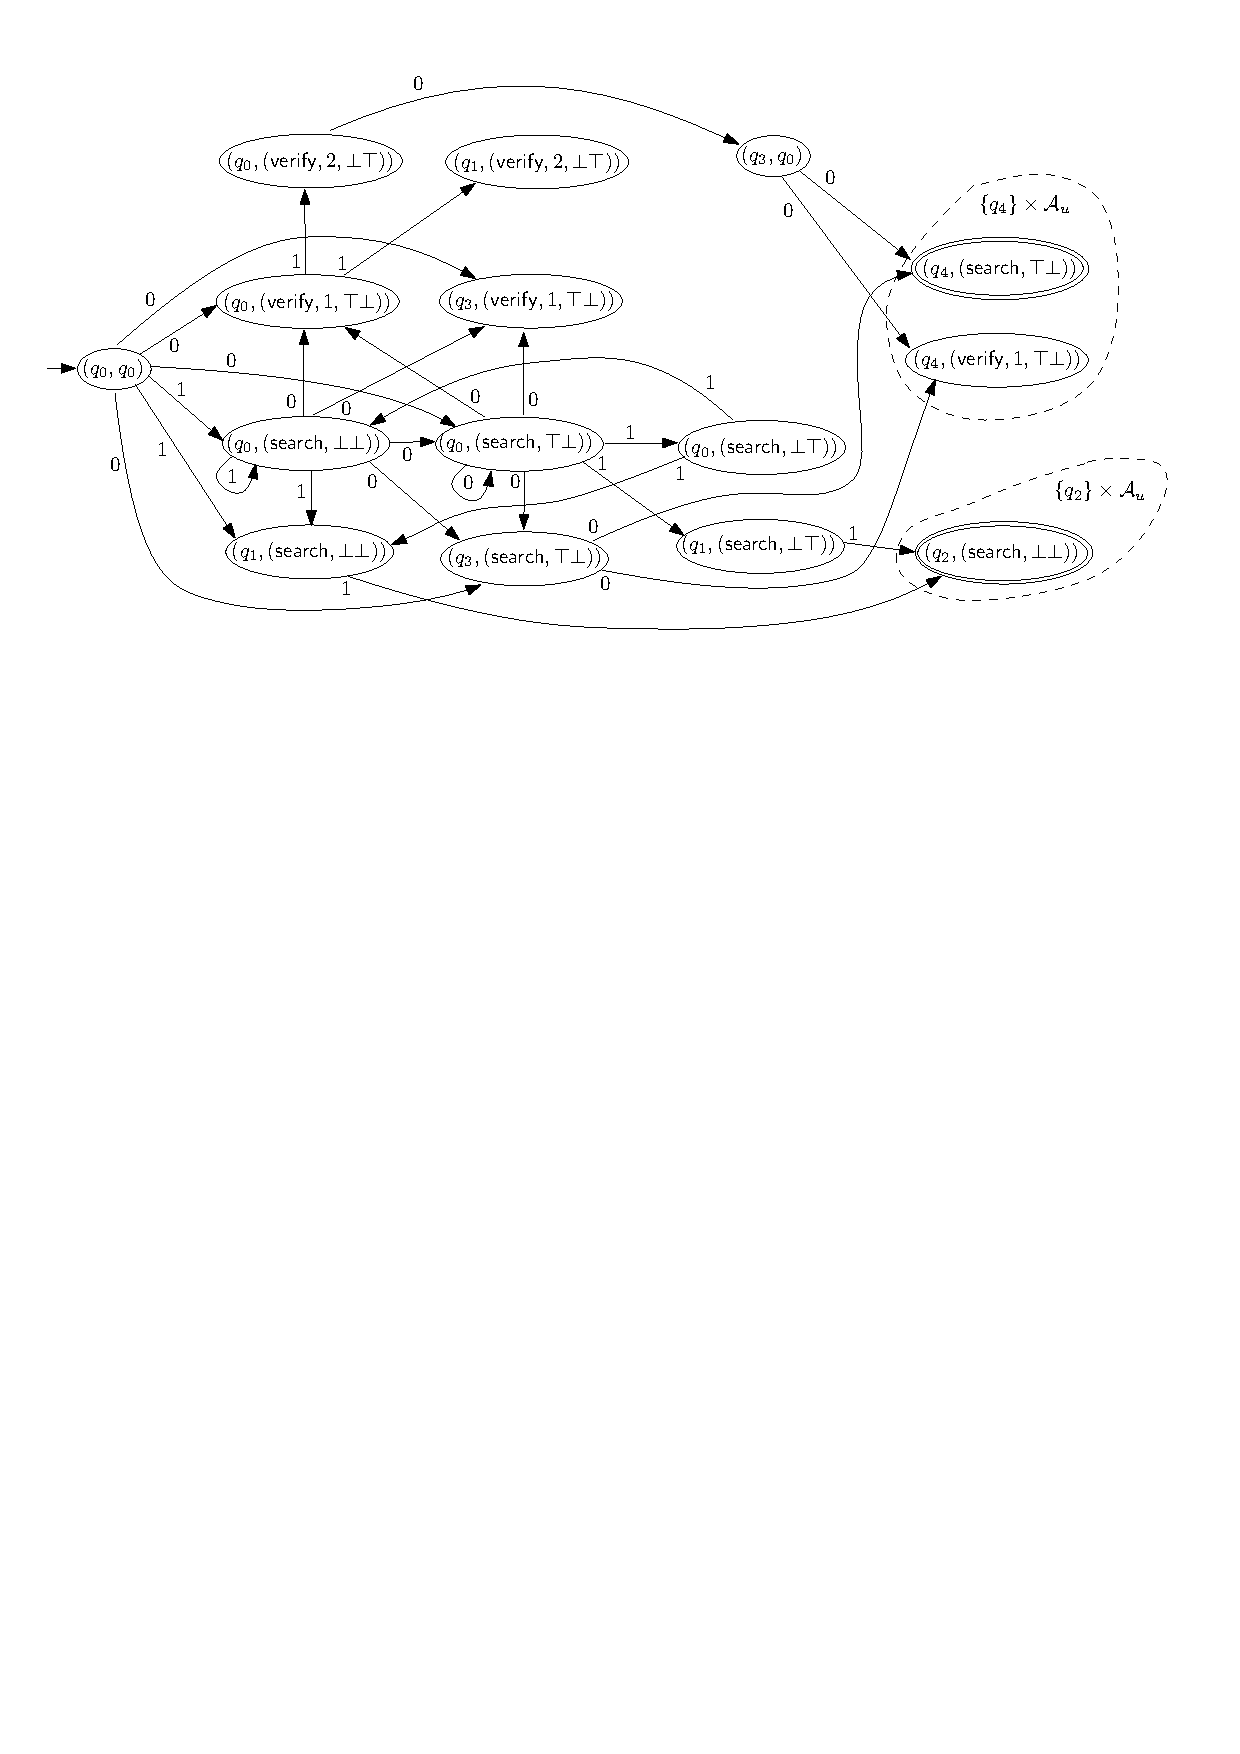
\includegraphics[scale=0.65]{constant-string-example.pdf}
\end{center}
\caption{The NFA $\cA_1 \times \cA_u$ for $u = 010$}\label{fig-cs-exmp}
\end{figure}
%

\def\refsecreplaceallcs{\ref{sec:replaceallcs}}
\section{Complexity analysis in Section~\protect\refsecreplaceallcs}
\label{sec:cs-complexity-full}

We provide a more detailed analysis of the complexity of the algorithm for the constant string case, described in Section~\ref{sec:replaceallcs}.
A summary of this argument already appears in Section~\ref{sec:replaceallcs}.

When constructing $G_{i+1}$ from $G_i$, suppose the two edges from $x$ to $y$ and $z$ respectively are currently removed, let the labels of the two edges be $({\sf l}, u)$ and $({\sf r}, u)$ respectively, then each element $(\cT, \cP)$ of $\cE_i(x)$ may be transformed into an element $(\cT', \cP')$ of $\cE_{i+1}(y)$ such that $|\cT'| = O(|u||\cT|)$, meanwhile, it may also be transformed into an element $(\cT'', \cP'')$ of $\cE_{i+1}(z)$ such that $\cT''$ has the same state space as $\cT$. Thus, for each source variable $x$, $\cE(x)$ contains at most exponentially many elements, and each of them may have a state space of at most exponential size. For instance, for a path from $x'$ to $x$ where the constant strings $u_1,\cdots, u_n$ occur in the labels of edges, an element $(\cT,\cP) \in \cE_0(x')$ may induce an element $(\cT', \cP')$ of $\cE(x)$ such that $|\cT'| \le |\cT| |u_1| \cdots |u_n|$, which is exponential in the worst case. 
%
To solve the nonemptiness problem of the intersection of all these regular constraints, the exponential space is sufficient. Consequently, in this case, we still obtain an EXPSPACE upper bound. 

Let us now consider the special situation that the $\rpleft$-length of $G_C$ is bounded by a constant $c$.
Since $\dmdidx(G_C) \le \lftlen(G_C)$, we know that $\dmdidx(G_C)$ is also bounded by $c$. Therefore, according to Proposition~\ref{prop-di}, there are at most polynomially different paths in $G_C$, we deduce that for each source variable $x$, $\cE(x)$ contains at most polynomially many elements. In addition, since the number of $\rpleft$-edges in each path is bounded by $c$, during the execution of the decision procedure, the number of times when $(\cT, \cP)$ of $\cE_i(x)$ may be transformed into an element $(\cT', \cP')$ of $\cE_{i+1}(y)$ such that $|\cT'| = O(|u||\cT|)$ is bounded by $c$.
Therefore, for each source variable $x$ and each element $(\cT'', \cP'')$ in $\cE(x)$,  $|\cT''|$ is at most polynomial in the size of $C$. We then conclude that for each source variable $x$, $\cE(x)$ corresponds to the intersection of polynomially many regular constraints such that each of them has a state space of polynomial size. Therefore, the nonemptiness of the intersection of all the regular constraints in $\cE(x)$ can be solved in polynomial space. In this situation, we obtain a PSPACE upper bound.


\def\refsecreplaceallre{\ref{sec:replaceallre}}
\section{Complexity analysis in Section~\protect\refsecreplaceallre}
\label{sec:re-complexity-full}

We provide a more detailed analysis of the complexity of the algorithm for the regular-expression case, described in Section~\ref{sec:replaceallre}.
A summary of this argument already appears in Section~\ref{sec:replaceallre}.

In each step of the reduction, suppose the two edges out of $x$ are currently removed, let the two edges be from $x$ to $y$ and $z$ and labeled by $({\sf l}, e)$ and $({\sf r}, e)$ respectively, then each element of $(\cT, \cP)$ of $\cE_i(x)$ may be transformed into an element $(\cT',\cP')$ of $\cE_{i+1}(y)$ such that $|\cT'| = |\cT| \cdot 2^{O(p(|e|))}$, meanwhile, it may also be transformed into an element $(\cT'',\cP'')$ of $\cE_{i+1}(y)$ such that $\cT''$ has the same state space as $\cT$. Thus, after the reduction, for each source variable $x$, $\cE(x)$ may contain exponentially many elements, and each of them may have a state space of exponential size, more precisely, if we start from a vertex $x$ without predecessors, with an element $(\cT,\cP)$ in $\cE_0(x)$, and go to a source variable $y$ through a path where $k$ edges have been traversed and removed, let $e_1,\cdots, e_k$ be the regular expressions occurring in the labels of these edges, then the resulting element in $\cE(y)$ has a state space of size $|\cT| \cdot 2^{O(p(|e_1|))} \cdot 2^{O(p(|e_2|))} \cdot \cdots \cdot 2^{O(p(|e_k|))}$ in the worst case. To solve the nonemptiness problem of the intersection of all these regular constraints, the exponential space is sufficient. Consequently, for the most general case of regular expressions, we still obtain a EXPSPACE upper bound. 

On the other hand, for the situation that the $\rpleft$-length of $G_C$ is at most one, we wan to show that the algorithm runs in polynomial space. Suppose the $\rpleft$-length of $G_C$ is at most one. Then the diamond index of $G_C$ is at most one as well. According to Proposition~\ref{prop-di}, there are only polynomially many paths in $G_C$. Nevertheless, for each source variable $x$, $\cE(x)$ may contain an element $(\cT,\cP)$ such that $|\cT|$ is exponential. Since $|\cP|$ may be exponential, $(\cT,\cP)$ may correspond to the intersection of exponentially many regular constraints. However, we can show that $|\cP|$ is at most polynomial, as a result of the fact that the $\rpleft$-length of $G_C$ is at most one. The arguments proceed as follows: Suppose two edges from $x$ to $y, z$ respectively are removed, and an element $(\cT', \cP')$ of $\cE_{i+1}(y)$ such that $|\cT'|$ is exponential and $|\cP'|$ is polynomial, is generated from an element of $(\cT, \cP)$ of $\cE_i(x)$. Then $y$ must be a source variable in $G_C$. Otherwise, there is an $\rpleft$-edge out of $y$ and the $\rpleft$-length of $G_C$ is at least two, a contradiction. Therefore, $y$ is a source variable in $G_C$, $(\cT', \cP')$  will not be used to generate the regular constraints for the other variables. In other words, $y$ is a source variable in $G_C$, and $(\cT', \cP') \in \cE(y)$ with $|\cP'|$ polynomial. We then conclude that for each source variable $x$, $|\cE(x)|$  is at most polynomial in the size of $C$ and for each element $(\cT, \cP) \in \cE(x)$, $|\cP|$ is polynomial in the size of $C$. Therefore, for each source variable $x$,  $\cE(x)$ corresponds to the intersection of polynomially many regular constraints, where each of them has a state space at most exponential size. To solve the nonemptiness of the intersection of these regular constraints, the polynomial space is sufficient. We obtain a PSPACE upper bound for the situation that the $\rpleft$-length of $G_C$ is at most one.


\def\refsecext{\ref{sec-ext}}
\section{Undecidability Proofs for Section~\protect\refsecext}
\label{sec:ext-undec-proofs}

\subsection{Proof of Theorem~\ref{thm-ext-int}}

\begin{proof}
	The basic idea of the reduction is to simulate the two polynomials $f(x_1,\cdots, x_n)$ and $g(x_1,\cdots, x_n)$, where $x_1,\cdots,x_n$ range over the set of natural numbers, with two $\strline[\concat,\replaceall]$ formulae $C_f, C_g$ over a unary alphabet $\{a\}$, with the output string variables $y_f, y_g$ respectively, and simulate the equality $f(x_1,\cdots, x_n) = g(x_1,\cdots, x_n)$ with the integer constraint $|y_f|=|y_g|$ (which is equivalent to $y_f = y_g$, since $y_f, y_g$ represent strings over the unary alphabet $\{a\}$). 
	
	A polynomial $f(x_1,\cdots, x_n)$ or $g(x_1,\cdots, x_n)$ where $x_1, \cdots, x_n$ range over the set of natural numbers, can be simulated by an $\strline[\concat,\replaceall]$ formula over an unary alphabet $\{a\}$ as follows: The natural numbers are represented by the strings over the alphabet $\{a\}$. A string variable is introduced for each subexpression of $f(x_1,\cdots, x_n)$. The numerical addition operator $+$ is simulated by the string operation $\concat$ 
	%\mat{$\concat$ is not part of $\strline[\replaceall]$, can it be simulated when the string alphabet is unary, or do we need two extra characters?}\zhilin{changed to $\strline[\concat,\replaceall]$.}
	and the multiplication operator $*$ is simulated by $\replaceall$. Since it is easy to figure out how the simulation proceeds, we will only use an example to illustrate it and omit the details here. Let us consider $f(x_1,x_2) = x_1^2 + 2 x_1 x_2 + 5$. By abusing the notation, we also use $x_1,x_2$ as string variables in the simulation. We will introduce a string variable for each subexpression in $f(x_1,x_2)$, namely the variables $y_{x_1^2}, y_{x_1x_2}, y_{2x_1x_2}, y_{x_1^2+2x_1x_2}, y_{f(x_1,x_2)}$. Then $f(x_1,x_2)$ is simulated by the $\strline[\concat,\replaceall]$ formula
	\[
	\begin{array} {l c l }
	C_f & \equiv & y_{x_1^2} = \replaceall(x_1,a, x_1)\ \wedge y_{x_1x_2} = \replaceall(x_1, a, x_2)\ \wedge \\
	& & y_{2x_1x_2} = \replaceall(aa, a, y_{x_1x_2})\ \wedge y_{x_1^2+2x_1x_2} = y_{x_1^2} \concat y_{2x_1x_2}\ \wedge  \\
	& & y_{f(x_1,x_2)}=y_{x_1^2+2x_1x_2} \concat a a a a a\ \wedge x_1 \in a^*\ \wedge x_2 \in a^*.
	\end{array}
	\]
	Then according to Proposition~\ref{prop-concat}, $C_f, C_g$ can be turned into equivalent $\strline[\replaceall]$ formula $C'_f, C'_g$ by introducing fresh letters.
	%\mat{But we may have to give up the unary alphabet?}\zhilin{yes, you are  right, it is fine.}
	
	Since $C'_f$ and $C'_g$ share only source variables $x_1,\cdots, x_n$, we know that $C'_f \wedge C'_g$ is still an $\strline[\replaceall]$ formula.
	From the construction of $C'_f, C'_g$, it is evident that for every pair of polynomials $f(x_1,\cdots, x_n)$ and $g(x_1,\cdots, x_n)$, $f(x_1,\cdots, x_n) = g(x_1,\cdots, x_n)$ has a solution in natural numbers iff $C'_f \wedge C'_g \wedge |y_f| = |y_g|$ is satisfiable. The proof is complete.
	%
	%%%%%%%%%%%%%%%%%%%%%%%%%%%%%%%%%%%%%%%%%%%%%%%%%%%%%%%%%%%
	%%%%%%%%%%%%%%%%%%%%%%%%%%%%%%%%%%%%%%%%%%%%%%%%%%%%%%%%%%%
	\hide{
		We shall reduce from the aforementioned version of the Hilbert tenth problem. For any polynomial with positive integral  $f(x_1, \cdots, x_n)$ where each coefficient is a positive, we can construct a (division-free) arithmetic circuit (AC) is a directed  acyclic graph with nodes labelled with constants from $\mathbb{Z}$, or with some indeterminates $X_1, \cdots, X_m$, or with the operators $+, -, *$. The nodes labelled with constants are called constant nodes, while those labelled with indeterminates are called input nodes. Both constant and input nodes do not have incoming edges. Internal nodes are those labelled with $+,-,*$. Output node is the one which does not have out-going edges. Without loss of generality we assume that each internal node has in-degree 2, and there is only one output node. Each node in the circuit represents a multivariate polynomial $\mathbb{Z}[X_1, \cdots, X_m]$. Vice verse, each polynomial $f\in \mathbb{Z}[X_1, \cdots, X_m]$ can be represented as an AC, and, if the polynomial has only positive (integral) coefficients, the corresponding AC does not contain nodes labelled by $-$ or negative constants.  
		
		We observe that, given an AC, one can construct an SL[$\concat, \replaceall$] formula over the alphabet $\Sigma=\{a\}$ as follows. Each node $n$ of the AC is associated with a string variable $x_n$. As a result, each input node of the AC labelled by $X_i$ (i.e., the indeterminate) corresponds to a  source variable.   
		\begin{itemize}
			\item For each internal node $n$ labelled by $+$, suppose that $n$ has two children nodes $n_l$ and $n_r$, we introduce a string constraint $x_n= x_{n_l}\concat x_{n_l}$.  
			
			\item For each internal node $n$ labelled by $*$, suppose that $n$ has two children nodes $n_l$ and $n_r$, we introduce a string constraint $x_n= \replaceall(x_{n_l}, a, x_{n_l})$.  		
		\end{itemize}
		Furthermore, we introduce, for each node $n$ labelled by a constant $c$, a regular constraint $x_n=a^c$. 
		
		It is straightforward to verify, according to the semantics of SL[$\concat, \replaceall$], that:
		\begin{itemize}
			\item for relational constraint $x_n= x_{n_l}\concat x_{n_l}$, $|x_n|= |x_{n_l}|+|x_{n_l}|$; 
			\item for relational constraint $x_n= \replaceall(x_{n_l}, a, x_{n_l})$,  $|x_n|= |x_{n_l}|\cdot |x_{n_l}|$; and 
			\item for regular $x_n=a^c$, $|x_n|=c$. 
		\end{itemize}
		
		It follows that for each polynomial $f(x_1, \cdots, x_m)$ with positive integral coefficients, we can construct a straight-line string constraint $\varphi_{f}\wedge\psi_g$ over $\Sigma=\{a\}$ with $y_f$ as the output variant and $y_1, \cdots, y_n$ as source variables such that
		$f(c_1, \cdots, c_m)=|y|$ and, for each $1\leq i\leq m$, $|y_i|= c_i$ (i.e., $y_i=a^{c_i}$).  
		
		Consequently, when given two polynomials $f(x_1, \cdots, x_m)$ and $g(x_1, \cdots, x_m)$, we have straight-line string constraints $\varphi_{f}\wedge \varphi_{g}\wedge \psi_{f}\wedge \psi_g$ with two distinguished two variables  $y_f$ and $y_g$ such that  
		\[\exists x_1, \cdots, x_m. f(x_1, \cdots, x_m)=g(x_1, \cdots, x_m)\mbox{ iff } |y_f|=|y_g|\wedge \varphi_{f}\wedge \varphi_{g}\wedge \psi_{f}\wedge \psi_g\mbox{ is satisfiable} \]
		
		Finally, note that any  SL[$\concat, \replaceall$] constraints can be transformed into SL[$\replaceall$] constraints, we obtain a reduction from the Hilbert's 10th problem to the satisfiability problem of  SL[$\replaceall$] with length constraints, which entail that the latter problem is undecidable. The proof is completed. 
	}
	%%%%%%%%%%%%%%%%%%%%%%%%%%%%%%%%%%%%%%%%%%%%%%%%%%%%%%%%%%%
	%%%%%%%%%%%%%%%%%%%%%%%%%%%%%%%%%%%%%%%%%%%%%%%%%%%%%%%%%%%
\end{proof}

\subsection{Undecidability of Depth-1 dependency graph}

A \emph{linear polynomial} (resp.\ quadratic polynomial) is a polynomial with degree at most one (resp.\ with degree at most two) where each coefficient is an integer. %of the form $a_0 + a_1x_1 + \cdots + a_n x_n$ (resp. a polynomial with degree at most two) where each coefficient $a_i\in \mathbb{Z}$  for $0 \leq i \leq n$. A quadratic polynomial

\begin{theorem}[\cite{ID04}]\label{thm-quad-eq}
	%	There exists some (fixed) $k$ such that no algorithm can solve Diophantine systems in the following form
	%	\[y_1F_1=G_1, t_1H_1=I_1, \cdots, t_kF_k = G_k, t_kH_k = I_k,\] 
	%
	%	where $F_i, G_i, H_i, I_i$ for $1\leq i\leq k$ are nonnegative linear polynomials over natural number variables  $s_1, \cdots, s_m$.
	The following problem is undecidable: Determine whether a system of equations of the following form has a solution in natural numbers, 
	\[
	\begin{array} {l l }
	A_i = B_i, & i =1, \cdots, k,\\
	y_iF_i=G_i \wedge y_i H_i = I_i, & i =1, \cdots, m, 
	\end{array}
	\] 
	%
	where $A_i, B_i, F_i, G_i$ are linear polynomials on the variables $x_1,\cdots, x_n$ (Note that each variable $y_i$ occurs in exactly two quadratic equations).
\end{theorem}

We can get a reduction from the problem in Theorem~\ref{thm-quad-eq} to the satisfiability of the extension of $\strline[\replaceall]$ with integer constraints as follows: For each monomial $y_i x_j$ in the quadratic polynomials, we use an $\strline[\replaceall]$ formula $z_{y_i x_j} = \replaceall(y_i, a, x_j)$ to simulate $y_i x_j$, where $z_{y_i x_j}$ are freshly introduced string variables. Since each equation $y_iF_i=G_i$ or $y_i H_i = I_i$ can be seen as a linear combination of the terms $y_i x_j$ and $x_j$ for $i \in [m]$ and $j \in [n]$, we can replace each variable $x_j$ with $|x_j|$, and each term $y_ix_j$ with $|z_{y_i x_j}|$,  thus transform them into the (linear) integer constraints $F'_i = G'_i$ or $H'_i = I'_i$. Similarly, after replacing each variable $x_j$ with $|x_j|$, we transform each equation $A_i= B_i$ into an integer constraint $A'_i = B'_i$. Therefore, we get a formula 
$$
\begin{array}{l c l }
\bigwedge \limits_{i \in [m], j \in [n]} z_{y_i x_j} = \replaceall(y_i, a, x_j) \wedge \bigwedge \limits_{i \in [m]} y_i \in a^*\ \wedge  \bigwedge \limits_{j \in [n]} x_j \in a^* \  \wedge\\
\hspace{2cm} \bigwedge \limits_{i \in [k]} A'_i = B'_i \wedge \bigwedge \limits_{i \in [m]} (F'_i = G'_i \wedge H'_i = I'_i),
\end{array}
$$
where the dependency graph of the $\strline[\replaceall]$ subformula is of depth at most one.

%%%%%%%%%%%%%%%%%%%%%%%%%%%%%%%%%%%%%%%%%%%%%%%%%
%%%%%%%%%%%%%%%%%%%%%%%%%%%%%%%%%%%%%%%%%%%%%%%%%
\hide{
	From this class of quadratic Diophantine equations, we can introduce string variables $x_1, \cdots, x_k$ and $y_1, \cdots, y_m$, together with relational string constraints 
	\[z_{i,j}=\replaceall(x_i, a, y_j)\]
	for $1\leq i\leq k$ and $1\leq j\leq m$. Note that, for each $i$,  $t_i F_i=G_i$ can be written as
	\begin{equation} \label{eq:dio}
	t_i\cdot \left(a_0+\sum_{j=1}^s a_j s_j\right) =  b_0+\sum_{j=1}^s b_j s_j
	\end{equation}
	where $a$'s and $b$'s are all natural numbers. Moreover, \eqref{eq:dio} holds iff 
	\[a_0\cdot |y_i|+ \sum_{j=1}^s a_j |z_{i,j}| =  b_0+ \sum_{j=1}^s b_j |x_j| \] 
	which is an integer constraint defined in Definition~\ref{def:intconst}. This entails that
}
%%%%%%%%%%%%%%%%%%%%%%%%%%%%%%%%%%%%%%%%%%%%%%%%%
%%%%%%%%%%%%%%%%%%%%%%%%%%%%%%%%%%%%%%%%%%%%%%%%%

\subsection{Undecidability of the character constraints}

\begin{proposition}\label{prop-ext-char}
	For the extension of $\strline[\replaceall]$ with character constraints, the satisfiability problem is undecidable. 
\end{proposition}

The arguments for Proposition~\ref{prop-ext-char} proceed as follows. Recall that in the proof of Theorem~\ref{thm-ext-int}, we get a formula $C_f \wedge C_g \wedge |y_f| = |y_g|$ such that $f(x_1,\cdots, x_n) = g(x_1,\cdots, x_n)$ has a solution in natural numbers iff $C_f \wedge C_g \wedge |y_f| = |y_g|$ is satisfiable. Let $\$ \neq a$. Suppose  $z_f = y_f \concat \$$, and $z_g = y_g \concat \$$. Then $|y_f| = |y_g|$ can be captured by $z_f[\mathfrak{n}] = \$[1] \wedge  z_g[\mathfrak{n}] = \$[1]$, where $\mathfrak{n}$ is a variable of type $\intnum$. More precisely, 
%
we have 
\begin{quote}
	\centering
	$C_f \wedge C_g \wedge |y_f|= |y_g|$ is satisfiable \\
	%
	iff \\
	%
	$C_f \wedge C_g \wedge z_f = y_f \concat \$ \wedge z_g = y_g \concat \$ \wedge z_f[\mathfrak{n}] = \$[1] \wedge  z_g[\mathfrak{n}] = \$[1]$ is satisfiable. 
\end{quote}
Therefore, we get a reduction from Hilbert's tenth problem to the satisfiability problem for the extension of $\strline[\replaceall]$ with character constraints. 

%For any two string variables $x,y$ on the unary alphabet $\{a\}$, let $x' = x \concat \$$ and $y' = y \concat \$$, then $|x| = |y|$ iff .
%
% $|x|=|y|$ iff $\exists n. x[n]=y[n]=\$$. 
%
%
%\begin{lemma}
%	For any two strings $x,y\in a^*\$$, $|x|=|y|$ iff $\exists n. x[n]=y[n]=\$$. 
%\end{lemma}
%
%As SL[$\replaceall$] with length constraints is undecidable, we conclude that 
%
%
%
%\tl{I am not satisfied with this as the quantifier is used}

\subsection{Undecidability of the $\indexof$ constraints}

\begin{proposition}\label{prop-indexof}
	For the extension of $\strline[\replaceall]$ with the $\indexof$ constraints, the satisfiability problem is undecidable. 
\end{proposition}

Proposition~\ref{prop-ext-char} follows from the following observation and Theorem~\ref{thm-ext-int}: For any two string variables $x,y$ over a unary alphabet, 
$1= \indexof(x,y)$ iff $x$ is a prefix of $y$. Therefore, $|x| = |y|$ iff $1=  \indexof(x,y) \wedge 1= \indexof(y,x)$. This implies that in the proof of Theorem~\ref{thm-ext-int}, we can replace $|y_f| = |y_g|$ with $1=\indexof(y_f, y_g) \wedge 1 = \indexof(y_g, y_f)$ and get a reduction from Hilbert's tenth problem to the satisfiability problem for the extension of $\strline[\replaceall]$ with the $\indexof$ constraints.
Note that $=$ can be simulated as a conjunction of $\leq$ and $\geq$.


%We have the following observation: 
%\begin{lemma}
%	For any two strings $x,y$ over $\{a\}$, $x=y$ iff $1=\indexof(x,y)=\indexof(y,x)$.  
%\end{lemma}
%
%It follows that 

%\subsection*{Further undecidability results}


\def\refsecreplaceallre{\ref{sec:replaceallre}}
\section{Examples in Section~\protect\refsecreplaceallre}

\begin{example}\label{exmp-pa-re}
	Let $e_0 = 0^*0 1(1^* + 0^*)$. Then $\cA_{0}$ and $\cA_{e_0}$ are illustrated in Figure~\ref{fig-pa-re}, where ${\sf sleft}$ and ${\sf slong}$ are the abbreviations of $\searchleft$ and $\searchlong$ respectively. Let us use the state $(\{q_{0,1}\}\{q_{0,0}\}, {\sf sleft}, \emptyset)$ to illustrate the construction. Since $\big(\delta_0(\{q_{0,1}\}, 0) \cup \delta_0(\{q_{0,0}\}, 0)\big) \cap F_0 = \{q_{0,1}\} \cap F_0 = \emptyset$, $\delta_0(\emptyset, 0) \cap F_0 = \emptyset$, and $\red(\delta_0(\{q_{0,1}\}, 0) \delta_0(\{q_{0,0}\}, 0))=\{q_{0,1}\}$, we deduce that the transition $((\{q_{0,1}\}\{q_{0,0}\}, {\sf sleft}, \emptyset), 0, (\{q_{0,1}\} \{q_{0,0}\}, {\sf sleft}, \emptyset)) \in \delta_{e_0}$. On the other hand, it is impossible to go from the state $(\{q_{0,1}\}\{q_{0,0}\}, {\sf sleft}, \emptyset)$ to the ``$\searchlong$'' mode. This is due to the fact that $\delta_0(\{q_{0,0}\}, 0)=\{q_{0,1}\} \subseteq \delta_0(\{q_{0,1}\},0)=\{q_{0,1}\}$. In addition, there are no $1$-transitions out of $(\{q_{0,1}\}\{q_{0,0}\}, {\sf sleft}, \emptyset)$. This is due to the fact that $\delta_0(\{q_{0,1}\}, 1) \cap F_0 = \{q_{0,2}, q_{0,3}\} \cap F_0 \neq \emptyset$.
	%
	\begin{figure}[htbp]
		\begin{center}
			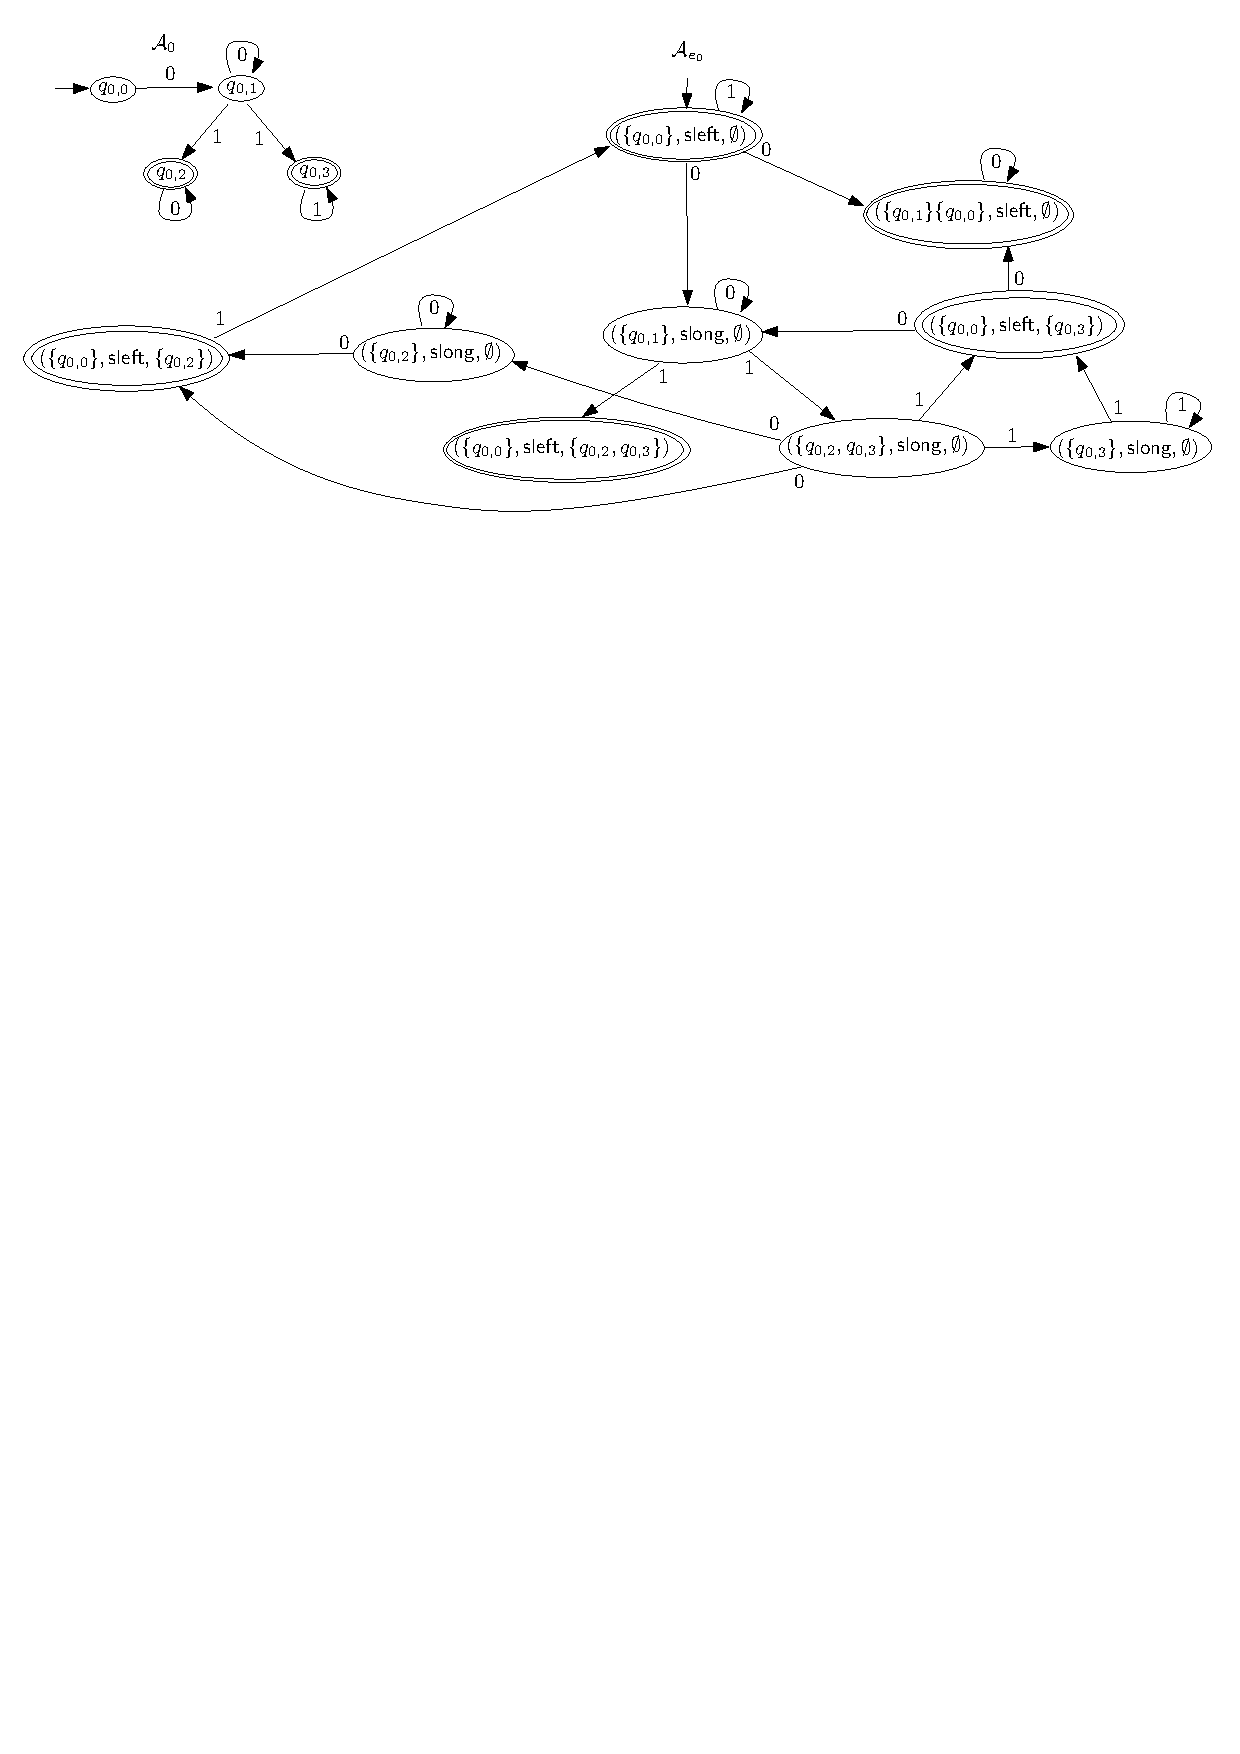
\includegraphics[scale=0.7]{regular-expression-example.pdf}
		\end{center}
		\caption{The NFA $\cA_0$ and $\cA_{e_0}$ for $e_0 = 0^*0 1(1^* + 0^*)$}\label{fig-pa-re}
	\end{figure} 
\end{example}

\begin{example}
	Let $C \equiv x = \replaceall(y, e_0, z) \wedge x \in e_1 \wedge y \in e_2 \wedge z \in e_3$, where $e_1,e_2,e_3$ are as in Example~\ref{exmp-sl} (cf. Figure~\ref{fig-sl-exmp}) and $e_0$ is as in Example~\ref{exmp-pa-re} (cf. Figure~\ref{fig-pa-re}). Suppose $T_z = \{(q_0, q_0), (q_1, q_2)\}$. Then the NFA $\cB_{\cA_1, e_0, T_z}$ is as illustrated in Figure~\ref{fig-re-exmp}, where the thick edges denote the added transitions. Let us use the state $(q_1, (\{q_{0,0}\}, \searchleft, \emptyset))$ to exemplify the construction. The transition $((q_1, (\{q_{0,0}\}, \searchleft, \emptyset)), 1, (q_2, (\{q_{0,0}\}, \searchleft, \emptyset)))$ is  in $\cA_1 \times \cA_{e_0}$. Since $\delta_0(q_{0,0}, 1) \cap F_0 = \emptyset$, this transition is not removed and is thus in $\cB_{\cA_1, e_0, T_z}$. On the other hand, since there are no $0$-transitions out of $q_1$ in $\cA_1$, there are no $0$-transitions from $(q_1, (\{q_{0,0}\}, \searchleft, \emptyset))$ to some state from $Q_{\searchleft}$ in $\cB_{\cA_1, e_0, T_z}$. 
	Moreover, because $((\{q_{0,0}\}, \searchleft, \emptyset), 0, (\{q_{0,1}\}, \searchlong, \emptyset)) \in \delta_{e_0}$ and $(q_1, q_2) \in T_z$, the transition $((q_1, (\{q_{0,0}\}, \searchleft, \emptyset)), 0, (q_1, (\{q_{0,1}\}, \searchlong, \emptyset)))$ is added. 
	One may also note that there are no 0-transitions from $(q_2, (\{q_{0,0}\}, \searchleft, \emptyset))$ to the state $(q_2, (\{q_{0,1}\}, \searchlong, \emptyset))$, because there are no pairs $(q2,-) \in T_z$.
	It is not hard to see that $010101 \in \Ll(\cA_2) \cap \Ll(\cB_{\cA_1, e_0, T_z})$. In addition, $10 \in \Ll(\cA_3) \cap \Ll(\cA_1(q_0,q_0)) \cap \Ll(\cA_1(q_1,q_2))$. Let $y$ be $010101$ and $z$ be $10$. Then $x$ takes the value $\replaceall(010101, e_0, 10)=10 \cdot \replaceall(101, e_0, 10)=10110$, which is accepted by $\cA_1$. Therefore, $C$ is satisfiable.
	\begin{figure}[htbp]
		\begin{center}
			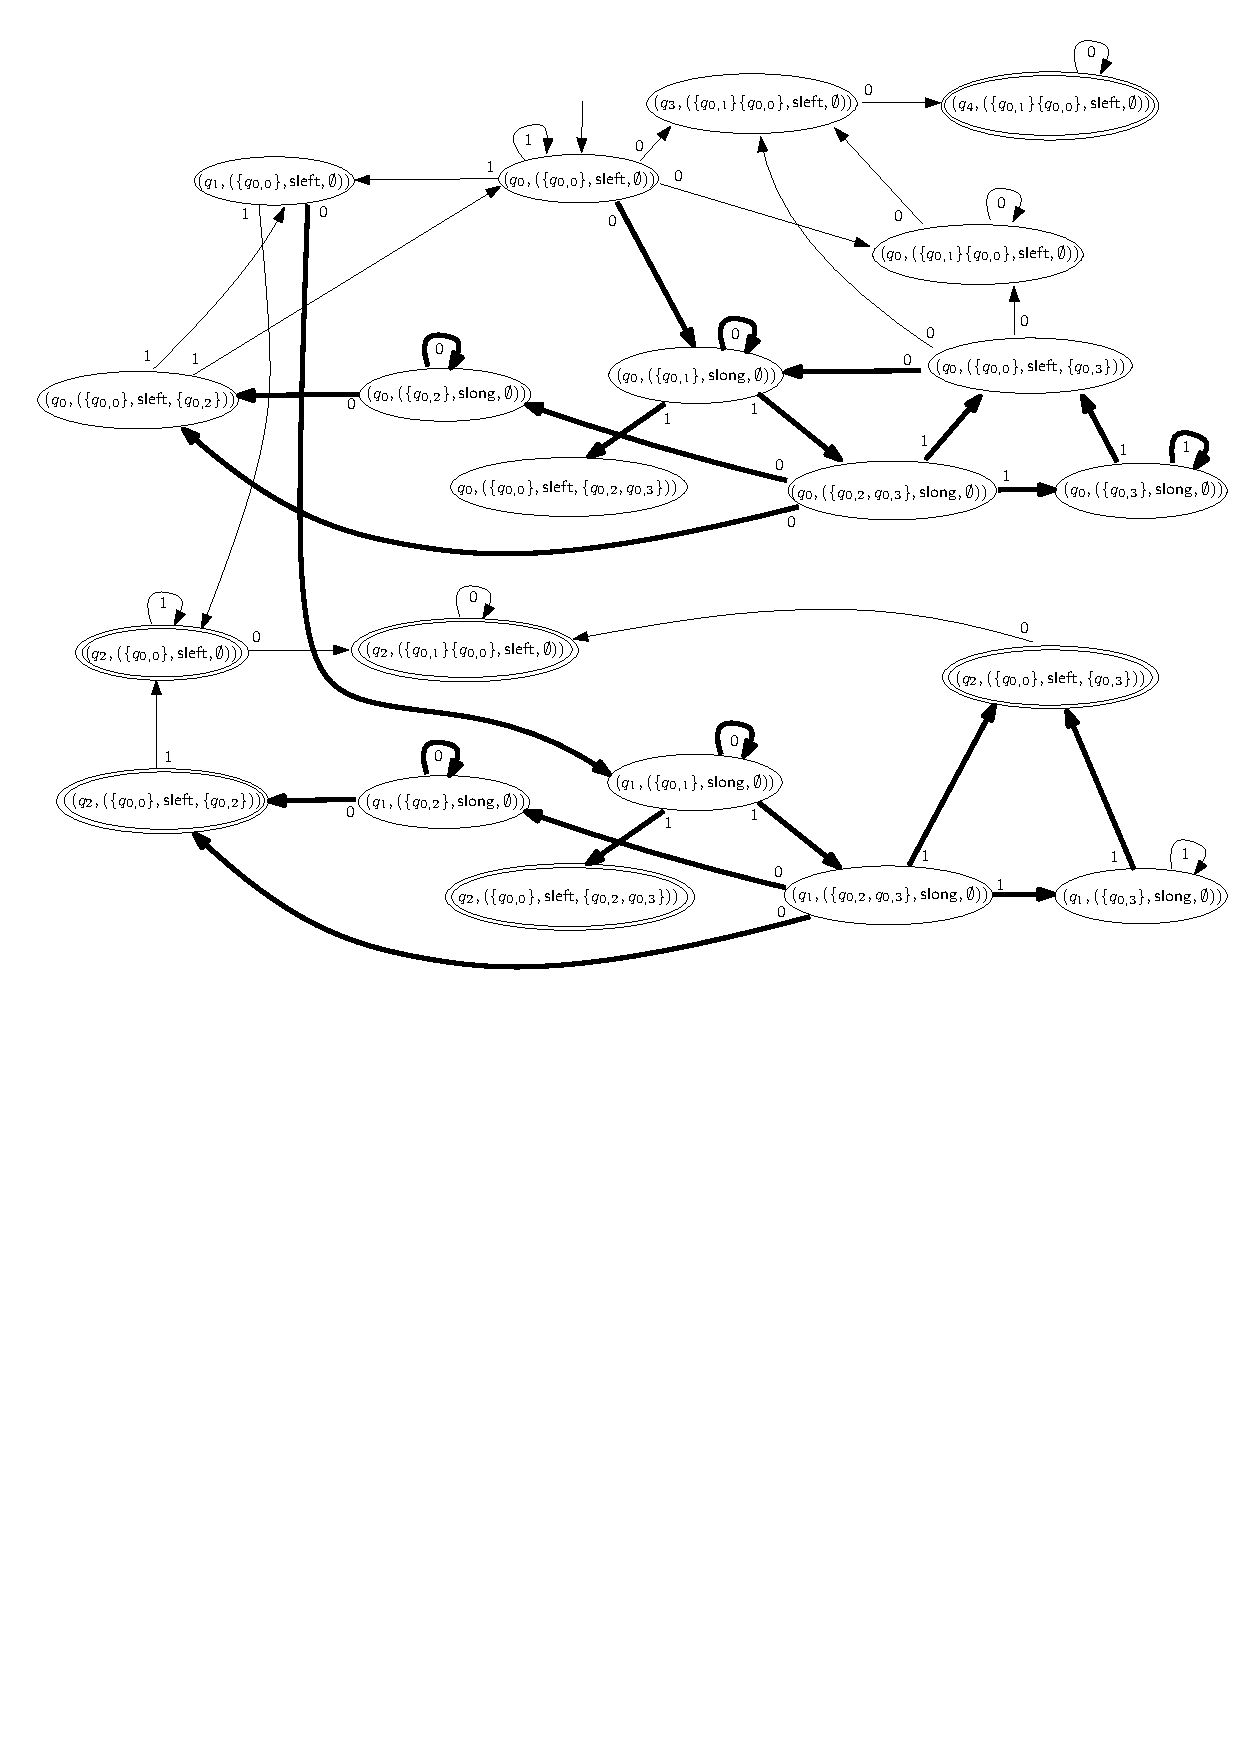
\includegraphics[scale=0.68]{regular-expression-example-2.pdf}
		\end{center}
		\caption{The NFA $\cB_{\cA_1, e_0, T_z}$}\label{fig-re-exmp}
	\end{figure} 
\end{example}



\end{document}
